\documentclass[14pt]{extarticle}

\usepackage[table]{xcolor} % colored lines for tables
\usepackage[normalem]{ulem} % strike through text
\usepackage{amsmath,mathtools,amsfonts,amsthm,amssymb,hyperref}
\usepackage{parskip,geometry,latexsym,bookmark,mathtools,float,cancel}
\usepackage{tcolorbox,bm}

\newtheorem{defn}{Definition}
\newtheorem{thm}{Theorem}
\newtheorem{claim}{Claim}
\newtheorem{lemma}{Lemma}

\newcommand{\dps}{\displaystyle}
\newcommand{\es}{\varnothing}
\newcommand{\eps}{\varepsilon}
\newcommand{\fbl}{\underline{\hspace{1cm}}\,\,}
\newcommand{\R}{\mathbb{R}}
\newcommand{\Q}{\mathbb{Q}}
\newcommand{\Z}{\mathbb{Z}}
\newcommand{\from}{\leftarrow}
\newcommand{\true}{{\bf t}}
\newcommand{\false}{{\bf c}}
\newcommand{\bic}{\leftrightarrow}
\newcommand{\da}{\downarrow}
\newcommand{\ua}{\uparrow}
\newcommand{\fa}{\forall}
\newcommand{\te}{\exists}
\newcommand{\cy}{\color{cyan}}

\newcommand{\colsq}[1]{{\color{#1} $\blacksquare$}}

\newcommand{\base}[1]{{\cy #1}} % for log bases
\newcommand{\floor}[1]{{\left\lfloor#1\right\rfloor}}
\newcommand{\ceil}[1]{{\left\lceil#1\right\rceil}}
\newcommand\Ccancel[2][black]{\renewcommand\CancelColor{\color{#1}}\cancel{#2}}
\newcommand\Cbcancel[2][black]{\renewcommand\CancelColor{\color{#1}}\bcancel{#2}}

%\renewcommand{\arraystretch}{1.2}
\setlength{\extrarowheight}{10pt}

\hypersetup{colorlinks,allcolors=blue,linktoc=all}
\geometry{a4paper}
\geometry{margin=0.42in}

\title{Chapter 11 Solutions, Susanna Epp Discrete Math 5th Edition}

\author{https://github.com/spamegg1}

\begin{document}
\maketitle
\tableofcontents


\section{Exercise Set 11.1}

\subsection{Exercise 1}
\begin{figure}[ht!]
\centering
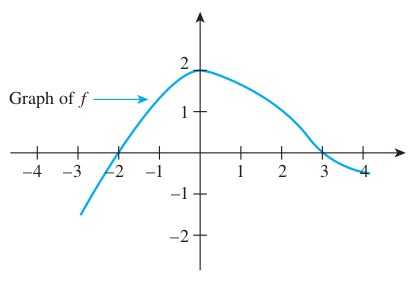
\includegraphics[scale=0.5]{../images/11.1.1.png}
\end{figure}

The graph of a function \(f\) is shown above.

\subsubsection{(a)}
Is \(f(0)\) positive or negative?
\begin{proof}
positive
\end{proof}

\subsubsection{(b)}
For what values of \(x\) does \(f(x) = 0\)?
\begin{proof}
\(f(x) = 0\) when \(x = -2\) and \(x = 3\) (approximately)
\end{proof}

\subsubsection{(c)}
Find approximate values for \(x_1\) and \(x_2\) so that \(f(x_1) = f(x_2) = 1\) but \(x_1 \neq x_2\).
\begin{proof}
\(x_1 = -1\) and \(x_2 = 2\) (approximately)
\end{proof}

\subsubsection{(d)}
Find an approximate value for \(x\) such that \(f(x) = 1.5\).
\begin{proof}
\(x = 1\) or \(x = -1/2\) (approximately)
\end{proof}

\subsubsection{(e)}
As \(x\) increases from \(-3\) to \(-1\), do the values of \(f\) increase or decrease?

\begin{proof}
increase
\end{proof}

\subsubsection{(f)}
As \(x\) increases from 0 to 4, do the values of \(f\) increase or decrease?

\begin{proof}
decrease
\end{proof}

\subsection{Exercise 2}
\begin{figure}[ht!]
\centering
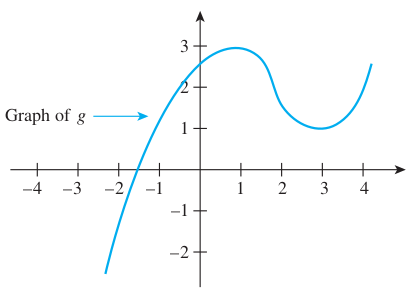
\includegraphics[scale=0.5]{../images/11.1.2.png}
\end{figure}

The graph of a function \(g\) is shown above.

\subsubsection{(a)}
Is \(g(0)\) positive or negative?
\begin{proof}
positive
\end{proof}

\subsubsection{(b)}
Find an approximate value of \(x\) so that \(g(x) = 0\).
\begin{proof}
\(-1.5\) (approximately)
\end{proof}

\subsubsection{(c)}
Find approximate values for \(x_1\) and \(x_2\) so that \(g(x_1) = g(x_2) = 1\) but \(x_1 \neq x_2\).
\begin{proof}
\(x_1 = -1, x_2 = 3\) (approximately)
\end{proof}

\subsubsection{(d)}
Find an approximate value for \(x\) such that \(g(x) = -2\).
\begin{proof}
\(x = -2.2\) (approximately)
\end{proof}

\subsubsection{(e)}
As \(x\) increases from \(-2\) to \(1\), do the values of \(g\) increase or decrease?

\begin{proof}
increase
\end{proof}

\subsubsection{(f)}
As \(x\) increases from 1 to 3, do the values of \(g\) increase or decrease?

\begin{proof}
decrease
\end{proof}

\subsection{Exercise 3}
Sketch the graphs of the power functions \(p_{1/3}\) and \(p_{1/4}\) on the same set of axes. When \(0 < x < 1\), which 
is greater: \(x^{1/3}\) or \(x^{1/4}\)? When \(x > 1\), which is greater: \(x^{1/3}\) or \(x^{1/4}\)?

\begin{proof}
\begin{figure}[ht!]
\centering
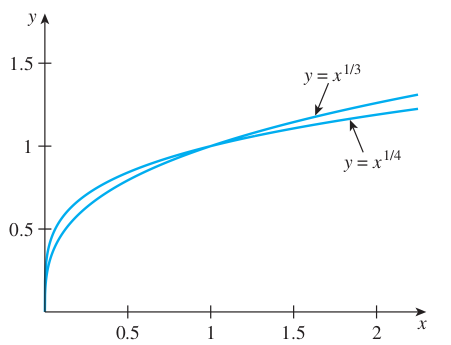
\includegraphics[scale=0.5]{../images/11.1.3.png}
\end{figure}
When \(0 < x < 1\), \(x^{1/3} < x^{1/4}\). When \(1 < x\), \(x^{1/4} < x^{1/3}\).
\end{proof}

\subsection{Exercise 4}
Sketch the graphs of the power functions \(p_3\) and \(p_4\) on the same set of axes. When \(0 < x < 1\), which is greater: 
\(x^3\) or \(x^4\)? When \(x > 1\), which is greater: \(x^3\) or \(x^4\)?

\begin{proof}
\begin{figure}[ht!]
\centering
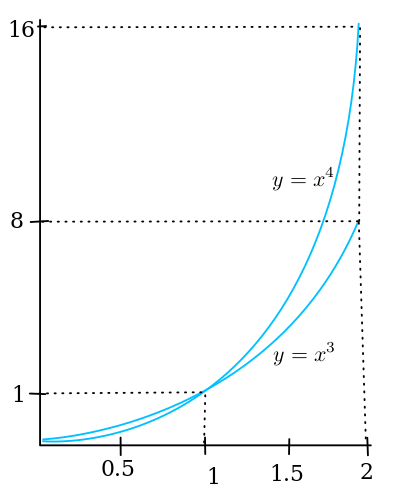
\includegraphics[scale=0.4]{../images/11.1.4.png}
\end{figure}
When \(0 < x < 1\), \(x^4 < x^3\). When \(1 < x\), \(x^3 < x^4\).
\end{proof}

\subsection{Exercise 5}
Sketch the graphs of \(y = 2\floor{x}\); and \(y = \floor{2x}\) for each real number \(x\). What can you conclude from 
these graphs?

\begin{proof}
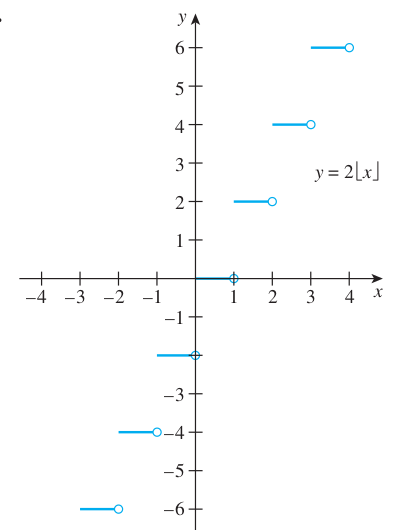
\includegraphics[scale=0.5]{../images/11.1.5.a.png}
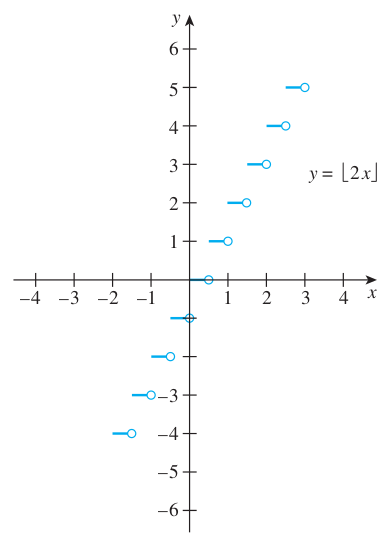
\includegraphics[scale=0.5]{../images/11.1.5.b.png}

The graphs show that \(2\floor{x} \neq \floor{2x}\) for many values of \(x\).
\end{proof}

{\bf \cy Sketch a graph for each of the functions defined in \(6-9\) below.}

\subsection{Exercise 6}
\(g(x) = \ceil{x}\) for each real number \(x\) (Recall that the ceiling of \(x\), \(\ceil{x}\), is the least integer that 
is greater than or equal to \(x\). That is, \(\ceil{x} =\) the unique integer \(n\) such that \(n-1 < x \leq n\).

\begin{proof}
\begin{figure}[ht!]
\centering
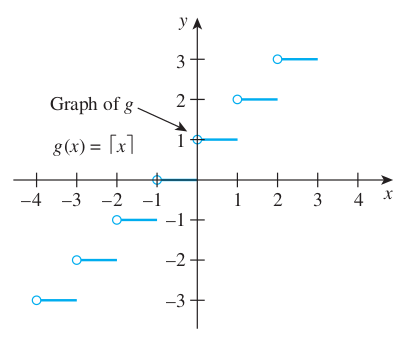
\includegraphics[scale=0.5]{../images/11.1.6.png}
\end{figure}
\end{proof}

\subsection{Exercise 7}
\(h(x) = \ceil{x} - \floor{x}\) for each real number \(x\)

\begin{proof}
\begin{figure}[ht!]
\centering
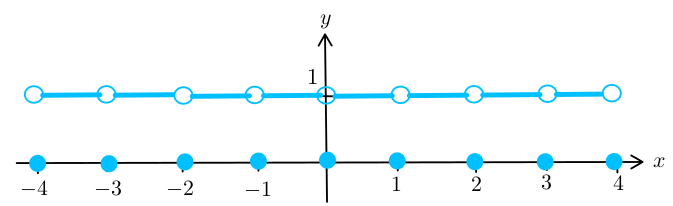
\includegraphics[scale=0.5]{../images/11.1.7.png}
\end{figure}
\end{proof}

\subsection{Exercise 8}
\(F(x) = \floor{x^{1/2}}\) for each real number \(x\)

\begin{proof}
\begin{figure}[ht!]
\centering
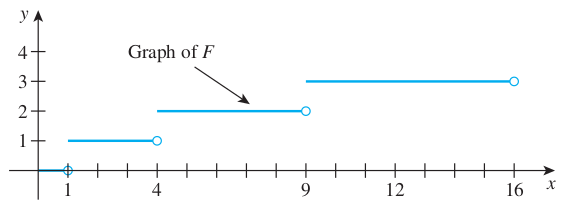
\includegraphics[scale=0.5]{../images/11.1.8.png}
\end{figure}
\end{proof}

\subsection{Exercise 9}
\(G(x) = x - \floor{x}\) for each real number \(x\)

\begin{proof}
\begin{figure}[ht!]
\centering
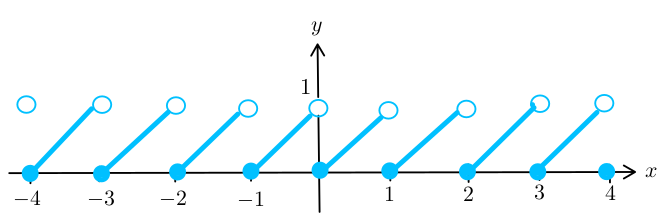
\includegraphics[scale=0.5]{../images/11.1.9.png}
\end{figure}
\end{proof}

{\bf \cy In each of \(10-13\) a function is defined on a set of integers. Sketch a graph for each function.}

\subsection{Exercise 10}
\(f(n) = |n|\) for each integer \(n\)

\begin{proof}
\begin{figure}[ht!]
\centering
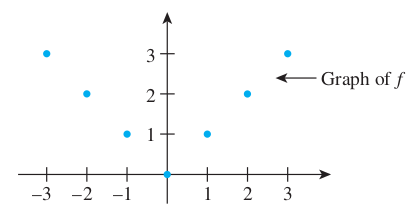
\includegraphics[scale=0.5]{../images/11.1.10.png}
\end{figure}
\end{proof}

\subsection{Exercise 11}
\(g(n) = (n/2) + 1\) for each integer \(n\)

\begin{proof}
\begin{figure}[ht!]
\centering
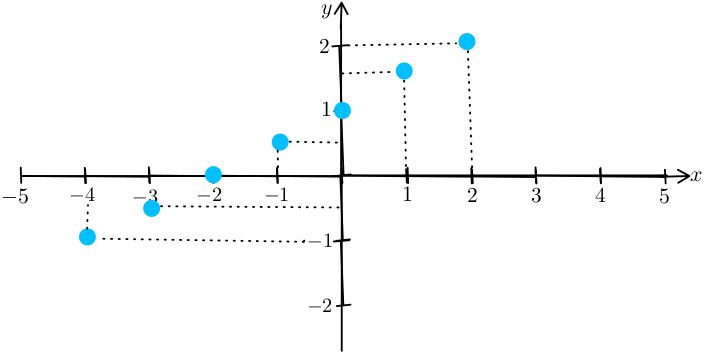
\includegraphics[scale=0.5]{../images/11.1.11.png}
\end{figure}
\end{proof}

\subsection{Exercise 12}
\(h(n) = \floor{n/2}\) for each integer \(n \geq 0\)

\begin{proof}
\begin{figure}[ht!]
\centering
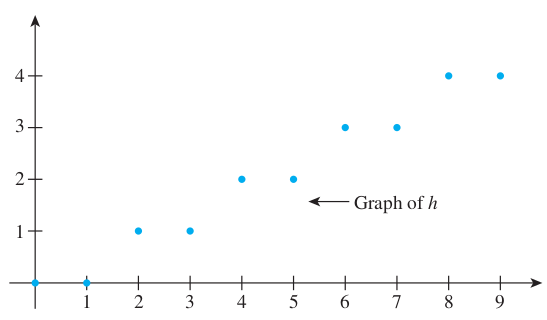
\includegraphics[scale=0.5]{../images/11.1.12.png}
\end{figure}
\end{proof}

\subsection{Exercise 13}
\(k(n) = \floor{n^{1/2}}\) for each integer \(n \geq 0\)

\begin{proof}
\begin{figure}[ht!]
\centering
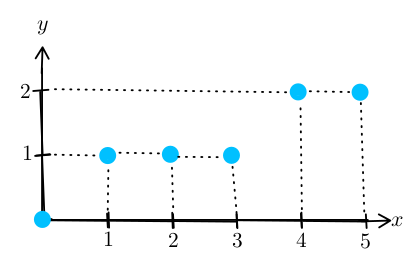
\includegraphics[scale=0.5]{../images/11.1.13.png}
\end{figure}
\end{proof}

\subsection{Exercise 14}
\begin{figure}[ht!]
\centering
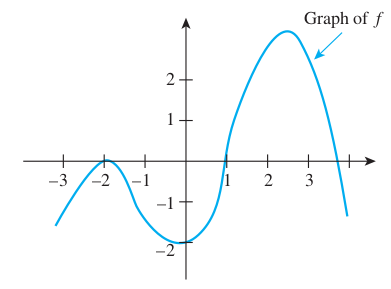
\includegraphics[scale=0.5]{../images/11.1.14.png}
\end{figure}

The graph of a function \(f\) is shown below. Find the intervals on which \(f\) is increasing and the intervals on 
which \(f\) is decreasing.

\begin{proof}
\(f\) is increasing on the intervals \(\{x \in \R \,|\, -3 < x < -2\}\) and \(\{x \in \R \,|\, 0 < x < 2.5\}\), and \(f\) is 
decreasing on \(\{x \in \R \,|\, -2 < x < 0\}\) and \(\{x \in \R \,|\, 2.5 < x < 4\}\) (approximately).
\end{proof}

\subsection{Exercise 15}
Show that the function \(f: \R \to \R\) defined by the formula \(f(x) = 2x - 3\) is increasing on the set of real numbers.

\begin{proof}
Suppose that \(x_1\) and \(x_2\) are particular but arbitrarily chosen real numbers such that \(x_1 < x_2\). 
{\it [We must show that \(f(x_1) < f(x_2)\).]} Since \(x_1 < x_2\) then \(2x_1 < 2x_2\) and \(2x_1 - 3 < 2x_2 - 3\) by 
basic properties of inequalities. Thus, by definition of \(f\), \(f(x_1) < f(x_2)\) {\it [as was to be shown]}. 
Hence \(f\) is increasing on the set of all real numbers.
\end{proof}

\subsection{Exercise 16}
Show that the function \(g: \R \to \R\) defined by the formula \(g(x) = -(x/3) + 1\) is decreasing on the set of real 
numbers.

\begin{proof}

\end{proof}

\subsection{Exercise 17}
Let \(h\) be the function from \(\R\) to \(\R\) defined by the formula \(h(x) = x^2\) for each real number \(x\).

\subsubsection{(a)}
Show that \(h\) is decreasing on the set of real numbers less than zero.

\begin{proof}
Suppose that \(x_1\) and \(x_2\) are particular but arbitrarily chosen real numbers such that \(x_1 < x_2 < 0\). 
{\it [We must show that \(h(x_1) > h(x_2)\).]} 

Since \(x_1 < x_2 < 0\) then \(0 < -x_2 < -x_1\) and multiplying by \(-x_1\) (which is a positive number) we get 
\((-x_1)(-x_2) < (-x_1)(-x_1) = x_1^2\) by basic properties of inequalities. 

Similarly, since \(x_1 < x_2 < 0\) then \(0 < -x_2 < -x_1\) and multiplying by \(-x_2\) (which is a positive number) we 
get \((-x_2)(-x_2) = x_2^2 < (-x_1)(-x_2)\) by basic properties of inequalities. 

By combining the two results we get \(x_2^2 < (-x_1)(-x_2) < x_1^2\) so \(x_2^2 < x_1^2\).

Thus, by definition of \(h\), \(h(x_1) > h(x_2)\) {\it [as was to be shown]}. Hence \(h\) is increasing on the set of all 
real numbers.
\end{proof}

\subsubsection{(b)}
Show that \(h\) is increasing on the set of real numbers greater than zero.

\begin{proof}
Suppose that \(x_1\) and \(x_2\) are particular but arbitrarily chosen real numbers such that \(0 < x_1 < x_2\). 
{\it [We must show that \(h(x_1) < h(x_2)\).]} 

Since \(0 < x_1 < x_2\) then multiplying by \(x_1\) (which is a positive number) we get \(x_1x_1 = x_1^2 < x_1x_2\) by basic 
properties of inequalities. 

Similarly, since \(0 < x_1 < x_2\) then multiplying by \(x_2\) (which is a positive number) we get \(x_1x_2 < x_2x_2 = 
x_2^2\) by basic properties of inequalities. 

By combining the two results we get \(x_1^2 < x_1x_2 < x_2^2\) so \(x_1^2 < x_2^2\).

Thus, by definition of \(h\), \(h(x_1) < h(x_2)\) {\it [as was to be shown]}. Hence \(h\) is increasing on the set of all 
real numbers.
\end{proof}

\subsection{Exercise 18}
Let \(k: \R \to \R\) be the function defined by the formula \(k(x) = (x - 1)/x\) for each real number \(x \neq 0\).

\subsubsection{(a)}
Show that \(k\) is increasing for every real number \(x > 0\).

\begin{proof}
Suppose that \(x_1\) and \(x_2\) are positive real numbers and \(x_1 < x_2\). {\it [We must show that \(k(x_1) < k(x_2)\).]} 

\begin{center}
\begin{tabular}{cll}
& \(x_1 < x_2\) & {\cy by assumption} \\
\(\implies\) & \(-x_2 < -x_1\) & {\cy by multiplying by \(-1\)} \\
\(\implies\) & \(x_1x_2 - x_2 < x_1x_2 - x_1\) & {\cy by adding \(x_1x_2\) to both sides} \\
\(\implies\) & \(x_2(x_1 - 1) < x_1(x_2 - 1)\) & {\cy by factoring both sides} \\
\(\implies\) & \(\dps \frac{x_1 - 1}{x_1} < \frac{x_2 - 1}{x_2}\) & {\cy by dividing both sides by \(x_1x_2 > 0\)} \\
\(\implies\) & \(k(x_1) < k(x_2)\) & {\cy by definition of \(k\)}
\end{tabular}
\end{center}

\end{proof}

\subsubsection{(b)}
Is \(k\) increasing or decreasing for \(x < 0\)? Prove your answer.

\begin{proof}
It is increasing. The same proof as in part (a) works. Note that the only place in the proof where the signs of \(x_1\)
and \(x_2\) matter is when we divide both sides by \(x_1x_2\). For the proof to work, \(x_1x_2\) has to be positive. But if
both \(x_1\) and \(x_2\) are negative, then \(x_1x_2\) {\it is} positive. Therefore the proof still works.
\end{proof}

\subsection{Exercise 19}
Show that if a function \(f: \R \to \R\) is increasing, then \(f\) is one-to-one.

\begin{proof}
Suppose \(f: \R \to \R\) is increasing. {\it [We must show that \(f\) is one-to-one. In other words, we must show that 
for all real numbers \(x_1\) and \(x_2\) , if \(x_1 \neq x_2\) then \(f(x_1) \neq f(x_2)\).]} Suppose \(x_1\) and \(x_2\) are 
real numbers and \(x_1 \neq x_2\). By the trichotomy law {\it [Appendix A, T17]} \(x_1 < x2\), or \(x_1 > x_2\). In case 
\(x_1 < x_2\), then since \(f\) is increasing, \(f(x_1) < f(x_2)\) and so \(f(x_1) \neq f(x_2)\). Similarly, in case 
\(x_1 > x_2\), then \(f(x_1) > f(x_2)\) and so \(f(x_1)\neq f(x_2)\). Thus in either case, \(f(x_1) \neq f(x_2)\) 
{\it [as was to be shown].}
\end{proof}

\subsection{Exercise 20}
Given real-valued functions \(f\) and \(g\) with the same domain \(D\), the sum of \(f\) and \(g\), denoted \(f + g\), 
is defined as follows: For each real number \(x\), \((f + g)(x) = f(x) + g(x)\). Show that if \(f\) and \(g\) are both 
increasing on a set \(S\), then \(f + g\) is also increasing on \(S\).

\begin{proof}
Assume \(x_1, x_2 \in S\) and \(x_1 < x_2\). {\it [We want to show \((f+g)(x_1) < (f+g)(x_2)\).]} Since \(f\) is increasing,
\(f(x_1) < f(x_2)\). Since \(g\) is increasing, \(g(x_1) < g(x_2)\). By definition of \(f+g\) we have \((f+g)(x_1) = 
f(x_1) + g(x_1) < f(x_2) + g(x_2) = (f+g)(x_2)\), {\it [as was to be shown.]}
\end{proof}

\subsection{Exercise 21}
\subsubsection{(a)}
Let \(m\) be any positive integer, and define \(f(x) = x^m\) for each nonnegative real number \(x\). Use the binomial 
theorem to show that \(f\) is an increasing function.

\begin{proof}
Suppose \(u\) and \(v\) are nonnegative real numbers with \(u < v\). {\it [We must show that \(f(u) < f(v)\).]} Note that 
\(v = u + h\) for some positive real number \(h\). By substitution and the binomial theorem,
\[
v^m = (u+h)^m = \sum_{i = 0}^{m}\binom{m}{i} u^{m-i} h^i = u^m + \sum_{i = 1}^{m}\binom{m}{i} u^{m-i} h^i
\]
The last summation is positive because \(u \geq 0\) and \(h > 0\), and a sum of nonnegative terms that includes at least one 
positive term is positive. Hence \(v^m = u^m +\) a positive number, and so \(f(u) = u^m < v^m = f(v)\),
{\it [as was to be shown]}.
\end{proof}

\subsubsection{(b)}
Let \(m\) and \(n\) be any positive integers, and let \(g(x) = x^{m/n}\) for each nonnegative real number \(x\). Prove that 
\(g\) is an increasing function. 

{\it Note: The results of exercise 21 are used in the exercises for Sections 11.2 and 11.4.}

\begin{proof}
Write \(f(x) = x^m\). Then \(g(x) = (f(x))^{1/n}\) by the law of exponents. 

Now assume \(0 \leq x_1 < x_2\). In part (a) we showed that \(f\) is increasing. Therefore \(f(x_1) < f(x_2)\), in other 
words \(x_1^m < x_2^m\). So we need to show that the function \(h(x) = x^{1/n}\) is an increasing function. That will imply
\(g(x_1) = h(x_1^m) < h(x_2^m) = g(x_2)\), in other words \(x_1^{m/n} < x_2^{m/n}\), which is what we want.

To show \(h\) is increasing, assume \(0 \leq z_1 < z_2\). By definition, \(h(z_1) = z_1^{1/n} = y_1\) is the real number
with the property that \(y_1^n = z_1\). Similarly \(h(z_2) = z_2^{1/n} = y_2\) is the real number with the property that 
\(y_2^n = z_2\). {\it [We want to show \(y_1 < y_2\).]}

Argue by contradiction and assume \(y_2 \leq y_1\). Now consider the function \(e(y) = y^n\). This function is also
increasing by part (a), since \(m\) and \(n\) are both any positive integers. Therefore \(e(y_2) \leq e(y_1)\), in other
words \(z_2 \leq z_1\), which is a contradiction!

Therefore \(y_1 < y_2\) and \(h\) is increasing, and thus \(g\) is increasing as a consequence.
\end{proof}

\subsection{Exercise 22}
\begin{figure}[ht!]
\centering
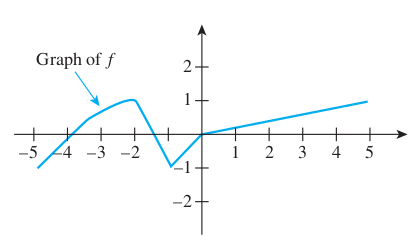
\includegraphics[scale=0.5]{../images/11.1.22.png}
\end{figure}

Let \(f\) be the function whose graph follows. Sketch the graph of \(3f\).

\begin{proof}
\begin{figure}[ht!]
\centering
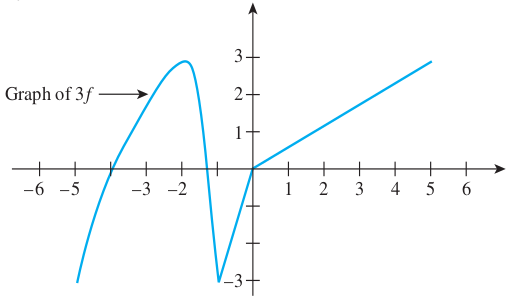
\includegraphics[scale=0.5]{../images/11.1.22.2.png}
\end{figure}
\end{proof}

\subsection{Exercise 23}
\begin{figure}[ht!]
\centering
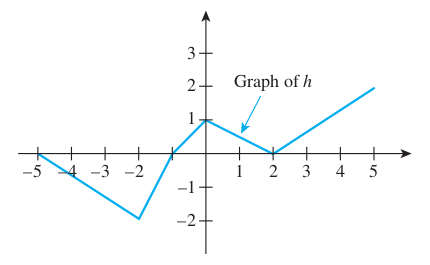
\includegraphics[scale=0.5]{../images/11.1.23.png}
\end{figure}

Let \(h\) be the function whose graph is shown above. Sketch the graph of \(2h\).

\begin{proof}
\begin{figure}[ht!]
\centering
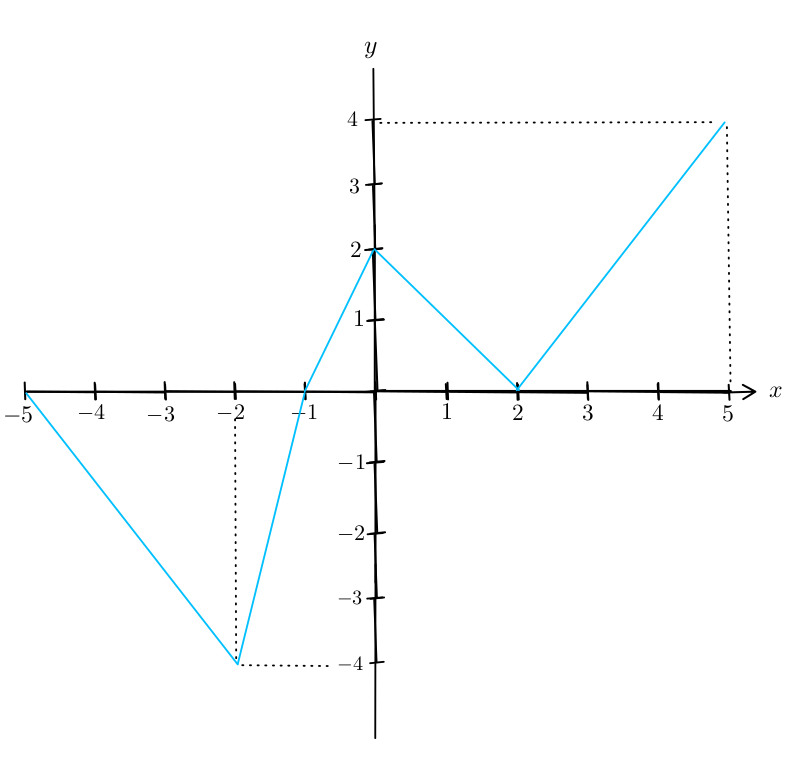
\includegraphics[scale=0.3]{../images/11.1.23.2.png}
\end{figure}
\end{proof}

\subsection{Exercise 24}
Let \(f\) be a real-valued function of a real variable. Show that if \(f\) is decreasing on a set \(S\) and if \(M\) is any 
positive real number, then \(Mf\) is decreasing on \(S\).

\begin{proof}
Suppose that \(f\) is a real-valued function of a real variable, \(f\) is decreasing on a set \(S\), and \(M\) is any 
positive real number. {\it [We must show that \(Mf\) is decreasing on \(S\). In other words, we must show that for all 
\(x_1\) and \(x_2\) in \(S\), if \(x_1 < x_2\) then \((Mf)(x_1) > (Mf)(x_2)\).]} Suppose \(x_1\) and \(x_2\) are in 
\(S\) and \(x_1 < x_2\). Since \(f\) is decreasing on \(S\), \(f(x_1) > f(x_2)\), and since \(M\) is positive, \(Mf(x_1) >
Mf(x_2)\) {\it [because when both sides of an inequality are multiplied by a positive number, the direction of the 
inequality is unchanged].} It follows by definition of \(Mf\) that \((Mf)(x_1) > (Mf)(x_2)\), {\it [as was to be shown].}
\end{proof}

\subsection{Exercise 25}
Let \(f\) be a real-valued function of a real variable. Show that if \(f\) is increasing on a set \(S\) and if \(M\) is any 
negative real number, then \(Mf\) is decreasing on \(S\).

\begin{proof}
The proof is the same as in Exercise 24, except that this time we have \(f(x_1) < f(x_2)\) because \(f\) is increasing, and 
multiplying an inequality by a negative number \(M\) reverses
the direction of the equality, so \(Mf(x_1) > Mf(x_2)\).
\end{proof}

\subsection{Exercise 26}
Let \(f\) be a real-valued function of a real variable. Show that if \(f\) is decreasing on a set \(S\) and if \(M\) is any 
negative real number, then \(Mf\) is increasing on \(S\).

\begin{proof}
The proof is the same as in Exercise 24, except that this time 
multiplying an inequality by a negative number \(M\) reverses
the direction of the equality, so \(Mf(x_1) < Mf(x_2)\).
\end{proof}

{\bf \cy In 27 and 28, functions \(f\) and \(g\) are defined. In each case sketch the graphs of \(f\) and \(2g\) on the same 
set of axes and find a number \(x_0\) so that \(f(x) \leq 2g(x)\) for all \(x > x_0\). You can find an exact value for 
\(x_0\) by solving a quadratic equation, or you can find an approximate value for \(x_0\) by using a graphing calculator 
or computer.}

\subsection{Exercise 27}
\(f(x) = x^2 + 10x + 11\) and \(g(x) = x^2\) for each real number \(x \geq 0\)

\begin{proof}
\begin{figure}[ht!]
\centering
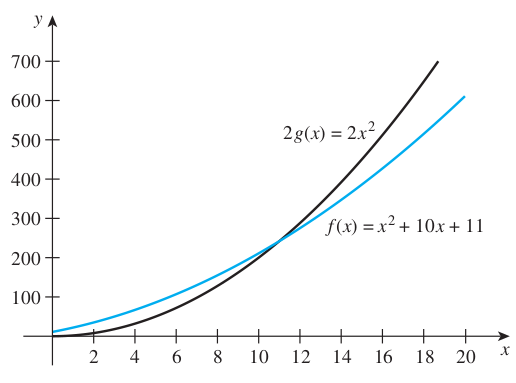
\includegraphics[scale=0.5]{../images/11.1.27.png}
\end{figure}

To find the answer algebraically, solve the equation \(2x^2 = x^2 + 10x + 11\) for \(x\). Subtracting \(x^2\) from both 
sides gives \(x^2 - 10x - 11 = 0\), and either using the quadratic formula or factoring \(x^2-10x-11=(x - 11)(x + 1)\) 
gives \(x = 11\) (since \(x > 0\)). To find an approximate answer with a graphing calculator, plot both \(f(x) = x^2 + 
10x + 11\) and \(2g(x) = 2x^2\) for \(x > 0\), as shown in the figure, and find that \(2g(x) > f(x)\) when \(x > 11\) 
(approximately). You can obtain only an approximate answer from a graphing calculator because the calculator computes 
values only to an accuracy of a finite number of decimal places.
\end{proof}

\subsection{Exercise 28}
\(f(x) = x^2 + 125x + 254\) and \(g(x) = x^2\) for each real number \(x \geq 0\)

\begin{proof}
\begin{figure}[ht!]
\centering
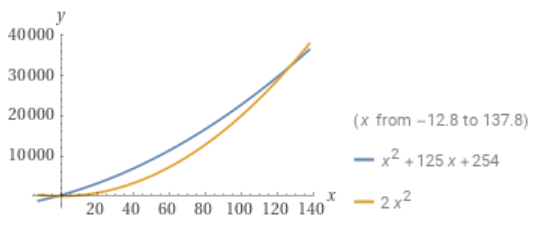
\includegraphics[scale=0.5]{../images/11.1.28.png}
\end{figure}

If we set \(f(x) = 2g(x)\) and solve, we get \(x^2 + 125x + 254 = 2x^2\) which gives \(x^2 - 125x - 254 = 0\) which 
factors as \((x-127)(x+2) = 0\) which has solutions \(x = -2, 127\). So let \(x_0 = 127\), so that \(f(x) < g(x)\) for all
\(x > x_0 = 127\).
\end{proof}

\section{Exercise Set 11.2}

\subsection{Exercise 1}
The following is a formal definition for \(\Omega\)-notation, written using quantifiers and variables: \(f(n)\) is \(\Omega 
(g(n))\) if, and only if, \(\te\) positive real numbers \(a\) and \(A\) such that \(\fa n \geq a, Ag(n) \leq f(n)\).

\subsubsection{(a)}
Write the formal negation for the definition using the symbols \(\fa\) and \(\te\).

\begin{proof}
Formal version of negation: \(f(n)\) is not \(\Omega(g(n))\) if, and only if, \(\fa\) positive real numbers \(a\) and 
\(A\), \(\te\) an integer \(n \geq a\) such that \(Ag(n) > f(n)\).
\end{proof}

\subsubsection{(b)}
Restate the negation less formally without using the symbols \(\fa\) and \(\te\) or the words “for any,” “for every,” or 
“there exists.”

\begin{proof}
Informal version of negation: \(f(n)\) is not \(\Omega(g(n))\) if, and only if, no matter what positive real numbers \(a\) 
and \(A\) might be chosen, it is possible to find an integer \(n\) greater than or equal to \(a\) with the property that 
\(Ag(n) > f(n)\).
\end{proof}

\subsection{Exercise 2}
The following is a formal definition for \(O\)-notation, written using quantifiers and variables: \(f(n)\) is 
\(O(g(n))\) if, and only if, \(\te\) positive real numbers \(b\) and \(B\) such that \(\fa n \geq b\), 
\(0 \leq f(n) \leq Bg(n)\).

\subsubsection{(a)}
Write the formal negation for the definition using the symbols \(\fa\) and \(\te\).

\begin{proof}
\(f(n)\) is not \(O(g(n))\) if, and only if, \(\fa\) positive real numbers \(b\) and \(B\), \(\te n \geq b\) such that 
\(0 > f(n)\) or \(f(n) > Bg(n)\).
\end{proof}

\subsubsection{(b)}
Restate the negation less formally without using the symbols \(\fa\) and \(\te\) or the words “for any,” “for every,” or 
“there exists.”

\begin{proof}
\(f(n)\) is not \(O(g(n))\) if, and only if, no matter what positive real numbers \(b\) and \(B\) are chosen, it is 
possible to choose an integer \(n\) greater than \(b\) with the property that either \(0 > f(n)\) or \(f(n) > Bg(n)\).
\end{proof}

\subsection{Exercise 3}
The following is a formal definition for \(\Theta\)-notation, written using quantifiers and variables: \(f(n)\) is \(\Theta 
(g(n))\) if, and only if, \(\te\) positive real numbers \(k, A\) and \(B\) such that \(\fa n \geq b, Ag(n) \leq f(n) \leq 
Bg(n)\).


\subsubsection{(a)}
Write the formal negation for the definition using the symbols \(\fa\) and \(\te\).

\begin{proof}
\(f(n)\) is not \(\Theta(g(n))\) if, and only if, \(\fa\) positive real numbers \(k, A\) and \(B\), \(\te n \geq b\) such that \(Ag(n) > f(n)\) or \(f(n) > Bg(n)\).
\end{proof}

\subsubsection{(b)}
Restate the negation less formally without using the symbols \(\fa\) and \(\te\) or the words “for any,” “for every,” or 
“there exists.”

\begin{proof}
\(f(n)\) is not \(\Theta(g(n))\) if, and only if, no matter what positive real numbers \(k, A\) and \(B\) are chosen, it 
is possible to choose an integer \(n\) greater than \(b\) with the property that either \(Ag(n) > f(n)\) or \(f(n) > Bg(n)\).
\end{proof}

{\bf \cy In \(4-9\), express each statement using \(\Omega\)-, \(O\)-, or \(\Theta\)-notation.}

\subsection{Exercise 4}
\(\dps \frac{1}{2}n \leq n - \floor{\frac{n}{2}} + 1\) for every integer \(n \geq 1\). (Use \(\Omega\)-notation).

\begin{proof}
\(\dps n - \floor{\frac{n}{2}} + 1\) is \(\Omega(n)\)
\end{proof}

\subsection{Exercise 5}
\(\dps 0 \leq n - \floor{\frac{n}{2}} + 1 \leq n\) for every integer \(n \geq 3\). (Use \(O\)-notation).

\begin{proof}
\(\dps n - \floor{\frac{n}{2}} + 1\) is \(O(n)\)
\end{proof}

\subsection{Exercise 6}
\(n^2 \leq 3n(n - 2) \leq 4n^2\) for every integer \(n \geq 3\). (Use \(\Theta\)-notation.)

\begin{proof}
\(3n(n - 2)\) is \(\Theta(n^2)\)
\end{proof}

\subsection{Exercise 7}
\(\dps \frac{1}{2}n^2 \leq \frac{n(3n-2)}{2}\) for every integer \(n \geq 3\). (Use \(\Omega\)-notation).

\begin{proof}
\(\dps \frac{n(3n-2)}{2}\) is \(\Omega(n^2)\)
\end{proof}

\subsection{Exercise 8}
\(\dps 0 \leq \frac{n(3n-2)}{2} \leq n^2\) for every integer \(n \geq 1\). (Use \(O\)-notation).

\begin{proof}
\(\dps \frac{n(3n-2)}{2}\) is \(O(n^2)\)
\end{proof}

\subsection{Exercise 9}
\(\dps \frac{n^3}{6} \leq n^2 \left(\ceil{\frac{n}{3}} - 1\right) \leq n^3\) for every integer \(n \geq 2\). 
(Use \(\Theta\)-notation.)

\begin{proof}
\(\dps n^2\left(\ceil{\frac{n}{3}} - 1\right)\) is \(\Theta(n^3)\)
\end{proof}

\subsection{Exercise 10}
\subsubsection{(a)}
Show that for any integer \(n \geq 1, 0 \leq 2n^2 + 15n + 4 \leq 21n^2\).

\begin{proof}
For each integer \(n \geq 1, 0 \leq 2n^2 + 15n + 4\) because all terms in \(2n^2 + 15n + 4\) are positive. Moreover, 
\(2n^2 + 15n + 4 \leq 2n^2 + 15n^2 + 4n^2\) because when \(n \geq 1\), \(15n \leq 15n^2\) and \(4 \leq 4n^2\), which add up 
to \(21n^2\) by combining like terms. Therefore, by transitivity of equality and order, \(0 \leq 2n^2 + 15n + 4 
\leq 21n^2\) for each integer \(n \geq 1\).
\end{proof}

\subsubsection{(b)}
Show that for any integer \(n \geq 1, 2n^2 \leq 2n^2 + 15n + 4\).

\begin{proof}
For each integer \(n \geq 1, 2n^2 \leq 2n^2 + 15n + 4\) because \(15n + 4 > 0\) since \(n\) is positive.
\end{proof}

\subsubsection{(c)}
Sketch a graph to illustrate the results of parts (a) and (b).
\begin{proof}
\begin{figure}[ht!]
\centering
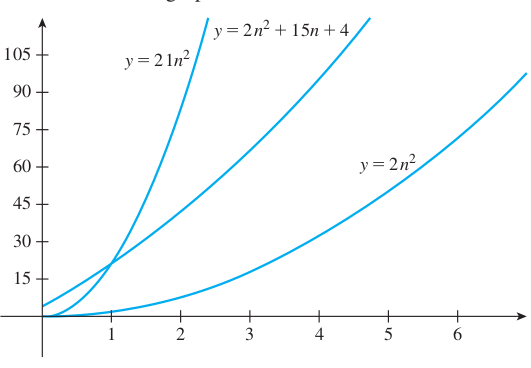
\includegraphics[scale=0.5]{../images/11.2.10.c.png}
\end{figure}
\end{proof}

\subsubsection{(d)}
Use the \(O\)- and \(\Omega\)-notations to express the results of parts (a) and (b).

\begin{proof}
Let \(A = 2\) and \(a = 1\). Then, by substitution from the result of part (b), \(An^2 < 2n^2 + 15n + 4\) for each integer 
\(n \geq a\), and hence, by definition of \(\Omega\)-notation, \(2n^2 + 15n + 4\) is \(\Omega(n^2)\). Let \(B = 21\) and 
\(b = 1\). Then, by substitution from the result of part (a), \(0< 2n^2 + 15n + 4 \leq Bn^2\) for each integer \(n \geq b\), 
and hence by definition of \(O\)-notation, \(2n^2 + 15n + 4\) is \(O(n^2)\).
\end{proof}

\subsubsection{(e)}
What can you deduce about the order of \(2n^2 + 15n + 4\)?
\begin{proof}
{\it Solution 1:} Let \(A = 2, B = 21\), and \(k = 1\). By the results of parts (a) and (b), \(An^2 \leq 2n^2 + 15n + 4 \leq 
Bn^2\) for each integer \(n \geq k\), and hence, by definition of \(\Theta\)-notation, \(2n^2 + 15n + 4\) is \(\Theta(n^2)\).

{\it Solution 2:} By part (d), \(2n^2 + 15n + 4\) is both \(\Omega(n^2)\) and \(O(n^2)\). Hence, by Theorem 11.2.1, 
\(2n^2 + 15n + 4\) is \(\Theta(n^2)\).
\end{proof}

\subsection{Exercise 11}
\subsubsection{(a)}
Show that for any integer \(n \geq 1, 0 \leq 23n^4 + 8n^2 + 4n \leq 35n^4\).

\begin{proof}
For each integer \(n \geq 1, 0 \leq 23n^4 + 8n^2 + 4n\) because all terms in \(23n^4 + 8n^2 + 4n\) are positive. 
Moreover, \(23n^4 + 8n^2 + 4n \leq 23n^4 + 8n^4 + 4n^4\) because when \(n \geq 1\), \(8n^2 \leq 8n^4\) and 
\(4n \leq 4n^4\), which add up to \(35n^4\) by combining like terms. Therefore, by transitivity of equality and order, 
\(0 \leq 23n^4 + 8n^2 + 4n \leq 35n^4\) for each integer \(n \geq 1\).
\end{proof}

\subsubsection{(b)}
Show that for any integer \(n \geq 1, 23n^4 \leq 23n^4 + 8n^2 + 4n\).

\begin{proof}
For each integer \(n \geq 1, 23n^4 \leq 23n^4 + 8n^2 + 4n\) because \(8n^2 + 4n > 0\) since \(n\) is positive.
\end{proof}

\subsubsection{(c)}
Sketch a graph to illustrate the results of parts (a) and (b).
\begin{proof}
\begin{figure}[ht!]
\centering
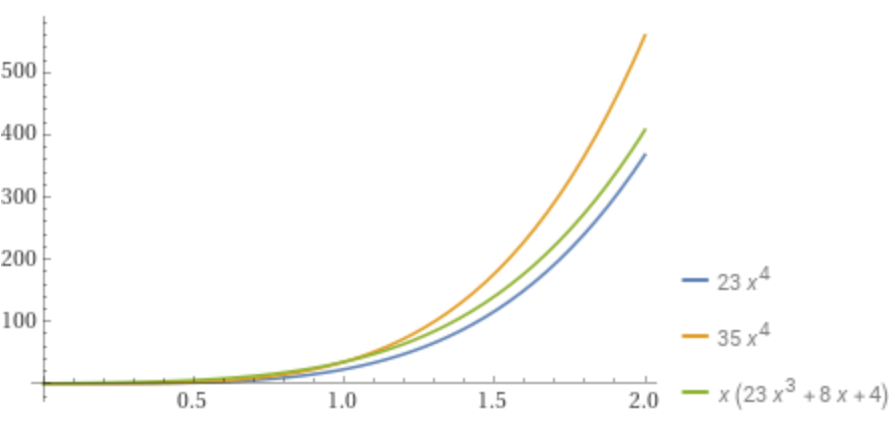
\includegraphics[scale=0.5]{../images/11.2.11.c.png}
\end{figure}
\end{proof}

\subsubsection{(d)}
Use the \(O\)- and \(\Omega\)-notations to express the results of parts (a) and (b).

\begin{proof}
Let \(A = 23\) and \(a = 1\). Then, by substitution from the result of part (b), \(An^4 < 23n^4 + 8n^2 + 4n\) for each 
integer \(n \geq a\), and hence, by definition of \(\Omega\)-notation, \(23n^4 + 8n^2 + 4n\) is \(\Omega(n^4)\). Let 
\(B = 35\) and \(b = 1\). Then, by substitution from the result of part (a), \(0 < 23n^4 + 8n^2 + 4n \leq Bn^4\) for 
each integer \(n \geq b\), and hence by definition of \(O\)-notation, \(23n^4 + 8n^2 + 4n\) is \(O(n^4)\).
\end{proof}

\subsubsection{(e)}
What can you deduce about the order of \(23n^4 + 8n^2 + 4n\)?
\begin{proof}
By part (d), \(23n^4 + 8n^2 + 4n\) is both \(\Omega(n^4)\) and \(O(n^4)\). Hence, by Theorem 11.2.1, \(23n^4 + 8n^2 + 4n\) is 
\(\Theta(n^4)\).
\end{proof}

\subsection{Exercise 12}
\subsubsection{(a)}
Show that for any integer \(n \geq 1, 0 \leq 7n^3 + 10n^2 + 3 \leq 20n^3\).

\begin{proof}
For each integer \(n \geq 1, 0 \leq 7n^3 + 10n^2 + 3\) because all terms in \(7n^3 + 10n^2 + 3\) are positive. Moreover, 
\(7n^3 + 10n^2 + 3 \leq 7n^3 + 10n^3 + 3n^3\) because when \(n \geq 1\), \(10n^2 \leq 10n^3\) and \(3 \leq 3n^3\), which add 
up to \(20n^3\) by combining like terms. Therefore, by transitivity of equality and order, \(0 \leq 7n^3 + 10n^2 + 3 
\leq 20n^3\) for each integer \(n \geq 1\).
\end{proof}

\subsubsection{(b)}
Show that for any integer \(n \geq 1, 7n^3 \leq 7n^3 + 10n^2 + 3\).

\begin{proof}
For each integer \(n \geq 1, 7n^3 \leq 7n^3 + 10n^2 + 3\) because \(10n^2 + 3 > 0\) since \(n\) is positive.
\end{proof}

\subsubsection{(c)}
Sketch a graph to illustrate the results of parts (a) and (b).
\begin{proof}
\begin{figure}[ht!]
\centering
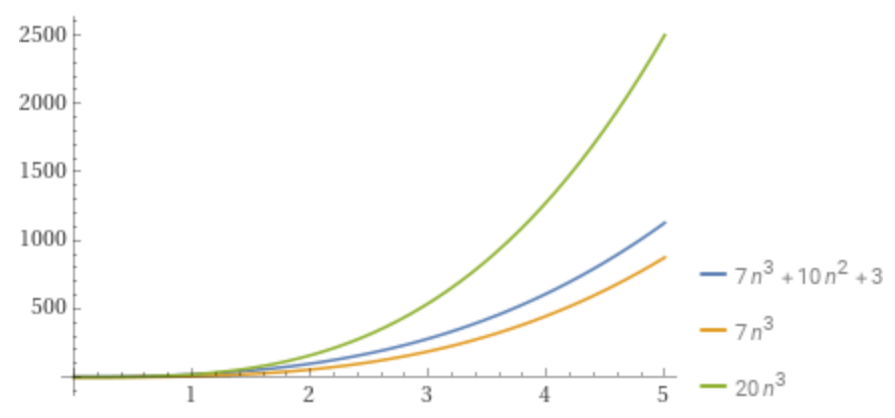
\includegraphics[scale=0.5]{../images/11.2.12.c.png}
\end{figure}
\end{proof}

\subsubsection{(d)}
Use the \(O\)- and \(\Omega\)-notations to express the results of parts (a) and (b).

\begin{proof}
Let \(A = 7\) and \(a = 1\). Then, by substitution from the result of part (b), \(An^3 < 7n^3 + 10n^2 + 3\) for each 
integer \(n \geq a\), and hence, by definition of \(\Omega\)-notation, \(7n^3 + 10n^2 + 3\) is \(\Omega(n^3)\). Let 
\(B = 20\) and \(b = 1\). Then, by substitution from the result of part (a), \(0 < 7n^3 + 10n^2 + 3 \leq Bn^3\) for 
each integer \(n \geq b\), and hence by definition of \(O\)-notation, \(7n^3 + 10n^2 + 3\) is \(O(n^3)\).
\end{proof}

\subsubsection{(e)}
What can you deduce about the order of \(7n^3 + 10n^2 + 3\)?
\begin{proof}
By part (d), \(7n^3 + 10n^2 + 3\) is both \(\Omega(n^3)\) and \(O(n^3)\). Hence, by Theorem 11.2.1, \(7n^3 + 10n^2 + 3\) is 
\(\Theta(n^3)\).
\end{proof}

\subsection{Exercise 13}
Use the definition of \(\Theta\)-notation to show that \(5n^3 + 65n + 30\) is \(\Theta(n^3)\).

\begin{proof}
For each integer \(n \geq 1\), \(5n^3 \leq 5n^3 + 65n + 30\) because \(65n + 30 > 0\) since \(n\) is positive. Moreover, 
\(5n^3 + 65n + 30 \leq 5n^3 + 65n^3 + 30n^3\) because when \(n \geq 1\), then \(65n < 65n^3\) and \(30 < 30n^3\), which add 
up to \(100n^3\) by combining like terms. Therefore, by transitivity of order and equality, \(5n^3 \leq 5n^3 + 65n + 
30 \leq 100n^3\). Thus, let \(A = 5, B = 100\), and \(k = 1\). Then \(An^3 \leq 5n^3 + 65n + 30 \leq Bn^3\) for each integer 
\(n \geq k\), and hence, by definition of \(\Theta\)-notation, \(5n^3 + 65n + 30\) is \(\Theta(n^3)\).
\end{proof}

\subsection{Exercise 14}
Use the definition of \(\Theta\)-notation to show that \(n^2 + 100n + 88\) is \(\Theta(n^2)\).

\begin{proof}
For each integer \(n \geq 1\), \(n^2 \leq n^2 + 100n + 88\) because \(100n + 88 > 0\) since \(n\) is positive. Moreover, 
\(n^2 + 100n + 88 \leq n^2 + 100n^2 + 88n^2\) because when \(n \geq 1\), then \(100n < 100n^2\) and \(88 < 88n^2\), which add 
up to \(189n^2\) by combining like terms. Therefore, by transitivity of order and equality, \(n^2 \leq n^2 + 100n + 88 \leq 189n^2\). Thus, let \(A = 1, B = 189\), and \(k = 1\). Then \(An^2 \leq n^2 + 100n + 88 \leq Bn^2\) for each integer 
\(n \geq k\), and hence, by definition of \(\Theta\)-notation, \(n^2 + 100n + 88\) is \(\Theta(n^2)\).
\end{proof}

\subsection{Exercise 15}
Use the definition of \(\Theta\)-notation to show that \(\dps \floor{n + \frac{1}{2}}\) is \(\Theta(n)\).

\begin{proof}
For each integer \(n \geq 1\), \(\dps n \leq n + \frac{1}{2} < n+1\), and so by definition of floor, \(\dps \floor{n + 
\frac{1}{2}} = n\), and \(\dps \floor{n + \frac{1}{2}}\) is nonnegative. In addition, when \(n \geq 1\), then \(n + 1 \leq 
n + n = 2n\), and thus, by transitivity of equality and order, \(\dps n \leq \floor{n + \frac{1}{2}} \leq 2n\).
Let \(A = 1, B = 2\), and \(k = 1\). Then \(\dps An\leq \floor {n+\frac{1}{2}}\leq Bn\) for every integer \(n \geq k\),
and hence, by definition of \(\Theta\)-notation, \(\dps \floor {n+\frac{1}{2}}\) is \(\Theta(n)\).
\end{proof}

\subsection{Exercise 16}
Use the definition of \(\Theta\)-notation to show that \(\dps \ceil{n + \frac{1}{2}}\) is \(\Theta(n)\).

\begin{proof}
For each integer \(n \geq 1\), \(\dps n < n + \frac{1}{2} \leq n+1\), and so by definition of ceiling, \(\dps \ceil{n + 
\frac{1}{2}} = n+1\), and \(\dps \ceil{n + \frac{1}{2}}\) is nonnegative. In addition, when \(n \geq 1\), then \(n + 1 \leq 
n + n = 2n\), and thus, by transitivity of equality and order, \(\dps n < \ceil{n + \frac{1}{2}} \leq 2n\).
Let \(A = 1, B = 2\), and \(k = 1\). Then \(\dps An\leq \ceil{n+\frac{1}{2}}\leq Bn\) for every integer \(n \geq k\),
and hence, by definition of \(\Theta\)-notation, \(\dps \ceil {n+\frac{1}{2}}\) is \(\Theta(n)\).
\end{proof}

\subsection{Exercise 17}
Use the definition of \(\Theta\)-notation to show that \(\dps \floor{\frac{n}{2}}\) is \(\Theta(n)\). ({\it Hint:} Show 
that if \(n \geq 4\), then \(\dps \frac{n}{2} - 1 \geq \frac{1}{4}n\).)

\begin{proof}
Assume \(n \geq 2\) is even. 

Then \(n = 2k\) for some integer \(k\) and thus \(\dps \floor{\frac{n}{2}} = \floor{\frac{2k}{2}} = \floor{k} = 
\frac{n}{2}\). Then notice that \(\dps \frac{1}{4}n \leq \frac{n}{2} \leq n\). So \(\dps \frac{1}{4}n \leq 
\floor{\frac{n}{2}} \leq n\).

Now assume \(n \geq 2\) is odd. 

Then \(n = 2k+1\) for some integer \(k\) and thus \(\dps \floor{\frac{n}{2}} = \floor{\frac{2k+1}{2}} = \floor{k + 
\frac{1}{2}} = k = \frac{n-1}{2}\). Now \(n-1 \leq n \leq 2n\), so \(\dps \frac{n-1}{2} \leq n\). And \(2 \leq n\) 
implies \(0 \leq n-2\) so \(n \leq 2n - 2\) then \(\dps \frac{1}{4}n \leq \frac{2n-2}{4} = \frac{n-1}{2}\). Thus 
\(\dps \frac{1}{4}n \leq \floor{\frac{n}{2}} \leq n\).

So, in all cases, for \(n \geq 2\) we have \(\dps \frac{1}{4}n \leq \floor{\frac{n}{2}} \leq n\). Let \(A = \frac{1}{4},
B = 1, k = 2\). Then for all \(\dps n \geq k, An \leq \floor{\frac{n}{2}} \leq Bn\). So by definition of \(\Theta\)
notation, \(\dps \floor{\frac{n}{2}}\) is \(\Theta(n)\).
\end{proof}

\subsection{Exercise 18}
Prove Theorem 11.2.7(b): If \(f\) and \(g\) are real-valued functions defined on the same set of nonnegative integers and 
if \(f(n) \geq 0\) and \(g(n) \geq 0\) for every integer \(n \geq r\), where \(r\) is a positive real number, then if 
\(f(n)\) is \(\Theta(g(n))\), then \(g(n)\) is \(\Theta(f(n))\).

\begin{proof}
Suppose \(f\) and \(g\) are real-valued functions defined on the same set of nonnegative integers, suppose \(f(n) \geq 0\) 
and \(g(n) \geq 0\) for every integer \(n \geq r\), where \(r\) is a positive real number, and suppose \(f(n)\) is 
\(\Theta(g(n))\). {\it [We must show that \(g(n)\) is \(\Theta(f(n))\).]} By definition of \(\Theta\)-notation, there
exist positive real numbers \(A, B\), and \(k\) with \(k \geq r\) such that for each integer \(n \geq k, Ag(n) \leq f(n) 
\leq Bg(n)\). Dividing the left-hand inequality by \(A\) and the right-hand inequality by \(B\) gives that \(g(n) \leq 
\frac{1}{A}f(n)\) and \(\frac{1}{B}f(n) \leq g(n)\), and combining the resulting inequalities produces \(\frac{1}{B}
f(n) \leq g(n) \leq \frac{1}{A}f(n)\) for each integer \(n \geq k\). Now both \(f(n) \geq 0\) and \(g(n) \geq 0\) for 
each integer \(n \geq k\). Also, since both \(A\) and \(B\) are positive real numbers, so are \(1/A\) and \(1/B\). Thus, 
by definition of \(\Theta\)-notation, \(g(n)\) is \(\Theta (f(n))\).
\end{proof}

\subsection{Exercise 19}
Prove Theorem 11.2.1: If \(f\) and \(g\) are real-valued functions defined on the same set of nonnegative integers and 
if \(f(n) \geq 0\) and \(g(n) \geq 0\) for every integer \(n \geq r\), where \(r\) is a positive real number, then \(f(n)\) 
is \(\Theta(g(n))\) if, and only if, \(f(n)\) is \(\Omega(g(n))\) and \(f(n)\) is \(O(g(n))\).

\begin{proof}
Assume \(f(n) \geq 0\) and \(g(n) \geq 0\) for every integer \(n \geq r > 0\).

\(\bm{(\implies)}\) 1. Assume \(f(n)\) is \(\Theta(g(n))\).

2. By definition of \(\Theta\)-notation, there exist positive real numbers \(A, B\), and \(k \geq r\) such that \(A g(n) 
\leq f(n) \leq B g(n)\) for every integer \(n \geq k\).

3. By 2 and assumption, \(0 \leq f(n) \leq Bg(n)\) for all \(n \geq k\), so by definition of \(O\)-notation, \(f(n)\) is 
\(O(g(n))\).

4. By 2, \(Ag(n) \leq f(n)\) for all \(n \geq k\), so by definition of \(\Omega\)-notation, \(f(n)\) is \(\Omega(g(n))\).

\(\bm{(\impliedby)}\) 1. Assume \(f(n)\) is \(\Omega(g(n))\) and \(f(n)\) is \(O(g(n))\).

2. By 1 and definition of \(\Omega\)-notation, there exist positive real numbers \(A\) and \(a \geq r\) such that 
\(Ag(n) \leq f(n)\) for every integer \(n \geq a\).

3. By 1 and definition of \(O\)-notation, there exist positive real numbers \(B\) and \(b \geq r\) such that 
\(0 \leq f(n) \leq Bg(n)\) for every integer \(n \geq b\).

4. Let \(c = max(a,b)\). Then by 2 and 3, for every \(n \geq c\), \(Ag(n) \leq f(n) \leq Bg(n)\). So by definition of 
\(\Theta\)-notation, \(f(n)\) is \(\Theta(g(n))\).
\end{proof}

\subsection{Exercise 20}
Without using Theorem 11.2.4 prove that \(n^5\) is not \(O(n^2)\).

\begin{proof}
Suppose not. That is, suppose \(n^5\) is \(O(n^2)\). {\it [We must show that this supposition leads to a contradiction.]} By 
definition of \(O\)-notation, there exist positive real numbers \(B\) and \(b\) such that \(0 \leq n^5 \leq Bn^2\) for 
each integer \(n \geq b\). Dividing the inequalities by \(n^2\) and taking the cube root of both sides gives 
\(0 \leq n \leq \sqrt[3]{B}\) for each integer \(n \geq b\). These two conditions are contradictory because on the one hand 
\(n\) can be any integer greater than or equal to \(b\), but when \(n\) is greater than \(b\), then \(n\) is less than 
\(\sqrt[3]{B}\), which is a fixed integer. Thus the supposition leads to a contradiction, and hence the 
supposition is false.
\end{proof}

\subsection{Exercise 21}
Prove Theorem 11.2.4: If \(f\) is a real-valued function defined on a set of nonnegative integers and \(f(n)\) is 
\(\Omega(n^m)\), where \(m\) is a positive integer, then \(f(n)\) is not \(O(n^p)\) for any positive real number 
\(p < m\).

\begin{proof}
Assume \(m\) is a positive integer, \(p\) is a positive real number, \(p < m\) and \(f(n)\) is \(\Omega(n^m)\). 

By definition of \(\Omega\)-notation there exist positive real numbers \(A\) and \(a \geq 0\) such that \(An^m \leq f(n)\) 
for every integer \(n \geq a\). (We are taking \(r = 0\) since \(n^m \geq 0\) for all \(n \geq 0\).)

Argue by contradiction and assume \(f(n)\) is \(O(n^p)\). By definition of \(O\)-notation, there exist positive real 
numbers \(B\) and \(b \geq r\) such that \(0 \leq f(n) \leq Bn^p\) for every integer \(n \geq b\).

Let \(c = max(a, b)\). Then for all \(n \geq c\) we have \(An^m \leq f(n) \leq Bn^p\). In particular, \(An^m \leq Bn^p\)
for all \(n \geq c\). Dividing by \(An^p\) we get \(\dps n^{m-p} \leq \frac{B}{A}\) for all \(n \geq c\). Since \(m-p > 0\),
this is a contradiction: the left hand side is a function that grows without bound as \(n\) gets larger, and the right hand
side is a positive constant.

So our supposition was false, and \(f(n)\) is not \(O(n^p)\).
\end{proof}

\subsection{Exercise 22}
\subsubsection{(a)}
Use one of the methods of Example 11.2.4 to show that \(2n^4 - 90n^3 + 3\) is \(\Omega(n^4)\).

\begin{proof}
To use the general procedure from Example 11.2.4 to show that \(2n^4 - 90n^3 + 3\) is \(\Omega(n^4)\), let \(A = \frac{1}{2} 
\cdot 2 = 1\) and \(a = \frac{2}{2}(|-90| + |3|) = 93\) and note that \(a \geq 1\). We will show that \(n^4 \leq 2n^4 -
90n^3 + 3\) for every integer \(n \geq a\). Now \(n \geq a\) means that \(n \geq 90+3\). Multiplying both sides by \(n^3\) 
gives \(n^4 \geq 90n^3 + 3n^3\) and subtracting first \(3n^3\) and then 3 from the right-hand side gives that \(n^4 \geq 
90n^3 \geq 90n^3 - 3\) for every integer \(n \geq a\). Subtracting the right-hand side from the left-hand side and 
adding \(n^4\) to both sides gives \(2n^4 - 90n^3 + 3 \geq n^4\) for every integer \(n \geq a\). Thus since \(A = 1\), 
\(2n^4 - 90n^3 + 3 \geq An^4\) for every integer \(n \geq a\), and so, by definition of \(\Omega\)-notation, 
\(2n^4 - 90n^3 + 3\) is \(\Omega(n^4)\).
\end{proof}

\subsubsection{(b)}
Show that \(2n^4 - 90n^3 + 3\) is \(O(n^4)\).
\begin{proof}
To show that \(2n^4 - 90n^3 + 3\) is \(O(n^4)\), observe that for every integer \(n \geq 1\), 
\(2n^4 - 90n^3 + 3 \leq 2n^4 + 90n^3 + 3\) because when \(n \geq 1\), then \(90n^3\) is positive, 

\(\leq 2n^4 + 90n^4 + 3n^4\) by Theorem 11.2.2 (since \(n \geq 1\), \(n^3 \leq n^4\) and \(1 \leq n^4\), \(90n^3 \leq 90n^4\) 
and \(3 \leq 3n^4\)),

and so \(= 95n^4\) because \(2 + 90 + 3 = 95\). Thus, by transitivity of order and equality, for every integer 
\(n \geq 1\), \(2n^4 - 90n^3 + 3 \leq 95n^4\). 

In addition, by part (a), for every integer \(n \geq 60\), \(\frac{1}{2}n^4 \leq 2n^4 - 90n^3 + 3\) so since 
\(0 \leq 12 n^4\), transitivity of order gives that for every integer \(n \geq 60\), \(0 \leq 2n^4 - 90n^3 + 3 \leq 95n^4\). 

Let \(B = 14\) and \(b = 60\). Then, for every integer \(n \geq b\), \(0 \leq 2n^4 - 90n^3 + 3 \leq Bn^4\) and hence, by 
definition of \(O\)-notation, \(2n^4 - 90n^3 + 3\) is \(O(n^4)\).
\end{proof}

\subsubsection{(c)}
Justify the conclusion that \(2n^4 - 90n^3 + 3\) is \(\Theta(n^4)\).

\begin{proof}
By parts (a) and (b), \(2n^4 - 90n^3 + 3\) is both \(\Omega(n^4)\) and \(O(n^4)\). Hence, by Theorem 11.2.1, 
\(2n^4 - 90n^3 + 3\) is \(\Theta(n^4)\).
\end{proof}

\subsection{Exercise 23}
\subsubsection{(a)}
Use one of the methods of Example 11.2.4 to show that \(\frac{1}{5}n^2 - 42n - 8\) is \(\Omega(n^2)\).

\begin{proof}
Let \(\dps f(n) = \frac{1}{5}n^2 - 42n - 8\). 

To find the lower bound, let us follow the procedure. Let \(\dps A = \frac{1}{2} \cdot \frac{1}{5} = \frac{1}{10}\). 
Let \(\dps a = \frac{2}{1/5}(|-42| + |-8|) = 500\). Now we need to show that \(\dps \frac{1}{10}n^2 \leq f(n)\) for 
\(n \geq 500\).

Assume \(n \geq 500\), which means \(n \geq 10(42+8)\). Divide by 10 and multiply by \(n\) to get \(\dps \frac{1}{10}n^2 \geq 
42n + 8n\). Subtract \(8n-8\) from the right hand side to get \(42n + 8n \geq 42n + 8\) (because when \(n \geq 500\), 
\(8n - 8 \geq 0\), so subtracting a positive number makes it smaller). So by transitivity of order, \(\dps \frac{1}{10}n^2 
\geq 42n + 8\). Subtract right hand side from left hand side to get \(\dps \frac{1}{10}n^2 - 42n - 8 \geq 0\). Now add 
\(\dps \frac{1}{10}n^2\) to both sides to get \(\dps \frac{1}{5}n^2- 42n - 8 \geq \frac{1}{10}n^2\) for all \(n \geq 500\). 
So by definition of \(\Omega\)-notation, \(f(n)\) is \(\Omega(n^2)\).
\end{proof}

\subsubsection{(b)}
Show that \(\frac{1}{5}n^2 - 42n - 8\) is \(O(n^2)\).
\begin{proof}
Setting \(f(n) = 0\) we find 
\[
n = \frac{42 \pm \sqrt{(-42)^2-4(1/5)(-8)}}{2/5} = 105 \pm \sqrt{11065} \approx 0 \text{ and } 210,
\] 
so \(f(n) \geq 0\) for all \(n \geq 211\).

To find the upper bound, we can replace \(\frac{1}{5}n^2 - 42n - 8\) with the bigger \(n^2 + 42n^2 + 8n^2 = 51n^2\). So 
\(0 \leq f(n) \leq 51n^2\) for all \(n \geq 211\), so \(f(n)\) is \(O(n^2)\).
\end{proof}

\subsubsection{(c)}
Justify the conclusion that \(\frac{1}{5}n^2 - 42n - 8\) is \(\Theta(n^2)\).

\begin{proof}
By parts (a) and (b), \(f(n)\) is both \(\Omega(n^2)\) and \(O(n^2)\). By Theorem 11.2.1, \(f(n)\) is \(\Theta(n^2)\).
\end{proof}

\subsection{Exercise 24}
\subsubsection{(a)}
Use one of the methods of Example 11.2.4 to show that \(\frac{1}{4}n^5 - 50n^3 + 3n + 12\) is \(\Omega(n^5)\).

\begin{proof}
\(A = \frac{1}{2} \cdot \frac{1}{4} = \frac{1}{8}\), \(\dps a = \frac{2}{1/4}(|-50| + |3| + |12|) = 8(50 + 3 + 12)= 520\).

Assume \(n \geq 520 = 8(50+3+12)\). 

Divide by 8 and multiply by \(n^4\) to get \(\dps \frac{1}{8}n^5 \geq 50n^4 + 3n^4 + 12n^4\). 

From the right hand side, subtract \(50n^4 - 50n^3\) to get \(50n^4 + 3n^4 + 12n^4 \geq 50n^3 + 3n^4 + 12n^4\) (because
when \(n \geq 520\) we have \(12n^4 - 12n^3 = 12n^3(n-1) \geq 0\) so subtracting something positive makes it smaller).

From the right hand side, subtract \(3n^4 + 3n\) to get \(50n^3 + 3n^4 + 12n^4 \geq 50n^3 - 3n + 12n^4\) (because
when \(n \geq 520\) we have \(3n^4 + 3n = 3n(n^3+1) \geq 0\) so subtracting something positive makes it smaller).

From the right hand side, subtract \(12n^4 + 12\) to get \(50n^3 - 3n + 12n^4 \geq 50n^3 - 3n - 12\) (because when 
\(n \geq 520\) we have \(12n^4 + 12n = 12(n^4+1) \geq 0\) so subtracting something positive makes it smaller).

By transitivity of order we get \(\dps \frac{1}{8}n^5 \geq 50n^3 - 3n - 12\). Moving everything to the left hand side, we
get \(\dps \frac{1}{8}n^5 - 50n^3 + 3n + 12 \geq 0\). Now add \(\dps \frac{1}{8}n^5\) to both sides to finally get
\(\dps \frac{1}{4}n^5 - 50n^3 + 3n + 12 \geq \frac{1}{8}n^5\) for all \(n \geq 520\).

So by definition of \(\Omega\)-notation, \(f(n)\) is \(\Omega(n^5)\).
\end{proof}

\subsubsection{(b)}
Show that \(\frac{1}{4}n^5 - 50n^3 + 3n + 12\) is \(O(n^5)\).
\begin{proof}
Setting \(f(n) = 0\) we find \(n \approx -14, 1, 14\). So \(f(n) \geq 0\) for all \(n \geq 15\).

\(\frac{1}{4}n^5 - 50n^3 + 3n + 12 \leq n^5 + 50n^5 + 3n^5 + 12n^5 = 66n^5\) for all \(n \geq 1\).

Therefore \(0 \leq f(n) \leq 66n^5\) for all \(n \geq 15\). By definition of \(O\)-notation, \(f(n)\) is \(O(n^5)\).
\end{proof}

\subsubsection{(c)}
Justify the conclusion that \(\frac{1}{4}n^5 - 50n^3 + 3n + 12\) is \(\Theta(n^5)\).

\begin{proof}
By parts (a) and (b), \(f(n)\) is both \(\Omega(n^5)\) and \(O(n^5)\). By Theorem 11.2.1, \(f(n)\) is \(\Theta(n^5)\).
\end{proof}

\subsection{Exercise 25}
Suppose \(P(n) = a_mn^m + a_{m-1}n^{m-1} + \cdots + a_2n^2 + a_1n + a_0\), where all the coefficients \(a_0, a_1, \ldots, 
a_m\) are real numbers and \(a_m > 0\). 

\subsubsection{(a)}
Prove that \(P(n)\) is \(\Omega(n^m)\) by using the general procedure described in Example 11.2.4.

\begin{proof}
Let \(\dps A = \frac{1}{2}a_m\), \(\dps d = \frac{2}{a_m}(|a_{m-1}| + \cdots + |a_0|)\) and \(a = max(d, 1)\). Then 
\(n \geq a\) means that \(\dps n \geq \frac{2}{a_m}(|a_{m-1}| + \cdots + |a_0|)\). Multiplying both sides by \(\dps
\frac{1}{2}a_m n^{m-1}\) gives
\[
\frac{1}{2}a_m n^m \geq (|a_{m-1}| + \cdots + |a_0|)n^{m-1} = |a_{m-1}|n^{m-1} + |a_{m-2}|n^{m-1} + \cdots + |a_1|n^{m-1} +
|a_0|n^{m-1}
\]
which is \(\geq |a_{m-1}|n^{m-1} + |a_{m-2}|n^{m-2} + \cdots + |a_1|n^1 + |a_0|n^0\). So by transitivity of order
\[
\frac{1}{2}a_m n^m \geq |a_{m-1}|n^{m-1} + |a_{m-2}|n^{m-2} + \cdots + |a_1|n^1 + |a_0|n^0.
\]
Subtracting the right hand side gives
\[
\frac{1}{2}a_m n^m - |a_{m-1}|n^{m-1} - |a_{m-2}|n^{m-2} - \cdots - |a_1|n^1 - |a_0|n^0 \geq 0.
\]
Since each \(a_i \geq -|a_i|\), we have
\[
\frac{1}{2}a_m n^m + a_{m-1}n^{m-1} + \cdots + a_1n + a_0 \geq \frac{1}{2}a_m n^m - |a_{m-1}|n^{m-1} - \cdots - |a_1|n^1 - 
|a_0|n^0.
\]
By transitivity of order \(\frac{1}{2}a_m n^m + a_{m-1}n^{m-1} + \cdots + a_1n + a_0 \geq 0\). Add \(\frac{1}{2}a_mn^m\) to
both sides to get \(a_m n^m + a_{m-1}n^{m-1} + \cdots + a_1n + a_0 \geq \frac{1}{2}a_mn^m\). So by definition of \(\Omega\)
notation, \(P(n)\) is \(\Omega(n^m)\).
\end{proof}

\subsubsection{(b)}
Prove that \(P(n)\) is \(O(n^m)\).
\begin{proof}
For all \(n \geq 1\) we have \(a_mn^m + a_{m-1}n^{m-1} + \cdots + a_2n^2 + a_1n + a_0\) 

\(\leq |a_m|n^m + |a_{m-1}|n^m + \cdots + |a_2|n^m + |a_1|n^m + |a_0|n^m = (|a_m| + \cdots + |a_0|)n^m\).

Let \(B = |a_m| + \cdots + |a_0|\). Then, by transitivity of order and equality, for each integer \(n \geq 1\), \(a_mn^m + 
a_{m-1}n^{m-1} + \cdots + a_2n^2 + a_1n + a_0 \geq Bn^m\).

In addition, by part (a), there exists a positive real number \(a\) such that for each integer \(n \geq a\), \(\frac{a_m}{2}
n^m \leq a_mn^m + a_{m-1}n^{m-1} + \cdots + a_2n^2 + a_1n + a_0\).

Now \(\frac{a_n}{2} n^m > 0\) because \(a_m > 0\), and thus, transitivity of order gives that for each integer \(n\geq a\),
\(0 \leq a_mn^m + a_{m-1}n^{m-1} + \cdots + a_2n^2 + a_1n + a_0\).

And hence, by definition of \(O\)-notation, \(a_mn^m + a_{m-1}n^{m-1} + \cdots + a_2n^2 + a_1n + a_0\) is \(O(n^m)\).
\end{proof}

\subsubsection{(c)}
Justify the conclusion that \(P(n)\) is \(\Theta(n^m)\).
\begin{proof}
By parts (a) and (b), \(a_mn^m + a_{m-1}n^{m-1} + \cdots + a_2n^2 + a_1n + a_0\) is both \(\Omega(n^m)\) and \(O(n^m)\).
Hence, by Theorem 11.2.1, it is \(\Theta(n^m)\).
\end{proof}

{\bf \cy Use the theorem on polynomial orders to prove each of the statements in \(26-31\).}

\subsection{Exercise 26}
\(\dps \frac{(n+1)(n-2)}{4}\) is \(\Theta(n^2)\)

\begin{proof}
\(\dps \frac{(n+1)(n-2)}{4} = \frac{n^2-n-2}{4} = \frac{1}{4}n^2 - \frac{1}{4}n - \frac{1}{2}\), which is \(\Theta(n^2)\) 
by the theorem on polynomial orders.
\end{proof}

\subsection{Exercise 27}
\(\dps \frac{n}{3}(4n^2-1)\) is \(\Theta(n^3)\)

\begin{proof}
\(\dps \frac{n}{3}(4n^2-1) = \frac{4}{3}n^3 - \frac{1}{3}n\), which is \(\Theta(n^3)\) by the theorem on polynomial orders.
\end{proof}

\subsection{Exercise 28}
\(\dps \frac{n(n-1)}{2}+3n\) is \(\Theta(n^2)\)

\begin{proof}
\(\dps \frac{n(n-1)}{2}+3n = \frac{n^2-n}{2} + 3n = \frac{1}{2}n^2 + \frac{5}{2}n\), which is \(\Theta(n^2)\) by the 
theorem on polynomial orders.
\end{proof}

\subsection{Exercise 29}
\(\dps \frac{n(n-1)(2n+1)}{6}\) is \(\Theta(n^3)\)

\begin{proof}
\(\dps \frac{n(n-1)(2n+1)}{6} = \frac{(n^2-n)(2n+1)}{6} = \frac{2n^3-n^2-n}{6} = \frac{1}{3}n^3 - \frac{1}{6}n^2 - 
\frac{1}{6}n\), which is \(\Theta(n^3)\) by the theorem on polynomial orders.
\end{proof}

\subsection{Exercise 30}
\(\dps \left[\frac{n(n+1)}{2}\right]^2\) is \(\Theta(n^4)\)

\begin{proof}
\(\dps \left[\frac{n(n+1)}{2}\right]^2 = \frac{n^2(n+1)^2}{4} = \frac{n^2(n^2+2n+1)}{4} = \frac{n^4+2n^3+n^2}{4} = 
\frac{1}{4}n^4 + \frac{1}{2}n^3 + \frac{1}{4}n^2\), which is \(\Theta(n^4)\) by the theorem on polynomial orders.
\end{proof}

\subsection{Exercise 31}
\(\dps 2(n-1) + \frac{n(n+1)}{2} + 4\left(\frac{n(n-1)}{2}\right)\) is \(\Theta(n^2)\)

\begin{proof}
\(\dps 2(n-1) + \frac{n(n+1)}{2} + 4\left(\frac{n(n-1)}{2}\right) = 2n - 2 + \frac{1}{2}n^2 + \frac{1}{2}n + 2n^2 - 2n\)
\( = \frac{5}{2}n^2 + \frac{1}{2}n - 2\),  which is \(\Theta(n^2)\) by the theorem on polynomial orders.
\end{proof}

{\bf \cy Prove each of the statements in \(32-39\). Use the theorem on polynomial orders and results from the theorems and
exercises in Section 5.2 as appropriate.}

\subsection{Exercise 32}
\(1^2 + 2^2 + 3^2 + \cdots + n^2\) is \(\Theta(n^3)\)

\begin{proof}
By exercise 10 of Section 5.2, this sum equals \(\dps \frac{n(n-1)(2n+1)}{6}\), which is \(\Theta(n^3)\) by Exercise
29 above.
\end{proof}

\subsection{Exercise 33}
\(1^3 + 2^3 + 3^3 + \cdots + n^3\) is \(\Theta(n^4)\)

\begin{proof}
By exercise 11 of Section 5.2, this sum equals \(\dps \left[\frac{n(n+1)}{2}\right]^2\), which is \(\Theta(n^4)\) by Exercise 30 above.
\end{proof}

\subsection{Exercise 34}
\(2 + 4 + 6 + \cdots + 2n\) is \(\Theta(n^2)\)

\begin{proof}
\(2 + 4 + 6 + \cdots + 2n = 2(1+2+3+ \cdots + n) = 2 \cdot \frac{n(n+1)}{2} = n^2+n\),  which is \(\Theta(n^2)\) by the 
theorem on polynomial orders.
\end{proof}

\subsection{Exercise 35}
\(5 + 10 + 15 + 20 + 25 + \cdots + 5n\) is \(\Theta(n^2)\)

\begin{proof}
\(5 + 10 + 15 + 20 + 25 + \cdots + 5n = 5(1+2+3+ \cdots + n) = 5 \cdot \frac{n(n+1)}{2} = \frac{5}{2}n^2 + \frac{5}{2}n\),  
which is \(\Theta(n^2)\) by the theorem on polynomial orders.
\end{proof}

\subsection{Exercise 36}
\(\dps \sum_{i=1}^{n} (4i-9)\) is \(\Theta(n^2)\)

\begin{proof}
\(\dps \sum_{i=1}^{n} (4i-9) = 4\sum_{i=1}^n i - 9\sum_{i=1}^n 1 = 4 \cdot \frac{n(n+1)}{2} - 9n = 2n^2 + 2n - 9n = 2n^2-7n\)
which is \(\Theta(n^2)\) by the theorem on polynomial orders.
\end{proof}

\subsection{Exercise 37}
\(\dps \sum_{k=1}^{n} (k+3)\) is \(\Theta(n^2)\)

\begin{proof}
\(\dps \sum_{k=1}^{n} (k+3) = \sum_{k=1}^{n} k + 3\sum_{k=1}^{n} 1 = \frac{n(n+1)}{2} + 3n =\frac{1}{2}n^2+\frac{7}{2}n\),
which is \(\Theta(n^2)\) by the theorem on polynomial orders.
\end{proof}

\subsection{Exercise 38}
\(\dps \sum_{i=1}^{n} i(i+1)\) is \(\Theta(n^3)\)

\begin{proof}
\(\dps \sum_{i=1}^{n} i(i+1) = \sum_{i=1}^{n} i^2 + \sum_{i=1}^{n} i = \frac{n(n+1)(2n+1)}{6} + \frac{n(n+1)}{2} = 
\frac{2n^3+3n^2+n}{6} + \frac{n^2 + n}{2} = \frac{1}{3}n^3 + \frac{1}{2}n^2 + \frac{1}{6}n + \frac{1}{2}n^2 + \frac{1}{2}n 
= \frac{1}{3}n^3 + n^2 + \frac{2}{3}n\), which is \(\Theta (n^3)\) by the theorem on polynomial orders.
\end{proof}

\subsection{Exercise 39}
\(\dps \sum_{k=3}^{n} (k^2-2k)\) is \(\Theta(n^3)\)

\begin{proof}
\(\dps \sum_{k=3}^{n} (k^2-2k) = \sum_{k=1}^{n} (k^2-2k) - (1^2 - 2 \cdot 1 + 2^2 - 2 \cdot 2) = \sum_{k=1}^{n} k^2 - 
2\sum_{k=1}^{n} k - (-1) = \frac{n(n+1)(2n+1)}{6} - 2\cdot\frac{n(n+1)}{2} + 1 = \frac{2n^3 + 3n^2 + n}{6} + n^2 + 
n + 1 = \frac{1}{3}n^3 + \frac{3}{2}n^2 + \frac{7}{6}n + 1\), which is \(\Theta (n^3)\) by the theorem on polynomial orders.
\end{proof}

\subsection{Exercise 40}
\subsubsection{(a)}
Prove: If \(c\) is a positive real number and if \(f\) is a real-valued function defined on a set of nonnegative integers 
with \(f(n) \geq 0\) for every integer \(n\) greater than or equal to some positive real number, then \(cf(n)\) is 
\(\Theta(f(n))\).

\begin{proof}
Suppose \(c\) is a positive real number and \(f\) is a real-valued function defined on a set of nonnegative integers with 
\(f(n) \geq 0\) for each integer \(n\) greater than or equal to a positive real number \(k\). Now if we let \(A = B = c\), 
we have that for each integer \(n \geq k\), \(Af(n) \leq cf(n) \leq Bf(n)\) and so, by definition of \(\Theta\)-notation, 
\(cf(n)\) is \(\Theta(f(n))\).
\end{proof}

\subsubsection{(b)}
Use part (a) to show that \(3n\) is \(\Theta(n)\).
\begin{proof}
Let \(c = 3\) and \(f(n) = n\). Then \(f\) is a real-valued function and \(f(n) \geq 0\) for each integer \(n \geq 0\). So 
by part (a), \(cf(n)\) is \(\Theta(f(n))\), or, by substitution, \(3n\) is \(\Theta(n)\).
\end{proof}

\subsection{Exercise 41}
Prove: If \(c\) is a positive real number and \(f(n) = c\) for every integer \(n \geq 1\), then \(f(n)\) is \(\Theta(1)\).

\begin{proof}
Assume \(c\) is a positive real number and \(f(n) = c\) for every integer \(n \geq 1\). Then let \(A = B= c\) and \(k=1\).
Then \(A \cdot 1 \leq f(n) \leq B \cdot 1\) for all \(n \geq k\), so by definition, \(f(n)\) is \(\Theta(1)\).
\end{proof}

\subsection{Exercise 42}
What can you say about a function \(f\) with the property that \(f(n)\) is \(\Theta(1)\)? 

\begin{proof}
If \(f(n)\) is \(\Theta(1)\) then by definition, there are positive reals \(A,B\) and a positive integer \(k\) such that 
\(A \leq f(n) \leq B\) for all \(n \geq k\). So the graph of \(f\) is trapped between the two horizontal lines \(y = A\) and
\(y = B\) for \(n \geq k\).
\end{proof}

{\bf \cy Use Theorems \(11.2.5-11.2.9\) and the results of exercises \(15-17\), 40, and 41 to justify the statements in 
\(43-45\).}

\subsection{Exercise 43}
\(\dps \floor{\frac{n+1}{2}} + 3n\) is \(\Theta(n)\)

\begin{proof}
By exercise 15 \(\dps \floor{\frac{n+1}{2}}\) is \(\Theta(n)\) and by exercise 40 (b) \(3n\) is \(\Theta(n)\). Thus 
\(\dps \floor{\frac{n+1}{2}} + 3n\) is \(\Theta(n)\) by Theorem 11.2.9(a).
\end{proof}

\subsection{Exercise 44}
\(\dps \frac{n(n-1)}{2} + \floor{\frac{n}{2}} + 1\) is \(\Theta(n^2)\)

\begin{proof}
By exercise 28 \(\dps \frac{n(n-1)}{2}\) is \(\Theta(n^2)\), by exercise 17 \(\dps \floor{\frac{n}{2}}\) is \(\Theta(n)\)
and by exercise 41 (with \(f(n) = 1\)), 1 is \(\Theta(1)\). So \(\dps \frac{n(n-1)}{2} + \floor{\frac{n}{2}} + 1\) is 
\(\Theta(n^2)\) by Theorem 11.2.9(c).
\end{proof}

\subsection{Exercise 45}
\(\dps \floor{\frac{n}{2}} + 4n + 3\) is \(\Theta(n)\)

\begin{proof}
By exercise 17 \(\dps \floor{\frac{n}{2}}\) is \(\Theta(n)\),
by exercise 40 (b) \(4n\) is \(\Theta(n)\), and by exercise 41 
(with \(f(n) = 3\)), 3 is \(\Theta(1)\). So \(\dps \floor{\frac{n}{2}} + 4n + 3\) is \(\Theta(n)\) by Theorem 
11.2.9(c).
\end{proof}

\subsection{Exercise 46}
\subsubsection{(a)}
Use mathematical induction to prove that if \(n\) is any integer with \(n > 1\), then for every integer \(m \geq 1\), 
\(n^m > 1\).

\begin{proof}
Let the property \(P(m)\) be the sentence: ``If \(n\) is any integer with \(n > 1\), then \(n^m > 1\)''.

{\bf Show that \(P(1)\) is true:} We must show that if \(n\) is any integer with \(n > 1\), then \(n^1 > 1\). But this is 
true because \(n^1 = n\). So \(P(1)\) is true.

{\bf Show that for every integer \(k \geq 1\), if \(P(k)\) is true then \(P(k + 1)\) is true:} Let \(k\) be a particular but 
arbitrarily chosen integer with \(k \geq 1\), and suppose that if \(n\) is any integer with \(n > 1\), then \(n^k > 1\).

We must show that if \(n\) is any integer with \(n > 1\), then \(n^{k + 1} > 1\). 

So suppose \(n\) is any integer with \(n > 1\). By inductive hypothesis, \(n^k > 1\), and multiplying both sides by the 
positive number \(n\) gives \(n \cdot n^k > n \cdot 1\), or, equivalently, \(n^{k+1} > n\). Thus \(n^{k+1} > n\) and 
\(n > 1\), and so, by transitivity of order, \(n^{k+1} > 1\),  {\it [as was to be shown]}.
\end{proof}

\subsubsection{(b)}
Prove that if \(n\) is any integer with \(n > 1\), then \(n^r < n^s\) for all integers \(r\) and \(s\) with \(r < s\).

\begin{proof}
Suppose \(n\) is any integer with \(n > 1\) and \(r\) and \(s\) are integers with \(r < s\). Then \(s - r\) is an integer 
with \(s - r \geq 1\), and so, by part (a), \(n^{s-r} > 1\). Multiplying both sides by \(n^r\) gives \(n^r \cdot n^{s-r} > 
n^r \cdot 1\), and so, by the laws of exponents, \(n^s > n^r\) {\it [as was to be shown]}.
\end{proof}

\subsection{Exercise 47}
\subsubsection{(a)}
Let \(x\) be any positive real number. Use mathematical induction to prove that for every integer \(m \geq 1\), if 
\(x \leq 1\) then \(x^m \leq 1\).

\begin{proof}
Let the property \(P(m)\) be the sentence ``If \(0 < x \leq 1\), then \(x^m \leq 1\)''. 

{\bf Show that P(1) is true:} We must show that if \(0 < x \leq 1\), then \(x^1 \leq 1\). But \(x \leq 1\) by assumption 
and \(x^1 = x\). So \(P(1)\) is true.

{\bf Show that for every integer \(k \geq 1\), if \(P(k)\) is true then \(P(k + 1)\) is true:} Let \(k\) be any integer with 
\(k \geq 1\), and suppose that if \(0 < x \leq 1\), then \(x^k \leq 1\) (inductive hypothesis). We must show that if 
\(0 < x \leq 1\), then \(x^{k+1} \leq 1\). 

So let \(x\) be any number with \(0 < x \leq 1\). By inductive hypothesis, \(x^k \leq 1\), and multiplying both sides of this 
inequality by the nonnegative number \(x\) gives \(x \cdot x^k \leq x^1\). Thus, by the laws of exponents, \(x^{k+1}\leq x\). 
Then \(x^{k+1} \leq x\) and \(x \leq 1\), and hence, by the transitive property of order (T18 in Appendix A), 
\(x^{k+1} \leq 1\).
\end{proof}

\subsubsection{(b)}
Explain how it follows from part (b) that if \(x\) is any positive real number, then for every integer \(m \geq 1\), if 
\(x^m > 1\) then \(x > 1\).

\begin{proof}
This is the contrapositive of the statement in part (a), therefore it's true.
\end{proof}

\subsubsection{(c)}
Explain how it follows from part (b) that if \(x\) is any positive real number, then for every integer \(m \geq 1\), if 
\(x > 1\) then \(x^{1/m} > 1\).

\begin{proof}
Let \(y = x^{1/m}\). Then by part (b), with \(y\) replacing \(x\), we have: if \(y^m > 1\) then \(y > 1\). Now substitute
\(y = x^{1/m}\) to get: if \((x^{1/m})^m > 1\) then 
\(x^{1/m} > 1\). In other words: if \(x > 1\) then \(x^{1/m} > 1\).
\end{proof}

\subsubsection{(d)}
Let \(p, q, r\), and \(s\) be positive integers, and suppose \(p/q > r/s\). Use part (c) and the result of exercise 46 to 
prove Theorem 11.2.2. In other words, show that for any integer \(n\), if \(n > 1\) then \(n^{p/q} > n^{r/s}\).

\begin{proof}
1. Assume \(n\) is any integer with \(n > 1\), \(p, q, r\), and \(s\) are positive integers with \(p/q > r/s\).

2. Notice \(ps > qr\), so by part exercise 46 (b), \(n^{ps} > n^{qr}\). By algebra, \(\dps \frac{n^{ps}}{n^{qr}} > 1\).

3. Let \(\dps x = \frac{n^{ps}}{n^{qr}}\). By 2, \(x > 1\). Therefore by part (c), \(x^{1/s} > 1\).

4. Rewriting 3, \(\dps \left(\frac{n^{ps}}{n^{qr}}\right)^{1/s} > 1\). 
So by law of exponents \(\dps \frac{n^p}{n^{qr/s}}>1\).

5. Let \(\dps y = \frac{n^p}{n^{qr/s}}\). By 4, \(y > 1\). So by part (c) \(y^{1/q} > 1\).

6. Rewriting 5, \(\dps \left(\frac{n^p}{n^{qr/s}}\right)^{1/q} > 1\). 
So by law of exponents \(\dps \frac{n^{p/q}}{n^{r/s}} > 1\).

7. By 6 and algebra, \(n^{p/q} > n^{r/s}\).
\end{proof}

\subsection{Exercise 48}
Prove Theorem 11.2.6(b): If \(f\) and \(g\) are real-valued functions defined on the same set of nonnegative integers, and 
if there is a positive real number \(r\) such that \(f(n) \geq 0\) and \(g(n) \geq 0\) for every integer \(n \geq r\), and if 
\(g(n)\) is \(O(f(n))\), then \(f(n)\) is \(\Omega(g(n))\).

\begin{proof}
Let \(f\) and \(g\) be real-valued functions defined on the same set of nonnegative integers, and suppose there is a 
positive real number \(r\) such that \(f(n) \geq 0\) and \(g(n) \geq 0\) for each integer \(n \geq r\). Suppose also 
that \(g(n)\) is \(O(f(n))\). We will show that \(f(n)\) is \(\Omega(g(n))\). By definition of \(O\)-notation, there are 
positive real numbers \(B\) and \(b\) such that \(b \geq r\), and, for each integer \(n \geq b\), \(0 \leq g(n)\leq Bf(n)\). 
Divide the right-hand inequality by \(B\) to obtain \(\dps \frac{1}{B} g(n) \leq f(n)\), for each integer \(n \geq b\). 
Let \(A = 1/B\) and \(a = b\). Then for each integer \(n \geq a\), \(Ag(n) \leq f(n)\) and so \(f(n)\) is \(\Omega(g(n))\) 
by definition of \(\Omega\)-notation.
\end{proof}

\subsection{Exercise 49}
Prove Theorem 11.2.7(a): If \(f\) is a real-valued function defined on a set of nonnegative integers and there is a real 
number \(r\) such that \(f(n) \geq 0\) for every integer \(n \geq r\), then \(f(n)\) is \(\Theta(f(n))\).

\begin{proof}
Since \(f(n) \geq 0\) for all \(n \geq r\), and since \(f(n) \leq f(n) \leq f(n)\), we can let \(g(n) = f(n), A = B = 1\)
and \(k = r\) in the definition of \(\Theta\)-notation to obtain that \(f(n)\) is \(\Theta(f(n))\).
\end{proof}

\subsection{Exercise 50}
Prove Theorem 11.2.8:

\subsubsection{(a)}
Let \(f\) and \(g\) be real-valued functions defined on the same set of nonnegative integers, and suppose there is a 
positive real number \(r\) such that \(f(n) \geq 0\) and \(g(n) > 0\) for every integer \(n \geq r\). If \(f(n)\) is 
\(\Omega(g(n))\) and \(c\) is any positive real number, then \(cf(n)\) is \(\Omega(g(n))\).

\begin{proof}
Assume \(r\) is a positive real number such that \(f(n) \geq 0\) and \(g(n) > 0\) for every integer \(n \geq r\), and 
\(f(n)\) is \(\Omega(g(n))\). Assume \(c\) is any positive real number.

By definition of \(\Omega\)-notation, there exist positive real numbers \(A\) and \(a \geq r\) such that \(Ag(n) \leq 
f(n)\) for every integer \(n \geq a\).

Let \(A' = cA\) and \(a' = a\). Then \(A'\) and \(a' \geq r\) are positive real numbers, and by 2 \(A'g(n) = cAg(n) \leq 
cf(n)\) for every integer \(n \geq a'\). So by definition of \(\Omega\)-notation, \(cf(n)\) is \(\Omega(g(n))\).
\end{proof}

\subsubsection{(b)}
Let \(f\) and \(g\) be real-valued functions defined on the same set of nonnegative integers, and suppose there is a 
positive real number \(r\) such that \(f(n) \geq 0\) and \(g(n) \geq 0\) for every integer \(n \geq r\). If \(f(n)\) is 
\(O(g(n))\) and \(c\) is any positive real number, then \(cf(n)\) is \(O(g(n))\).

\begin{proof}
The proof is almost identical to part (a), except start with \(0 \leq f(n) \leq Bg(n)\) for every integer \(n \geq b\), let 
\(B' = cB, b' = b\) and end with \(0 \leq cf(n) \leq cBg(n) = B'g(n)\) for every integer \(n \geq b'\).
\end{proof}

\subsubsection{(c)}
Let \(f\) and \(g\) be real-valued functions defined on the same set of nonnegative integers, and suppose there is a 
positive real number \(r\) such that \(f(n) \geq 0\) and \(g(n) \geq 0\) for every integer \(n \geq r\). If \(f(n)\) is 
\(\Theta(g(n))\) and \(c\) is any positive real number, then \(cf(n)\) is \(\Theta(g(n))\).

\begin{proof}
This follows from parts (a) and (b) and Theorem 11.2.1.
\end{proof}

\subsection{Exercise 51}
Prove Theorem 11.2.9:

\subsubsection{(a)}
Let \(f_1, f_2\) and \(g\) be real-valued functions defined on the same set of nonnegative integers, and suppose there is a 
positive real number \(r\) such that \(f_1(n) \geq 0, f_2(n) \geq 0\) and \(g(n) \geq 0\) for every integer \(n \geq r\). 
If \(f_1(n)\) is \(\Theta(g(n))\) and \(f_2(n)\) is \(\Theta (g(n))\), then \((f_1(n) + f_2(n))\) is \(\Theta(g(n))\).

\begin{proof}
Let \(f_1, f_2\), and \(g\) be real-valued functions defined on the same set of nonnegative integers, and suppose there is 
a positive real number \(r\) such that \(f_1(n) \geq 0, f_2(n) \geq 0\), and \(g(n) \geq 0\) for each integer \(n \geq r\). 
Suppose also that \(f_1(n)\) is \(\Theta(g(n))\) and \(f_2(n)\) is \(\Theta(g(n))\). {\it [We will show that \((f_1(n) + 
f_2(n))\) is \(\Theta(g(n))\).]} By definition of \(\Theta\)-notation, there are positive real numbers \(A, B, A', B', k\), 
and \(k'\) such that \(k \geq r, k' \geq r\) and, for each integer \(n\) such that \(n \geq k\) and \(n \geq k'\), 
\(Ag(n) \leq f_1(n) \leq Bg(n)\) and \(A'g(n) \leq f_2(n) \leq B'g(n)\). 

Notice that \(Ag(n) + A'g(n) \leq f_1(n) + f_2(n) \leq Bg(n) + B'g(n)\) for every integer \(n \geq max(k, k')\). Let 
\(k'' = max(k, k')\), \(A'' = A + A'\) and \(B'' = B + B'\). So \(A''g(n) \leq f_1(n) + f_2(n) \leq B''g(n)\) for every 
integer \(n \geq k''\). Then by definition of \(\Theta\)-notation, \((f_1(n) + f_2(n))\) is \(\Theta(g(n))\).
\end{proof}

\subsubsection{(b)}
Let \(f_1, f_2, g_1\), and \(g_2\) be real-valued functions defined on the same set of nonnegative integers, and suppose 
there is a positive real number \(r\) such that \(f_1(n) \geq 0, f_2(n) \geq 0, g_1(n) \geq 0\), and \(g_2(n) \geq 0\) for 
every integer \(n \geq r\). If \(f_1(n)\) is \(\Theta(g_1(n))\) and \(f_2(n)\) is \(\Theta(g_2(n))\), then 
\((f_1(n)f_2(n))\) is \(\Theta(g_1(n)g_2(n))\).

\begin{proof}
The proof is almost identical to part (a), except in the crucial step we have \(AA'g_1(n)g_2(n) \leq f_1(n)f_2(n) \leq 
BB'g_1(n)g_2(n)\) for every integer \(n \geq max(k, k')\).
\end{proof}

\subsubsection{(c)}
Let \(f_1, f_2, g_1\), and \(g_2\) be real-valued functions defined on the same set of nonnegative integers, and suppose 
there is a positive real number \(r\) such that \(f_1(n) \geq 0, f_2(n) \geq 0, g_1(n) \geq 0\), and \(g_2(n) \geq 0\) for 
every integer \(n \geq r\). If \(f_1(n)\) is \(\Theta(g_1(n))\) and \(f_2(n)\) is \(\Theta(g_2(n))\) and if there is a real 
number \(s\) so that \(g_1(n) \leq g_2(n)\) for every integer \(n \geq s\), then \((f_1(n)+f_2(n))\) is \(\Theta(g_2(n))\).

\begin{proof}
The proof is almost identical to part (a), except in the crucial step we have:
\[
A'g_2(n) \leq Ag_1(n) + A'g_2(n) \leq f_1(n) + f_2(n) \leq Bg_1(n) + B'g_2(n) \leq Bg_2(n) + B'g_2(n)
\]
for all \(n \geq max(s, k, k')\). So we can let \(A'' = A', B'' = B+B'\) and \(k'' = max(s, k, k')\). Then for every
integer \(n \geq k'\), we have \(A''g_2(n) \leq f_1(n) + f_2(n) \leq B''g_2(n)\).
\end{proof}

\section{Exercise Set 11.3}

\subsection{Exercise 1}
Suppose a computer takes 1 nanosecond (\(= 10^{-9}\) second) to execute each operation. Approximately how long will it take 
the computer to execute the following numbers of operations? Convert your answers into seconds, minutes, hours, days, 
weeks, or years, as appropriate. For example, instead of \(2^{50}\) nanoseconds, write 13 days.

\subsubsection{(a)}
\(\log_2 200\)
\begin{proof}
\(\log_2(200) = \frac{\ln 200}{\ln 2} \approx 7.6\) nanoseconds = 0.0000000076 second
\end{proof}

\subsubsection{(b)}
\(200\)
\begin{proof}
\(200 \cdot 10^{-9} = 2 \cdot 10^{-7} = 0.0000002\) seconds
\end{proof}

\subsubsection{(c)}
\(200 \log_2 200\)
\begin{proof}
\(\approx 200 \cdot 7.6 \cdot 10^{-9} = 0.000001520\) seconds
\end{proof}

\subsubsection{(d)}
\(200^2\)
\begin{proof}
\(200^2 = 40,000\) nanoseconds = 0.00004 second
\end{proof}

\subsubsection{(e)}
\(200^8\)
\begin{proof}
\(200^8 = 2.56 \times 10^{18}\) nanoseconds \(\frac{2.56 \times 10^9}{10^9 \cdot 60 \cdot 60 \cdot 24 \cdot (365.25)} 
\approx 81.1215\) years {\it [because there are \(10^9\) nanoseconds in a second, 60 seconds in a minute, 60 minutes in 
an hour, 24 hours in a day, and approximately 365.25 days in a year on average].}
\end{proof}

\subsubsection{(f)}
\(2^{200}\)
\begin{proof}
\(2^{200} = (2^{50})^4 = 13^4\) days (since \(2^{50}\) nanoseconds = 13 days) = 28561 days \(\approx 78.2\) years
\end{proof}

\subsection{Exercise 2}
Suppose an algorithm requires \(cn^2\) operations when performed with an input of size \(n\) (where \(c\) is a 
constant).

\subsubsection{(a)}
How many operations will be required when the input size is increased from \(m\) to \(2m\) (where \(m\) is a positive 
integer)?

\begin{proof}
When the input size is increased from \(m\) to \(2m\), the number of operations increases from \(cm^2\) to 
\(c(2m)^2 = 4cm^2\).
\end{proof}

\subsubsection{(b)}
By what factor will the number of operations increase when the input size is doubled?

\begin{proof}
By part (a), the number of operations increases by a factor of \((4cm^2)/(cm^2) = 4\).
\end{proof}

\subsubsection{(c)}
By what factor will the number of operations increase when the input size is increased by a factor of ten?

\begin{proof}
When the input size is increased by a factor of 10 (from \(m\) to \(10m\)), the number of operations increases by a factor of 
\((c(10m)^2)/(cm^2) = (100cm^2)/(cm^2) = 100\).
\end{proof}

\subsection{Exercise 3}
Suppose an algorithm requires \(cn^3\) operations when performed with an input of size \(n\) (where \(c\) is a 
constant).

\subsubsection{(a)}
How many operations will be required when the input size is increased from \(m\) to \(2m\) (where \(m\) is a positive 
integer)?

\begin{proof}
When the input size is increased from \(m\) to \(2m\), the number of operations increases from \(cm^3\) to 
\(c(2m)^3 = 8cm^2\).
\end{proof}

\subsubsection{(b)}
By what factor will the number of operations increase when the input size is doubled?

\begin{proof}
By part (a), the number of operations increases by a factor of \((8cm^3)/(cm^3) = 8\).
\end{proof}

\subsubsection{(c)}
By what factor will the number of operations increase when the input size is increased by a factor of ten?

\begin{proof}
When the input size is increased by a factor of 10 (from \(m\) to \(10m\)), the number of operations increases by a factor of 
\((c(10m)^3)/(cm^3) = (1000cm^3)/(cm^3) = 1000\).
\end{proof}

{\bf \cy Exercises \(4-5\) explore the fact that for relatively small values of \(n\), algorithms with larger 
orders can be more efficient than algorithms with smaller orders.}

\subsection{Exercise 4}
Suppose that when run with an input of size \(n\), algorithm \(A\) requires \(2n^2\) operations and algorithm \(B\) requires 
\(80n^{3/2}\) operations.

\subsubsection{(a)}
What are orders for algorithms \(A\) and \(B\) from among the set of power functions?

\begin{proof}
Algorithm \(A\) has order \(n^2\) and algorithm \(B\) has order \(n^{3/2}\).
\end{proof}

\subsubsection{(b)}
For what values of \(n\) is algorithm \(A\) more efficient than algorithm \(B\)?

\begin{proof}
Algorithm \(A\) is more efficient than algorithm \(B\) when \(2n^2 < 80n^{3/2}\). This occurs exactly when
\[
n^2 < 40n^{3/2} \iff \frac{n^2}{40n^{3/2}} < 40 \iff n^{1/2} < 40 \iff n < 40^2.
\]
Thus, algorithm \(A\) is more efficient than algorithm \(B\) when \(n < 40^2 = 1,600\).
\end{proof}

\subsubsection{(c)}
For what values of \(n\) is algorithm \(B\) at least 100 times more efficient than algorithm \(A\)?

\begin{proof}
Algorithm \(B\) is at least 100 times more efficient than algorithm \(A\) for values of \(n\) with \(100(80n^{3/2}) \leq 
2n^2\). This occurs exactly when 
\[
8,000n^{3/2} \leq 2n^2 \iff 4,000 \leq \frac{n^2}{n^{3/2}} \iff 4,000 \leq \sqrt{n} \iff 16,000,000 \leq n. 
\]
Thus, algorithm \(B\) is at least 100 times more efficient than algorithm \(A\) when \(n \geq 16,000,000\).
\end{proof}

\subsection{Exercise 5}
Suppose that when run with an input of size \(n\), algorithm \(A\) requires \(10^6 n^2\) operations and algorithm \(B\) 
requires \(n^3\) operations.

\subsubsection{(a)}
What are orders for algorithms \(A\) and \(B\) from among the set of power functions?

\begin{proof}
Algorithm \(A\) has order \(n^2\) and algorithm \(B\) has order \(n^{3}\).
\end{proof}

\subsubsection{(b)}
For what values of \(n\) is algorithm \(A\) more efficient than algorithm \(B\)?

\begin{proof}
Algorithm \(A\) is more efficient than algorithm \(B\) when \(10^6 n^2 < n^3\). This occurs exactly when
\[
10^6 n^2 < n^3 \iff 10^6 < \frac{n^3}{n^2} \iff 10^6 < n.
\]
Thus, algorithm \(A\) is more efficient than algorithm \(B\) when \(1,000,000 < n\).
\end{proof}

\subsubsection{(c)}
For what values of \(n\) is algorithm \(B\) at least 100 times more efficient than algorithm \(A\)?

\begin{proof}
Algorithm \(B\) is at least 100 times more efficient than algorithm \(A\) for values of \(n\) with \(100(n^3) \leq 
10^6 n^2\). This occurs exactly when 
\[
100(n^3) \leq 10^6 n^2 \iff \frac{n^3}{n^2} \leq \frac{10^6}{100} \iff n \leq 10^4. 
\]
Thus, algorithm \(B\) is at least 100 times more efficient than algorithm \(A\) when \(n \leq 10,000\).
\end{proof}

{\bf \cy For each of the algorithm segments in \(6-19\), assume that \(n\) is a positive integer. (a) Compute the 
actual number of elementary operations (additions, subtractions, multiplications, divisions, and comparisons) 
that are performed when the algorithm segment is executed. For simplicity, however, count only comparisons that occur within 
if-then statements; ignore those implied by for-next loops. (b) Use the theorem on polynomial orders to find an order for 
the algorithm segment.}

\subsection{Exercise 6}
\begin{tabbing}
{\bf for} \= \(i \coloneqq 3\) {\bf to} \(n-1\) \\
          \> \(a \coloneqq 3 \cdot n + 2 \cdot i - 1\) \\
{\bf next} \(i\)
\end{tabbing}

\subsubsection{(a)}
\begin{proof}
There are two multiplications, one addition, and one subtraction for each iteration of the loop, so there are four 
times as many operations as there are iterations of the loop. The loop is iterated \((n - 1) - 3 + 1 = n - 3\) times (since 
the number of iterations equals the top minus the bottom index plus 1). Thus the total number of operations is 
\(4(n - 3) = 4n - 12\).
\end{proof}

\subsubsection{(b)}
\begin{proof}
By the theorem on polynomial orders, \(4n - 12\) is \(\Theta(n)\), so the algorithm segment has order \(n\).
\end{proof}

\subsection{Exercise 7}
\begin{tabbing}
\(max \coloneqq a[1]\) \\
{\bf for} \= \(i \coloneqq 2\) {\bf to} \(n\) \\
          \> {\bf if} \(max < a[i]\) {\bf then} \(max \coloneqq a[i]\) \\
{\bf next} \(i\)
\end{tabbing}

\subsubsection{(a)}
\begin{proof}
There is 1 comparison for every iteration of the loop. The loop is iterated \(n-2+1 = n-1\) times. So the total number of
operations is \(n-1\).
\end{proof}

\subsubsection{(b)}
\begin{proof}
By the theorem on polynomial orders, \(n - 1\) is \(\Theta(n)\), so the algorithm segment has order \(n\).
\end{proof}

\subsection{Exercise 8}
\begin{tabbing}
\(a \coloneqq 0\) \\
{\bf for} \= \(i \coloneqq 1\) {\bf to} \(\floor{n/2}\) \\
          \> \(a \coloneqq a + 3\) \\
{\bf next} \(i\)
\end{tabbing}

\subsubsection{(a)}
\begin{proof}
There is one addition for each iteration of the loop, and there are \(\floor{n/2}\) iterations of the loop.
\end{proof}

\subsubsection{(b)}
\begin{proof}
Because
\[
\floor{n/2} =
\left\{
\begin{tabular}{ll}
\(n/2\) & if \(n\) is even \\
\((n-1)/2\) & if \(n\) is odd
\end{tabular}
\right.
\]
\(\floor{n/2}\) is \(\Theta(n)\) by theorem on polynomial orders. So the algorithm segment has order \(n\).
\end{proof}

\subsection{Exercise 9}
\begin{tabbing}
\(s \coloneqq 0\) \\
{\bf for} \= \(i \coloneqq 1\) {\bf to} \(n\) \\
          \> {\bf for} \= \(j \coloneqq 1\) {\bf to} \(2n\) \\
          \>           \> \(s \coloneqq s + i \cdot j\) \\
          \> {\bf next} \(j\) \\
{\bf next} \(i\)
\end{tabbing}

\subsubsection{(a)}
\begin{proof}
For each iteration of the inner loop, there is one multiplication and one addition. There are \(2n\) iterations 
of the inner loop for each iteration of the outer loop, and there are \(n\) iterations of the outer loop. Therefore, the 
number of iterations of the inner loop is \(2n \cdot n = 2n^2\). It follows that the total number of elementary 
operations that must be performed when the algorithm is executed is \(2 \cdot 2n^2 = 4n^2\).
\end{proof}

\subsubsection{(b)}
\begin{proof}
Since \(4n^2\) is \(\Theta(n^2)\) (by the theorem on polynomial orders), the algorithm segment has order \(n^2\).
\end{proof}

\subsection{Exercise 10}
\begin{tabbing}
{\bf for} \= \(k \coloneqq 2\) {\bf to} \(n\) \\
          \> {\bf for} \= \(j \coloneqq 1\) {\bf to} \(3n\) \\
          \>           \> \(x \coloneqq a[k] - b[j]\) \\
          \> {\bf next} \(j\) \\
{\bf next} \(k\)
\end{tabbing}

\subsubsection{(a)}
\begin{proof}
There is 1 subtraction for each iteration of the inner loop. The inner loop iterates \(3n-1+1 = 3n\) times for each time
the outer loop iterates. The outer loop iterates \(n-2+1 = n-1\) times. So the total number of operations is 
\(1 \cdot (n-1) \cdot 3n = 3n^2 - 3n\).
\end{proof}

\subsubsection{(b)}
\begin{proof}
\(3n^2 - 3n\) is \(\Theta(n^2)\) by theorem on polynomial orders, so the order of the algorithm is \(n^2\).
\end{proof}

\subsection{Exercise 11}
\begin{tabbing}
{\bf for} \= \(k \coloneqq 1\) {\bf to} \(n-1\) \\
          \> {\bf for} \= \(j \coloneqq 1\) {\bf to} \(k+1\)\\
          \>           \> \(x \coloneqq a[k] + b[j]\) \\
          \> {\bf next} \(j\) \\
{\bf next} \(k\)
\end{tabbing}

\subsubsection{(a)}
\begin{proof}
There is one addition for each iteration of the inner loop. The number of iterations in the inner loop equals the number 
of columns in the table below, which shows the values of \(k\) and \(j\) for which the inner loop is executed.

\begin{figure}[ht!]
\centering
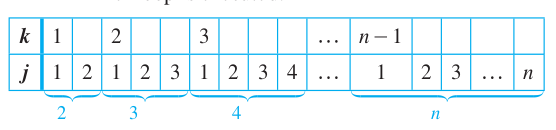
\includegraphics[scale=0.5]{../images/11.3.11.a.png}
\end{figure}

Hence the total number of iterations of the inner loop is \(2+3+\cdots+n = (1+2+3+\cdots+n) - 1 = \frac{n(n+1)}{2} - 1 = 
\frac{1}{2}n^2 + \frac{1}{2}n - 1\) (by Theorem 5.2.1). Because one operation is performed for each iteration of the 
inner loop, the total number of operations is \(\frac{1}{2}n^2 + \frac{1}{2}n - 1\).
\end{proof}

\subsubsection{(b)}
\begin{proof}
By the theorem on polynomial orders, \(\frac{1}{2}n^2 + \frac{1}{2}n - 1\) is \(\Theta(n^2)\), and so the algorithm 
segment has order \(n^2\).
\end{proof}

\subsection{Exercise 12}
\begin{tabbing}
{\bf for} \= \(k \coloneqq 1\) {\bf to} \(n-1\) \\
          \> \(max \coloneqq a[k]\) \\
          \> {\bf for} \= \(i \coloneqq k+1\) {\bf to} \(n\)\\
          \>           \> {\bf if} \(max < a[i]\) {\bf then} \(max \coloneqq a[i]\) \\
          \> {\bf next} \(i\) \\
\(a[k] \coloneqq max\) \\
{\bf next} \(k\)
\end{tabbing}

\subsubsection{(a)}
\begin{proof}
There is 1 comparison operation in the inner loop. The outer loop iterates \(n-1-1+1 = n-1\) times. But the inner loop
iterates a variable number of times. When \(k=1\) the inner loop iterates \(n-2+1 = n-1\) times, when \(k=2\) the inner 
loop iterates \(n-3+1 = n-2\) times, and so on. Finally when \(k=n-1\) the inner loop iterates \(n-(n-1+1)+1 = 1\) times.
The total number of iterations of the inner loop is \((n-1) + (n-2) + \cdots + 2 + 1 = (1+2+ \cdots + n) - n = 
\frac{n(n+1)}{2} - n = \frac{1}{2}n^2 - \frac{1}{2}n\), which is also the total number of operations.
\end{proof}

\subsubsection{(b)}
\begin{proof}
\(\frac{1}{2}n^2 - \frac{1}{2}n\) is \(\Theta(n^2)\) by theorem on polynomial orders, so the algorithm has order 
\(n^2\).
\end{proof}

\subsection{Exercise 13}
\begin{tabbing}
{\bf for} \= \(i \coloneqq 1\) {\bf to} \(n-1\) \\
          \> {\bf for} \= \(j \coloneqq i\) {\bf to} \(n\)\\
          \>           \> {\bf if} \= \(a[j] > a[i]\) {\bf then do} \\
          \>           \>          \>\(temp \coloneqq a[i]\)\\
          \>           \>          \>\(a[i] \coloneqq a[j]\)\\
          \>           \>          \>\(a[j] \coloneqq temp\)\\
          \>           \> {\bf end do} \\
          \> {\bf next} \(j\) \\
{\bf next} \(i\)
\end{tabbing}

\subsubsection{(a)}
\begin{proof}
The inner loop contains 1 comparison operation. When \(i = 1\) the inner loop iterates \(n-1+1 = n\) times, when \(i = 2\) 
the inner loop iterates \(n-2+1 = n-1\) times, and so on. Finally when \(i = n-1\) the inner loop iterates \(n-(n-1)+1\)
= 2 times. The total number of operations is then \(n+(n-1)+ \cdots + 3 + 2 = (1+2+3+ \cdots + n)-1 = \frac{n(n+1)}{2}-1\)
= \(\frac{1}{2}n^2 + \frac{1}{2}n - 1\).
\end{proof}

\subsubsection{(b)}
\begin{proof}
\(\frac{1}{2}n^2 + \frac{1}{2}n - 1\) is \(\Theta(n^2)\) by theorem on polynomial orders, so the algorithm has order 
\(n^2\).
\end{proof}

\subsection{Exercise 14}
\begin{tabbing}
\(t \coloneqq 0\) \\
{\bf for} \= \(i \coloneqq 1\) {\bf to} \(n\) \\
          \> \(s \coloneqq 0\) \\ 
          \> {\bf for} \= \(j \coloneqq 1\) {\bf to} \(i\)\\
          \>           \> \(s \coloneqq s + a[j]\) \\
          \> {\bf next} \(j\) \\
          \> \(t \coloneqq t + s^2\) \\
{\bf next} \(i\)
\end{tabbing}

\subsubsection{(a)}
\begin{proof}
There is one addition for each iteration of the inner loop, and there is one additional addition and one multiplication 
for each iteration of the outer loop. The number of iterations in the inner loop equals the number of columns in the 
following table, which shows the values of \(i\) and \(j\) for which the inner loop is executed.

\begin{figure}[ht!]
\centering
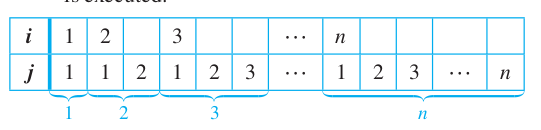
\includegraphics[scale=0.5]{../images/11.3.14.a.png}
\end{figure}

Hence the total number of iterations of the inner loop is = \(1 + 2 + 3 + \cdots + n = \frac{n(n+1)}{2} = \frac{1}{2}n^2 +
\frac{1}{2}n\) (by Theorem 5.2.1). Because one addition is performed for each iteration of the inner loop, the number of 
operations performed when the inner loop is executed is \(\frac{1}{2}n^2 + \frac{1}{2}n\). Now an additional two 
operations are performed each time the outer loop is executed, and because the outer loop is executed \(n\) times, this gives 
an additional \(2n\) operations. Therefore, the total number of operations is \(\frac{1}{2}n^2 + \frac{1}{2}n + 2n\)
= \(\frac{1}{2}n^2 + \frac{5}{2}n\).
\end{proof}

\subsubsection{(b)}
\begin{proof}
By the theorem on polynomial orders, \(\frac{1}{2}n^2 + \frac{5}{2}n\) is \(\Theta(n^2)\), and so the algorithm 
segment has order \(n^2\).
\end{proof}

\subsection{Exercise 15}
\begin{tabbing}
{\bf for} \= \(i \coloneqq 1\) {\bf to} \(n-1\) \\
          \> \(p \coloneqq 1\) \\ 
          \> \(q \coloneqq 1\) \\ 
          \> {\bf for} \= \(j \coloneqq i+1\) {\bf to} \(n\)\\
          \>           \> \(p \coloneqq p \cdot c[j]\) \\
          \>           \> \(q \coloneqq q \cdot c[j]^2\) \\
          \> {\bf next} \(j\) \\
          \> \(r \coloneqq p + q\) \\
{\bf next} \(i\)
\end{tabbing}

\subsubsection{(a)}
\begin{proof}
The inner loop has 3 multiplications, the outer loop has 1 addition.

The inner loop iterates: \(i=1\): \(n-(1+1)+1 = n-1\) times, \(i=2\): \(n-(2+1)+1 = n-2\) times, \(\ldots\), \(i = n-1\):
\(n-(n-1+1)+1 = 1\) time. Total: \(1+2+\cdots+(n-2)+(n-1) = \frac{n(n+1)}{2}-n = \frac{1}{2}n^2 - \frac{1}{2}n\) times.

The outer loop iterates: \(n-1-1+1 = n-1\) times. So the total number of operations is \(3\left(\frac{1}{2}n^2-\frac{1}{2}
n\right) + 1 \cdot (n-1) = \frac{3}{2}n^2 - \frac{1}{2}n -1\).
\end{proof}

\subsubsection{(b)}
\begin{proof}
\(\frac{3}{2}n^2 - \frac{1}{2}n - 1\) is \(\Theta(n^2)\) by theorem on polynomial orders, so the algorithm has order 
\(n^2\).
\end{proof}

\subsection{Exercise 16}
\begin{tabbing}
{\bf for} \= \(i \coloneqq 1\) {\bf to} \(n\) \\
          \> \(s \coloneqq 0\) \\ 
          \> {\bf for} \= \(j \coloneqq 1\) {\bf to} \(i-1\)\\
          \>           \> \(s \coloneqq s + j\cdot (i-j+1)\)\\
          \> {\bf next} \(j\) \\
          \> \(r \coloneqq s^2\) \\
{\bf next} \(i\)
\end{tabbing}

\subsubsection{(a)}
\begin{proof}
The inner loop has 4 operations: 2 additions, 1 subtraction, 1 multiplication. The outer loop has 1 multiplication. The outer
loop iterates \(n-1=1 = n\) times.

When \(i = 1\), the inner loop runs from \(j = 1\) to \(j = i-1 = 1-1 = 0\), so it cannot run (from 1 to 0). I think this
might be a typo in the book.

When \(i = 2\), the inner loop runs from \(j = 1\) to \(j = i-1 = 2-1 = 1\), so it iterates \(1 - 1 + 1 = 1\) time.

When \(i = 3\), the inner loop runs from \(j = 1\) to \(j = i-1 = 3-1 = 2\), so it iterates \(2-1+1=2\) times. And so on.

Finally, when \(i = n\) the inner loop iterates \(n-1 - 1 + 1 = n-1\) times. So the total number of iterations of the inner
loop is \(1+2+\cdots+(n-2)+(n-1) = \frac{(n-1)(n-1+1)}{2} = \frac{1}{2}n^2 - \frac{1}{2}n\).

The total number of operations is: 4 times the inner loop, plus 1 times the outer loop, = \(4\left(\frac{1}{2}n^2-
\frac{1}{2}n\right) + 1 \cdot n = 2n^2 - 2n + n = 2n^2 - n\).
\end{proof}

\subsubsection{(b)}
\begin{proof}
\(2n^2 - n\) is \(\Theta(n^2)\) by theorem on polynomial orders, so the algorithm has order \(n^2\).
\end{proof}

\subsection{Exercise 17}
\begin{tabbing}
{\bf for} \= \(i \coloneqq 1\) {\bf to} \(n\) \\
          \> {\bf for} \= \(j \coloneqq 1\) {\bf to} \(\floor{(i+1)/2}\)\\
          \>           \> \(a \coloneqq (n-i)\cdot(n-j)\) \\
          \> {\bf next} \(j\) \\
{\bf next} \(i\)
\end{tabbing}

\subsubsection{(a)}
\begin{proof}
There are two subtractions and one multiplication for each iteration of the inner loop. If \(n\) is odd, the number of 
iterations of the inner loop equals the number of columns in the following table, which shows the values of \(i\) and \(j\) 
for which the inner loop is executed.

\begin{figure}[ht!]
\centering
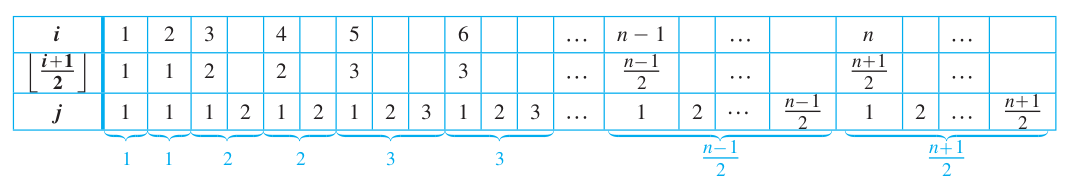
\includegraphics[scale=0.45]{../images/11.3.17.a.png}
\end{figure}

Thus the number of iterations of the inner loop is

\begin{tabular}{rll}
= & \(\dps 1+1+2+2+\cdots+\frac{n-1}{2}+\frac{n-1}{2}+\frac{n+1}{2}\) & {\cy }\\
= & \(\dps 2\left(1+2+3+\cdots+\frac{n-1}{2}\right)+\frac{n+1}{2}\) & {\cy }\\
= & \(\dps 2 \cdot \frac{\frac{n-1}{2}\left(\frac{n-1}{2}+1\right)}{2} + \frac{n+1}{2}\) & {\cy by Theorem 5.2.1}\\
= & \(\dps \frac{n^2-2n+1}{4} + \frac{n-1}{2} + \frac{n+1}{2}\) & {\cy }\\
= & \(\dps \frac{1}{4}n^2+\frac{1}{2}n+\frac{1}{4}\) & {\cy }
\end{tabular}

By similar reasoning, if \(n\) is even, then the number of iterations of the inner loop is

\begin{tabular}{rll}
= & \(\dps 1+1+2+2+\cdots+\frac{n}{2}+\frac{n}{2}\) & {\cy }\\
= & \(\dps 2\left(1+2+3+\cdots+\frac{n}{2}\right)\) & {\cy }\\
= & \(\dps 2 \cdot \frac{\frac{n}{2}\left(\frac{n}{2} + 1 \right)}{2}\) & {\cy by Theorem 5.2.1}\\
= & \(\dps \frac{1}{4}n^2+\frac{1}{2}n\) & {\cy }
\end{tabular}

Because three operations are performed for each iteration of the inner loop, the answer is \(\dps 3 \left(\frac{1}{4}n^2+
\frac{1}{2}n\right)\) when \(n\) is even, and \(\dps 3 \left(\frac{1}{4}n^2+\frac{1}{2}n+\frac{1}{4}\right)\) when 
\(n\) is odd.
\end{proof}

\subsubsection{(b)}
\begin{proof}
Both \(\dps 3 \left(\frac{1}{4}n^2+\frac{1}{2}n\right)\) and \(\dps 3 \left(\frac{1}{4}n^2+\frac{1}{2}n+\frac{1}{4}\right)\) 
are \(\Theta(n^2)\) by theorem on polynomial orders, so the algorithm has order \(n^2\).
\end{proof}

\subsection{Exercise 18}
\begin{tabbing}
{\bf for} \= \(i \coloneqq 1\) {\bf to} \(n\) \\
          \> {\bf for} \= \(j \coloneqq \floor{(i+1)/2}\) {\bf to} \(n\) \\
          \>           \> \(x \coloneqq i \cdot j\) \\
          \> {\bf next} \(j\) \\
{\bf next} \(i\)
\end{tabbing}

\subsubsection{(a)}
\begin{proof}
When \(i=1\) the inner loop runs from \(j = \floor{(1+1)/2} = 1\) to \(n\), so it iterates \(n-1+1 = n\) times.

When \(i=2\) the inner loop runs from \(j = \floor{(2+1)/2} = 1\) to \(n\), so it iterates \(n-1+1 = n\) times.

When \(i=3\) the inner loop runs from \(j = \floor{(3+1)/2} = 2\) to \(n\), so it iterates \(n-2+1 = n-1\) times.

When \(i=4\) the inner loop runs from \(j = \floor{(4+1)/2} = 2\) to \(n\), so it iterates \(n-2+1 = n-1\) times.

And so on. Finally when \(i = n\) the inner loop runs from \(j = \floor{(n+1)/2}\) to \(n\). If \(n\) is even, this is from
\(n/2\) to \(n\); and if \(n\) is odd this is from \((n+1)/2\) to \(n\). So it iterates roughly \(n/2\) times.

So the total iterations of the inner loop is \(n+n+(n-1)+(n-1)+ \cdots + (n/2 + n/2) = 2(\frac{n}{2} + \cdots + (n-1) + n)\)
\(= 2(1+2+ \cdots + n - (1+2+ \cdots \frac{n}{2})) = 2 \left( \frac{n(n+1)}{2}-\frac{\frac{n}{2}(\frac{n}{2}+1)}{2}\right)\)
\(= n(n+1) - \frac{n}{2}(\frac{n}{2}+1) = n^2 + n - \frac{1}{4}n^2 - \frac{1}{2}n = \frac{3}{4}n^2 - \frac{1}{2}n\).

This is the same as the number of operations, as there is only one multiplication inside the inner loop. 
\end{proof}

\subsubsection{(b)}
\begin{proof}
\(\frac{3}{4}n^2 - \frac{1}{2}n\) is \(\Theta(n^2)\) by theorem on polynomial orders. So the algorithm has order 
\(n^2\).
\end{proof}

\subsection{Exercise 19}
\begin{tabbing}
{\bf for} \= \(i \coloneqq 1\) {\bf to} \(n\) \\
          \> {\bf for} \= \(j \coloneqq 1\) {\bf to} \(i\) \\
          \>           \> {\bf for} \= \(k \coloneqq 1\) {\bf to} \(j\) \\
          \>           \>           \> \(x \coloneqq i \cdot j \cdot k\) \\
          \>           \> {\bf next} \(k\) \\
          \> {\bf next} \(j\) \\
{\bf next} \(i\)
\end{tabbing}

{\it Hint:} See Section 9.6 for a discussion of how to count the number of iterations of the innermost loop.

\subsubsection{(a)}
\begin{proof}
By Example 9.6.4 there are \([n(n + 1)(n + 2)]/6\) iterations of the innermost loop. There are two multiplications, so the
total number of operations is \([n(n + 1)(n + 2)]/3 = \frac{1}{3}(n^3 + 3n^2 + 2n)\).
\end{proof}

\subsubsection{(b)}
\begin{proof}
\(\frac{1}{3}(n^3 + 3n^2 + 2n)\) is \(\Theta(n^3)\) by theorem on polynomial orders. So the algorithm has order \(n^3\).
\end{proof}

\subsection{Exercise 20}
Construct a table showing the result of each step when insertion sort is applied to the array \(a[1] = 6\), 
\(a[2] = 2, a[3] = 1, a[4] = 8\), and \(a[5] = 4\).

\begin{proof}
\begin{center}
\arrayrulecolor{cyan}
\begin{tabular}{|c|c|c|c|c|c|}
\hline
& \(a[1]\) & \(a[2]\) & \(a[3]\) & \(a[4]\) & \(a[5]\) \\
\hline
{\bf Initial order} &6&2&1&8&4 \\
\hline
{\bf Step 1 result} &2&6&1&8&4 \\
\hline
{\bf Step 2 result} &1&2&6&8&4 \\
\hline
{\bf Step 3 result} &1&2&6&8&4 \\
\hline
{\bf Final order} &1&2&4&6&8 \\
\hline
\end{tabular}
\arrayrulecolor{black} % change it back!
\end{center}
\end{proof}

\subsection{Exercise 21}
Construct a table showing the result of each step when insertion sort is applied to the array \(a[1] = 7\), 
\(a[2] = 3, a[3] = 6, a[4] = 9\), and \(a[5] = 5\).

\begin{proof}
\begin{center}
\arrayrulecolor{cyan}
\begin{tabular}{|c|c|c|c|c|c|}
\hline
& \(a[1]\) & \(a[2]\) & \(a[3]\) & \(a[4]\) & \(a[5]\) \\
\hline
{\bf Initial order} &7&3&6&9&5 \\
\hline
{\bf Step 1 result} &3&7&6&9&5 \\
\hline
{\bf Step 2 result} &3&6&7&9&5 \\
\hline
{\bf Step 3 result} &3&6&7&9&5 \\
\hline
{\bf Final order} &3&5&6&7&9 \\
\hline
\end{tabular}
\arrayrulecolor{black} % change it back!
\end{center}
\end{proof}

\subsection{Exercise 22}
Construct a trace table showing the action of insertion sort on the array of exercise 20.

\begin{proof}
\begin{center}
\arrayrulecolor{cyan}
\begin{tabular}{|c|c|c|c|c|c|c|c|c|c|c|c|}
\hline
\(\bm{n}\) &5&&&&&&&&&& \\
\hline
\(\bm{a[1]}\) &6&2&&&1&&&&&& \\
\hline
\(\bm{a[2]}\) &2&6&&1&2&&&&&& \\
\hline
\(\bm{a[3]}\) &1&&&6&&&&&&4& \\
\hline
\(\bm{a[4]}\) &8&&&&&&&&4&6& \\
\hline
\(\bm{a[5]}\) &4&&&&&&&&8&& \\
\hline
\(\bm{k}\) &2&&3&&&4&&5&&& \\
\hline
\(\bm{x}\) &2&&1&&&8&&4&&& \\
\hline
\(\bm{j}\) &1&0&2&1&0&3&0&4&3&2&0 \\
\hline
\end{tabular}
\arrayrulecolor{black} % change it back!
\end{center}
\end{proof}

\subsection{Exercise 23}
Construct a trace table showing the action of insertion sort on the array of exercise 21.

\begin{proof}
\begin{center}
\arrayrulecolor{cyan}
\begin{tabular}{|c|c|c|c|c|c|c|c|c|c|c|c|c|}
\hline
\(\bm{n}\) &5&&&&&&&&&&& \\
\hline
\(\bm{a[1]}\) &7&3&&&&&&&&&& \\
\hline
\(\bm{a[2]}\) &3&7&&6&&&&&&&5& \\
\hline
\(\bm{a[3]}\) &6&&&7&&&&&&5&6& \\
\hline
\(\bm{a[4]}\) &9&&&&&&&&5&7&& \\
\hline
\(\bm{a[5]}\) &5&&&&&&&&9&&& \\
\hline
\(\bm{k}\) &2&&3&&&4&&5&&&& \\
\hline
\(\bm{x}\) &3&&6&&&9&&5&&&& \\
\hline
\(\bm{j}\) &1&0&2&1&0&3&0&4&3&2&1&0 \\
\hline
\end{tabular}
\arrayrulecolor{black} % change it back!
\end{center}
\end{proof}

\subsection{Exercise 24}
How many comparisons between values of \(a[j]\) and \(x\) actually occur when insertion sort is applied to the array of 
exercise 20?

\begin{proof}
There are seven comparisons between values of \(x\) and values of \(a[j]\): one when \(k = 2\), two when \(k = 3\), one when 
\(k = 4\), and three when \(k = 5\).
\end{proof}

\subsection{Exercise 25}
How many comparisons between values of \(a[j]\) and \(x\) actually occur when insertion sort is applied to the array of 
exercise 21?

\begin{proof}
There are eight comparisons between values of \(x\) and values of \(a[j]\): one when \(k = 2\), two when \(k = 3\), one when 
\(k = 4\), and four when \(k = 5\).
\end{proof}

\subsection{Exercise 26}
According to Example 11.3.6, the maximum number of comparisons needed to perform insertion sort on an array of length five is 
\(\frac{1}{2}(5^2 + 5 - 2) = 14\). Find an array of length five that requires the maximum number of comparisons when 
insertion sort is applied to it.

\begin{proof}
Example 11.3.6 has a mistake. It says that the maximum number of comparisons for any \(k\) is \(k-1\), then it says that 
\(k\) goes from 2 to \(n\), so the sum should be: \((2-1) + (3-1) + \cdots + (n-1-1) + (n-1) = 1+2+\cdots+(n-2)+(n-1)\),
which is equal to \(\dps\frac{(n-1)(n-1+1)}{2} = \frac{1}{2}n^2 - \frac{1}{2}n\).

Let \(a = [5,4,3,2,1]\). When \(k=2\) 4 will be compared to 5 and swapped. When \(k=3\), 3 will be compared to 5 first, and
swapped with it, then it will be compared to 4 and swapped with it. Similarly there will be 3 comparisons when \(k=4\)
and finally 4 comparisons when \(k=5\), for a total of \(1+2+3+4 = 10\). This matches the formula above, since 
\(\dps\frac{1}{2}5^2 - \frac{1}{2}5 = 25/2 - 5/2 = 20/2= 10\).
\end{proof}

\subsection{Exercise 27}
Consider the recurrence relation that arose in Example 11.3.7: \(E_1 = 0\) and \(E_k = E_{k-1} + \frac{k+1}{2}\), for each 
integer \(k \geq 2\).

\subsubsection{(a)}
Use iteration to find an explicit formula for the sequence.

{\it Hint:} \(E_n = \frac{1}{2}[3 + 4 + \cdots + (n + 1)]\), which equals \(\frac{1}{2}[(1 + 2 + 3 + \cdots + (n + 1)) - 
(1 + 2)]\).

\begin{proof}
\(E_1 = 0\), \(E_2 = E_1 + \frac{2+1}{2} = 3/2\), \(E_3 = E_2 + \frac{3+1}{2} = 3/2+4/2 = (3+4)/2\), \\
\(E_4 = E_3 + \frac{4+1}{2} = (3+4)/2 + 5/2 = (3+4+5)/2\), \\
\(E_5 = E_4 + \frac{5+1}{2} = (3+4+5)/2 + 6/2 = (3+4+5+6)/2\).

We guess \(E_n = (3+4+\cdots+n)/2\).
\end{proof}

\subsubsection{(b)}
Use mathematical induction to verify the correctness of the formula.

\begin{proof}
Let \(P(n)\) be the equation \(E_n = (3+4+\cdots+n)/2\).

{\bf Show that \(P(2)\) is true:} \(E_2 = 3/2\) which agrees with the formula above, so \(P(2)\) is true.

{\bf Show that for any integer \(k \geq 2\) if \(P(k)\) is true then \(P(k+1)\) is true:} Assume \(k \geq 2\) is any 
integer and \(E_k = (3+4+\cdots+k)/2\). {\it [We want to show \(E_{k+1} = (3+4+\cdots+k+(k+1))/2\).]}

\(E_{k+1} = E_k + \frac{k+1}{2} = (3+4+\cdots+k)/2 + \frac{k+1}{2} = (3+4+\cdots+k+(k+1))/2\), so \(P(k+1)\) holds.
\end{proof}

{\bf \cy Exercises \(28-35\) refer to selection sort, which is another algorithm to arrange the items in an array in 
ascending order.}

\begin{tcolorbox}[colframe=cyan]
{\bf \cy Algorithm 11.3.2 Selection Sort}

{\it [Given an array \(a[1], a[2], a[3], \ldots, a[n]\), this algorithm selects the smallest element and places it in the 
first position, then selects the second smallest element and places it in the second position, and so forth, until the 
entire array is sorted. In general, for each \(k = 1\) to \(n - 1\), the \(k\)th step of the algorithm selects the index of 
the array item with minimum value from among \(a[k + 1], a[k + 2], a[k + 3], \ldots, a[n]\). Once this index is found, the 
value of the corresponding array item is interchanged with the value of \(a[k]\) unless the index already equals \(k\). At 
the end of execution the array elements are in order.]}

{\bf Input:} \(n\) {\it [a positive integer]}, \(a[1], a[2], a[3], \ldots, a[n]\) {\it [an array of data items capable of 
being ordered]}

{\bf Algorithm Body:} 
\begin{tabbing}
{\bf for} \= \(k \coloneqq 1\) {\bf to} \(n-1\) \\
          \> \(indexMin \coloneqq k\) \\
          \> {\bf for} \= \(i \coloneqq k+1\) {\bf to} \(n\)\\
          \>           \> {\bf if} \(a[i] < a[indexMin]\) \\
          \>           \> {\bf then} \(indexMin\coloneqq i\)\\
          \> {\bf next} \(i\) \\
          \> {\bf if} \(indexMin \neq k\) {\bf then} \\
          \>           \> \(Temp \coloneqq a[k]\) \\
          \>           \> \(a[k] \coloneqq a[indexMin]\) \\
          \>           \> \(a[indexMin] \coloneqq Temp\) \\
{\bf next} \(k\)
\end{tabbing}

{\bf Output:} \(a[1], a[2], a[3], \ldots, a[n]\) {\it [in ascending order]}

The action of selection sort can be represented pictorially as follows:

\begin{tabular}{ccccccc}
\(a[1]\) & \(a[2]\) & \(\cdots\) & \(\boxed{a[k]}\) & \(a[k+1]\) & \(\cdots\) & \(a[n]\) \\
&&&{\cy \(\ua\)}&&&
\end{tabular}

{\cy \(k\)th step: Find the index of the array element with minimum value from among \(a[k + 1], \ldots, a[n]\). If the 
value of this array element is less than the value of \(a[k]\), then its value and the value of \(a[k]\) are 
interchanged.}
\end{tcolorbox}

\subsection{Exercise 28}
Construct a table showing the interchanges that occur when selection sort is applied to the array \(a[1] = 7, a[2] = 3\), 
\(a[3] = 8, a[4] = 4\), and \(a[5] = 2\).

\begin{proof}
The top row of the table shows the initial values of the array, and the bottom row shows the final values. The results 
for executing each step in the for-next loop are shown in separate rows.

\begin{figure}[ht!]
\centering
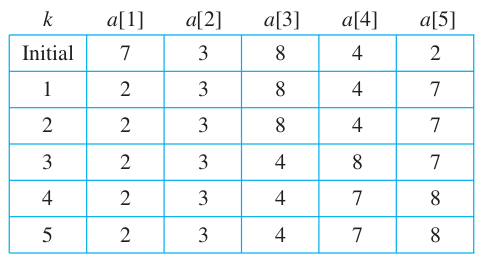
\includegraphics[scale=0.6]{../images/11.3.28.png}
\end{figure}
\end{proof}

\subsection{Exercise 29}
Construct a table showing the interchanges that occur when selection sort is applied to the array \(a[1] = 6, a[2] = 4\), 
\(a[3] = 5, a[4] = 8\), and \(a[5] = 1\).

\begin{proof}
\begin{center}
\arrayrulecolor{cyan}
\begin{tabular}{|c|c|c|c|c|c|}
\hline
\(k\)& \(a[1]\) & \(a[2]\) & \(a[3]\) & \(a[4]\) & \(a[5]\) \\
\hline
Initial&6&4&5&8&1 \\
\hline
1&1&4&5&8&6 \\
\hline
2&1&4&5&8&6 \\
\hline
3&1&4&5&8&6 \\
\hline
4&1&4&5&6&8\\
\hline
Final&1&4&5&6&8\\
\hline
\end{tabular}
\arrayrulecolor{black} % change it back!
\end{center}
\end{proof}

\subsection{Exercise 30}
Construct a trace table showing the action of selection sort on the array of exercise 28.

\begin{proof}
\begin{figure}[ht!]
\centering
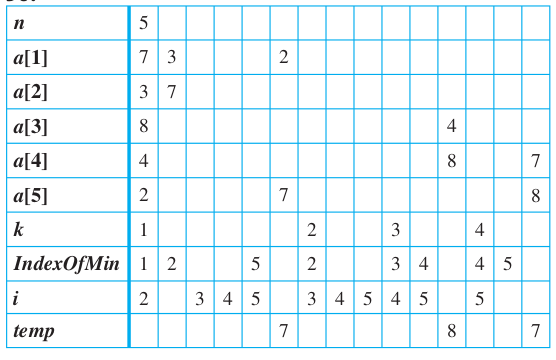
\includegraphics[scale=0.6]{../images/11.3.30.png}
\end{figure}
\end{proof}

\subsection{Exercise 31}
Construct a trace table showing the action of selection sort on the array of exercise 29.

\begin{proof}
\begin{center}
\arrayrulecolor{cyan}
\begin{tabular}{|c|c|c|c|c|c|c|c|c|c|c|c|c|c|c|}
\hline
\(\bm{n}\)        &5& & & & & & & & & & & & & \\
\hline
\(\bm{a[1]}\)     &6& & & & &1& & & & & & & & \\
\hline
\(\bm{a[2]}\)     &4& & & & & & & & & & & & & \\
\hline
\(\bm{a[3]}\)     &5& & & & & & & & & & & & & \\
\hline
\(\bm{a[4]}\)     &8& & & & & & & & & & & & &6 \\
\hline
\(\bm{a[5]}\)     &1& & & & &6& & & & & & & &8 \\
\hline
\(\bm{k}\)        &1& & & & & &2& & &3& &4& & \\
\hline
\(\bm{indexMin}\) &1&2& & &5& &2& & &3& &4&5& \\
\hline
\(\bm{i}\)        &2& &3&4&5& &3&4&5&4&5&5& & \\
\hline
\(\bm{temp}\)     & & & & & &6& & & & & & & &8 \\
\hline
\end{tabular}
\arrayrulecolor{black} % change it back!
\end{center}
\end{proof}

\subsection{Exercise 32}
When selection sort is applied to the array of exercise 28, how many times is the comparison in the if-then statement 
performed?

{\it Note:} The book is not clear about this, but it is referring to the if-then comparison inside the inner for-loop,
not to the ``{\bf if \(IndexOfMin \neq k\) then}'' after it.

\begin{proof}
There is one comparison for each combination of values of \(k\) and \(i\): namely, \(4 + 3 + 2 + 1 = 10\).
\end{proof}

\subsection{Exercise 33}
When selection sort is applied to the array of exercise 29, how many times is the comparison in the if-then statement 
performed?

\begin{proof}
There is one comparison for each combination of values of \(k\) and \(i\): namely, \(4 + 3 + 2 + 1 = 10\).
\end{proof}

\subsection{Exercise 34}
When selection sort is applied to an array \(a[1], a[2], a[3], a[4]\), how many times is the comparison in the if-then 
statement performed?

\begin{proof}
\(k\) ranges from 1 to \(4-1=3\), and for each value of \(k\), \(i\) ranges from \(k+1\) to \(4\). So \(i\) ranges from: 
2 to 4, then 3 to 4, then 4 to 4. So \((4-2+1) + (4-3+1) + (4-4+1) = 3+2+1 = 6\) comparisons.
\end{proof}

\subsection{Exercise 35}
Consider applying selection sort to an array \(a[1], a[2], a[3], \ldots, a[n]\).

\subsubsection{(a)}
How many times is the comparison in the {\bf if-then} statement performed when \(a[1]\) is compared to each of 
\(a[2], a[3], \ldots, a[n]\)?

\begin{proof}
Since \(k = 1\), \(i\) ranges from \(k=2\) to \(n\), so \(n-2+1 = n-1\) times.
\end{proof}

\subsubsection{(b)}
How many times is the comparison in the {\bf if-then} statement performed when \(a[2]\) is compared to each of 
\(a[3], a[4], \ldots, a[n]\)?

\begin{proof}
Since \(k = 2\), \(i\) ranges from \(k=3\) to \(n\), so \(n-3+1 = n-2\) times.
\end{proof}

\subsubsection{(c)}
How many times is the comparison in the {\bf if-then} statement performed when \(a[k]\) is compared to each of 
\(a[k+1], a[k+2], \ldots, a[n]\)?

\begin{proof}
\(i\) ranges from \(k+1\) to \(n\), so \(n-(k+1)+1 = n-k\) times.
\end{proof}

\subsubsection{(d)}
Using the number of times the comparison in the if-then statement is performed as a measure of the time efficiency of 
selection sort, find a worst-case order for selection sort. Use the theorem on polynomial orders.

{\it Hint:} The answer is \(n^2\).

\begin{proof}
From parts (a), (b), (c) the total number of comparisons is: \((n-1) + (n-2) + \cdots + (n-(n-1)) = 1+2+\cdots+(n-1) =
\frac{(n-1)(n-1+1)}{2} = \frac{1}{2}n^2 - \frac{1}{2}n\). This is \(\Theta(n^2)\) by theorem on polynomial orders, so the 
algorithm has order \(n^2\).
\end{proof}

{\bf \cy Exercises \(36-39\) refer to the following algorithm to compute the value of a real polynomial.}

\begin{tcolorbox}[colframe=cyan]
{\bf \cy Algorithm 11.3.3 Term-by-Term Polynomial Evaluation}

{\it [This algorithm computes the value of a polynomial \(a[n]x^n + a[n-1]x^{n-1} + \cdots + a[2]x^2 + a[1]x + a[0]\) 
by computing each term separately, starting with \(a[0]\), and adding it to an accumulating sum.]}

{\bf Input:} \(n\) {\it [a nonnegative integer]}, \(a[0], a[1], a[2], a[3], \ldots, a[n]\) {\it [an array of real 
numbers]}, \(x\) {\it [a real number]}

{\bf Algorithm Body:} 
\begin{tabbing}
\(polyval \coloneqq a[0]\) \\
{\bf for} \= \(i \coloneqq 1\) {\bf to} \(n\) \\
          \> \(term \coloneqq a[i]\) \\
          \> {\bf for} \= \(j \coloneqq 1\) {\bf to} \(i\)\\
          \>           \> \(term \coloneqq term \cdot x\)\\
          \> {\bf next} \(j\) \\
          \> \(polyval \coloneqq polyval + term\) \\
{\bf next} \(i\)
\end{tabbing}

{\it [At this point \(polyval = a[n]x^n + a[n-1]x^{n-1} + \cdots + a[2]x^2 + a[1]^x + a[0]\).]}

{\bf Output:} \(polyval\) {\it [a real number]}
\end{tcolorbox}

\subsection{Exercise 36}
Trace Algorithm 11.3.3 for the input \(n = 3, a[0] = 2, a[1] = 1, a[2] = -1, a[3] = 3\), and \(x = 2\).

\begin{proof}
\begin{figure}[ht!]
\centering
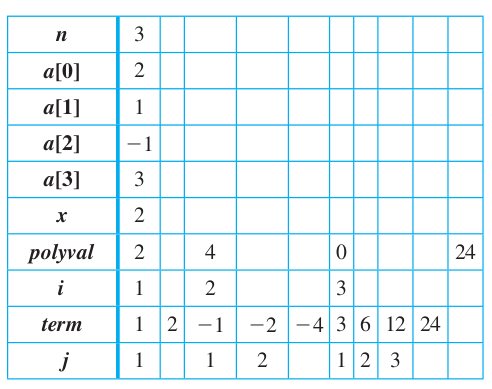
\includegraphics[scale=0.6]{../images/11.3.36.png}
\end{figure}
\end{proof}

\subsection{Exercise 37}
Trace Algorithm 11.3.3 for the input \(n = 2, a[0] = 5, a[1] = -1, a[2] = 2\), and \(x = 3\).

\begin{proof}
\begin{center}
\arrayrulecolor{cyan}
\begin{tabular}{|c|c|c|c|c|c|c|c|}
\hline
\(\bm{n}\)       &2&    & & &  &  \\
\hline
\(\bm{a[0]}\)    &5&    & & &  &  \\
\hline
\(\bm{a[1]}\) &$-1$&    & & &  &  \\
\hline
\(\bm{a[2]}\)    &2&    & & &  &  \\
\hline
\(\bm{x}\)       &3&    & & &  &  \\
\hline
\(\bm{polyval}\) &5&    &2& &  &20\\
\hline
\(\bm{i}\)       &1&    &2& &  &  \\
\hline
\(\bm{term}\) &$-1$&$-3$&2&6&18&  \\
\hline
\(\bm{j}\)       &1&    &1&2&  &  \\
\hline
\end{tabular}
\arrayrulecolor{black} % change it back!
\end{center}
\end{proof}

\subsection{Exercise 38}
Let \(s_n =\) the number of additions and multiplications that are performed when Algorithm 11.3.3 is executed for a 
polynomial of degree \(n\). Express \(s_n\) as a function of \(n\).

\begin{proof}
Number of multiplications = number of iterations of the inner loop = \(1 +2+ 3 + \cdots + n = n(n + 1)/2\) by Theorem 5.2.1.
Number of additions = number of iterations of the outer loop = \(n\). Hence the total number of multiplications and additions 
is \(n(n + 1)/2 + n = n^2/2 + 3n/2\).
\end{proof}

\subsection{Exercise 39}
Use the theorem on polynomial orders to find an order for Algorithm 11.3.3.

\begin{proof}
It's \(n^2\).
\end{proof}

{\bf \cy Exercises \(40-42\) refer to another algorithm, known as Horner’s rule, for finding the value of a polynomial.}

\begin{tcolorbox}[colframe=cyan]
{\bf \cy Algorithm 11.3.4 Horner's Rule}

{\it [This algorithm computes the value of a polynomial \(a[n]x^n + a[n-1]x^{n-1} + \cdots + a[2]x^2 + a[1]x + a[0]\) 
by nesting successive additions and multiplications as indicated in the following parenthesization: \(((\cdots((a[n]x 
+ a[n-1])x + a[n-2])x + \cdots + a[2])x + a[1])x + a[0].\) At each stage, starting with a[n], the current value of polyval 
is multiplied by \(x\) and the next lower coefficient of the polynomial is added to it.]}

{\bf Input:} \(n\) {\it [a nonnegative integer]}, \(a[0], a[1], a[2], a[3], \ldots, a[n]\) {\it [an array of real 
numbers]}, \(x\) {\it [a real number]}

{\bf Algorithm Body:} 
\begin{tabbing}
\(polyval \coloneqq a[n]\) \\
{\bf for} \= \(i \coloneqq 1\) {\bf to} \(n\) \\
          \> \(polyval \coloneqq polyval \cdot x + a[n-i]\) \\
{\bf next} \(i\)
\end{tabbing}

{\it [At this point \(polyval = a[n]x^n + a[n-1]x^{n-1} + \cdots + a[2]x^2 + a[1]^x + a[0]\).]}

{\bf Output:} \(polyval\) {\it [a real number]}
\end{tcolorbox}

\subsection{Exercise 40}
Trace Algorithm 11.3.4 for the input \(n = 3, a[0] = 2, a[1] = 1, a[2] = -1, a[3] = 3\), and \(x = 2\).

\begin{proof}
\begin{figure}[ht!]
\centering
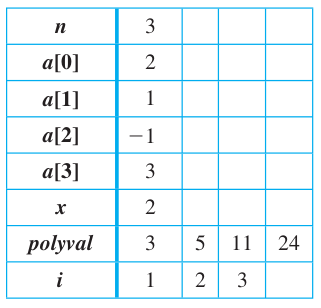
\includegraphics[scale=0.6]{../images/11.3.40.png}
\end{figure}
\end{proof}

\subsection{Exercise 41}
Trace Algorithm 11.3.4 for the input \(n = 2, a[0] = 5, a[1] = -1, a[2] = 2\), and \(x = 3\).

\begin{proof}
\begin{center}
\arrayrulecolor{cyan}
\begin{tabular}{|c|c|c|c|}
\hline
\(\bm{n}\)       &2&  &   \\
\hline
\(\bm{a[0]}\)    &5&  &   \\
\hline
\(\bm{a[1]}\) &$-1$&  &   \\
\hline
\(\bm{a[2]}\)    &2&  &   \\
\hline
\(\bm{x}\)       &3&  &   \\
\hline
\(\bm{polyval}\) &2& 5&20 \\
\hline
\(\bm{i}\)       &1& 2&   \\
\hline
\end{tabular}
\arrayrulecolor{black} % change it back!
\end{center}
\end{proof}

\subsection{Exercise 42}
Let \(t_n =\) the number of additions and multiplications that are performed when Algorithm 11.3.4 is executed for a 
polynomial of degree \(n\). Express \(t_n\) as a function of \(n\).

{\it Hint:} \(t_n = 2n\).

\begin{proof}
There is one multiplication and one subtraction for each iteration of the loop. The loop iterates \(n\) times. 
Therefore \(t_n = 2n\).
\end{proof}

\subsection{Exercise 43}
Use the theorem on polynomial orders to find an order for Algorithm 11.3.4. How does this order compare with that of 
Algorithm 11.3.3?

\begin{proof}
The order is \(n\) which is one degree less than the order of Algorithm 11.3.3. So this algorithm runs in the square root of
the time the other one takes to run.
\end{proof}

\section{Exercise Set 11.4}
{\bf \cy Graph each function defined in \(1-8\).}

\subsection{Exercise 1}
\(f(x) = 3^x\) for each real number \(x\)

\begin{proof}
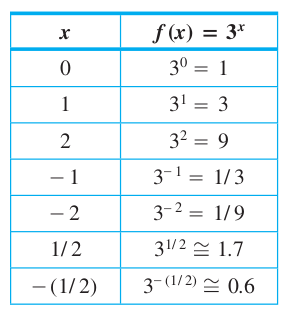
\includegraphics[scale=0.5]{../images/11.4.1.1.png}
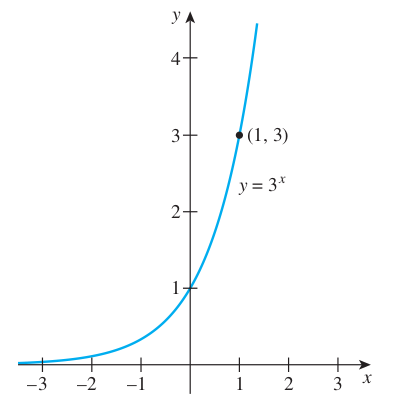
\includegraphics[scale=0.5]{../images/11.4.1.2.png}
\end{proof}

\subsection{Exercise 2}
\(g(x) = \left(\frac{1}{3}\right)^x\) for each real number \(x\)

\begin{proof}
\begin{figure}[ht!]
\centering
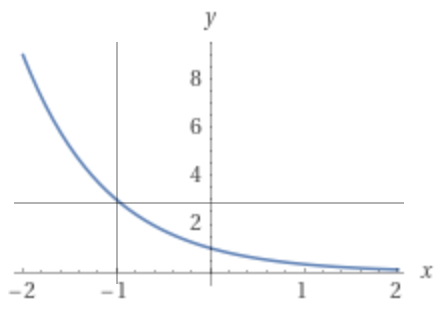
\includegraphics[scale=0.5]{../images/11.4.2.png}
\end{figure}
\end{proof}

\subsection{Exercise 3}
\(h(x) = \log_{10} x\) for each positive real number \(x\)

\begin{proof}
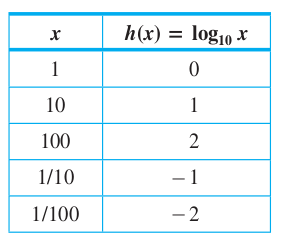
\includegraphics[scale=0.5]{../images/11.4.3.1.png}
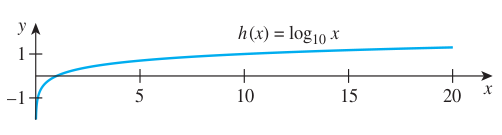
\includegraphics[scale=0.5]{../images/11.4.3.2.png}
\end{proof}

\subsection{Exercise 4}
\(k(x) = \log_2 x\) for each positive real number \(x\)

\begin{proof}
\begin{figure}[ht!]
\centering
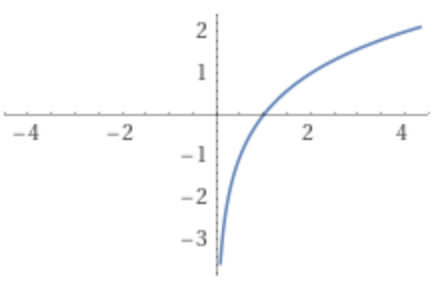
\includegraphics[scale=0.5]{../images/11.4.4.png}
\end{figure}
\end{proof}

\subsection{Exercise 5}
\(F(x) = \floor{\log_2 x}\) for each positive real number \(x\)

\begin{proof}
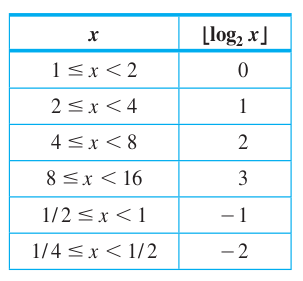
\includegraphics[scale=0.5]{../images/11.4.5.1.png}
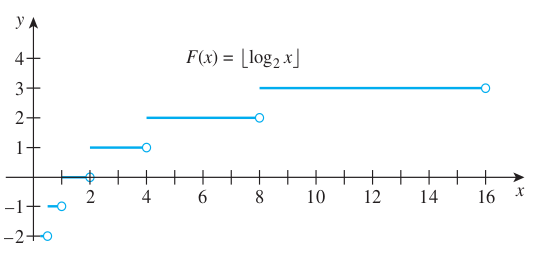
\includegraphics[scale=0.5]{../images/11.4.5.2.png}
\end{proof}

\subsection{Exercise 6}
\(G(x) = \ceil{\log_2 x}\) for each positive real number \(x\)

\begin{proof}
\begin{figure}[ht!]
\centering
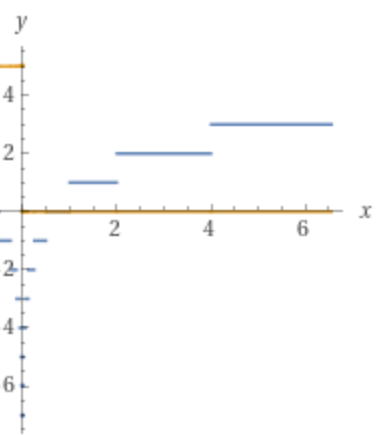
\includegraphics[scale=0.5]{../images/11.4.6.png}
\end{figure}
\end{proof}

\subsection{Exercise 7}
\(H(x) = x \log_2(x)\) for each positive real number \(x\)

\begin{proof}
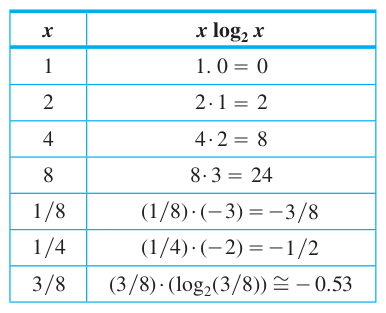
\includegraphics[scale=0.5]{../images/11.4.7.1.png}
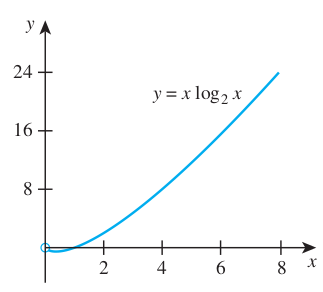
\includegraphics[scale=0.5]{../images/11.4.7.2.png}
\end{proof}

\subsection{Exercise 8}
\(K(x) = x \log_{10} x\) for each positive real number \(x\)

\begin{proof}
\begin{figure}[ht!]
\centering
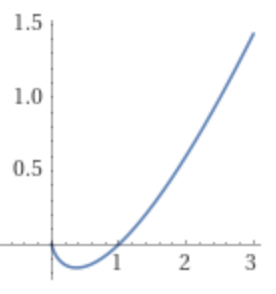
\includegraphics[scale=0.5]{../images/11.4.8.png}
\end{figure}
\end{proof}

\subsection{Exercise 9}
The scale of the graph shown in Figure 11.4.1 is one-fourth inch to each unit. If the point \((2, 2^{64})\) is plotted on 
the graph of \(y = 2^x\), how many miles will it lie above the horizontal axis? What is the ratio of the height of the point 
to the distance of the earth from the sun? (There are 12 inches per foot and 5,280 feet per mile. The earth is 
approximately 93,000,000 miles from the sun on average.) (1/4 inch \(\approx\) 0.635 cm, 1 mile \(\approx\) 0.62 km)

\begin{proof}
The distance above the axis is \(\dps (2^{64} \text{units}) \cdot\left(\frac{1}{4}\frac{\text{inch}}{\text{unit}}\right)\)
= \(\dps \frac{2^{64}}{4}\) inches = \(\dps \frac{2^{64}}{4 \cdot 12 \cdot 5280}\) miles \(\approx 72,785,448,520,000\)
miles. The ratio of the height of the point to the average distance of the earth to the sun is approximately 
72785448520000/93000000 \(\approx\) 782,639. (If you perform the computation using metric units and the approximation 0.635 
cm \(\approx\) 1/4 inch, the ratio comes out to be approximately 780,912.)
\end{proof}

\subsection{Exercise 10}
\subsubsection{(a)}
Use the definition of logarithm to show that \(\log_b(b^x) = x\) for every real number \(x\).

\begin{proof}
By definition of logarithm,  \(\log_b (b^x)\) is the exponent to which \(b\) must be raised to obtain \(b^x\). But, when 
\(b\) is actually raised to the exponent \(x\), \(b^x\) is obtained. That is, \(\log_b (b^x) = x\).
\end{proof}

\subsubsection{(b)}
Use the definition of logarithm to show that \(b\log_b(x) = x\) for every positive real number \(x\).

\begin{proof}
By definition of logarithm,  \(\log_b x\) is the exponent to which \(b\) must be raised to obtain \(x\). Thus when \(b\) is 
actually raised to this exponent, \(x\) is obtained. That is, \(b^{\log_b x} = x\).
\end{proof}

\subsubsection{(c)}
By the result of exercise 28 in Section 7.3, if \(f: X \to Y\) and \(g: Y \to X\) are functions and \(g \circ f = I_X\) and 
\(f \circ g = I_Y\), then \(f\) and \(g\) are inverse functions. Use this result to show that \(\log_b\) and 
\(exp_b\) (the exponential function with base b) are inverse functions.

\begin{proof}
Let \(X = (0, \infty), Y = \R\), let \(f: X \to Y\) be defined by \(f(x) = \log_b(x)\) and let \(g: Y \to X\) be defined by 
\(g(y) = exp_b(y) = b^y\). Then by part (a) \(f(g(y)) = \log_b(b^y) = y\) therefore \(f \circ g = I_Y\). By part (b)
\(g(f(x)) = b^{\log_b(x)} = x\), so \(g \circ f = I_X\). Therefore \(f\) and \(g\) are inverse functions.
\end{proof}

\subsection{Exercise 11}
Let \(b > 1\).

\subsubsection{(a)}
Use the fact that \(u = \log_b(v) \iff v = b^u\) to show that a point \((u, v)\) lies on the graph of the logarithmic 
function with base \(b\) if, and only if, \((v, u)\) lies on the graph of the exponential function with base \(b\).

\begin{proof}
Assume \((u, v)\) lies on the graph of the logarithmic 
function with base \(b\). Then by definition of the 
logarithmic function with base \(b\), \(v = \log_b(u)\). Then \(u = b^v\). Then \((v, u)\) lies on the graph of the 
exponential function with base \(b\). The other direction of the proof follows the same way by reversing the argument.
\end{proof}

\subsubsection{(b)}
Plot several pairs of points of the form \((u, v)\) and \((v, u)\) on a coordinate system. Describe the geometric 
relationship between the locations of the points in each pair.

\begin{proof}
\begin{figure}[ht!]
\centering
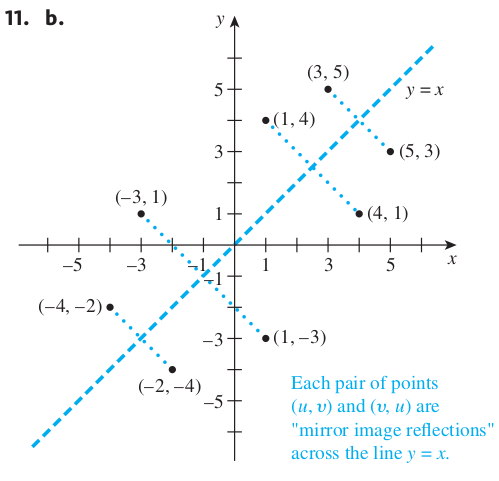
\includegraphics[scale=0.5]{../images/11.4.11.b.png}
\end{figure}
\end{proof}

\subsubsection{(c)}
Draw the graphs of \(y = \log_2 x\) and \(y = 2^x\). Describe the geometric relationship between these graphs.

\begin{proof}
\begin{figure}[ht!]
\centering
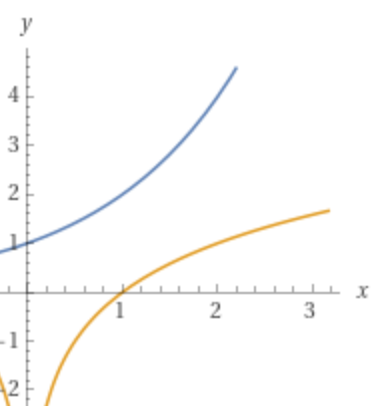
\includegraphics[scale=0.5]{../images/11.4.11.c.png}
\end{figure}

They are symmetric across the diagonal line \(y = x\).
\end{proof}

\subsection{Exercise 12}
Give a graphical interpretation for property (11.4.2) in Example 11.4.1(a) for \(0 < x < 1\).

\begin{proof}
{\it ???}
\end{proof}

\subsection{Exercise 13}
Suppose a positive real number \(x\) satisfies the inequality \(10^m \leq x < 10^{m+1}\) where \(m\) is an integer. What can 
be inferred about \(\floor{\log_{10} x}\)? Justify your answer.

\begin{proof}
\(\floor{\log_{10} x} = m\). This is just like Example 11.4.1 (a) but with base 10 instead. Since \(\log_{10}\) is an 
increasing function, 
\[
10^m \leq x < 10^{m+1} \implies \log_{10}(10^m) \leq \log_{10}x < \log_{10}(10^{m+1}) \implies m \leq \log_{10}x < m+1
\]
which implies \(\floor{\log_{10} x} = m\) by definition of floor.
\end{proof}

\subsection{Exercise 14}
\subsubsection{(a)}
Prove that if \(x\) is a positive real number and \(k\) is a nonnegative integer such that \(2^{k-1} < x \leq 2^k\), then 
\(\ceil{\log_2 x} = k\).

\begin{proof}
Same as above: since \(\log_{10}\) is increasing,
\[
2^{k-1} < x \leq 2^k \implies \log_{2}(2^{k-1}) \log_2 x \leq  \log_2(2^k) \implies k-1 < \log_2 x \leq k
\]
which implies \(\ceil{\log_2 x} = k\) by definition of ceiling.
\end{proof}

\subsubsection{(b)}
Describe in words the statement proved in part (a).

\begin{proof}
If \(x\) is a positive number that lies between two consecutive integer powers of 2, the ceiling of the logarithm with base 2 of \(x\) is the exponent of the bigger power of 2. 
\end{proof}

\subsection{Exercise 15}
If \(n\) is an odd integer and \(n > 1\), is \(\ceil{\log_2(n - 1)} = \ceil{\log_2(n)}\)? Justify your answer.

\begin{proof}
No. \underline{Counterexample:} Let \(n = 9\). Then \(\ceil{\log_2 (n - 1)} =  \ceil{\log_2 8} = \ceil{3} = 3\), 
whereas \(\ceil{\log_2 n} = \ceil{\log_2 9} = \ceil{3.17} = 4\).
\end{proof}

\subsection{Exercise 16}
If \(n\) is an odd integer and \(n > 1\), is \(\ceil{\log_2(n + 1)} = \ceil{\log_2(n)}\)? Justify your answer.

{\it Hint:} The statement is true.

\begin{proof}
If \(n\) is an odd integer that is greater than 1, then \(n\) lies strictly between two successive powers of 2: \(2^k < n < 
2^{k+1}\) for some integer \(k \geq 0\). 

So \(2^k < n+1 \leq 2^{k+1}\) because \(n < 2^{k+1}\) and \(n\) and \(2^{k+1}\) are both integers. Since \(\log_2\) is an 
increasing function, this implies \(\log_2(2^k) < \log_2(n+1) \leq \log_2(2^{k+1})\) which implies \(k < \log_2(n+1) \leq k + 1\). Therefore by definition of ceiling, \(\log_2(n+1) = 
k+1\).

Since \(2^k < n < 2^{k+1}\), by the same argument \(\log_2(2^k) < \log_2 n < \log_2(2^{k+1})\) and \(k < \log_2 n 
< k+1\). So by definition of ceiling \(\log_2 n = k+1\).

Therefore \(\ceil{\log_2(n + 1)} = \ceil{\log_2(n)}\).
\end{proof}

\subsection{Exercise 17}
If \(n\) is an odd integer and \(n > 1\), is \(\floor{\log_2(n + 1)} = \floor{\log_2(n)}\)? Justify your answer.

\begin{proof}
No. \underline{Counterexample:} Let \(n = 3\). Then \(\floor{\log_2 (n + 1)} =  \floor{\log_2 4} = \floor{2} = 2\), 
whereas \(\floor{\log_2 n} = \floor{\log_2 3} = \floor{1.58} = 1\).
\end{proof}

{\bf \cy In 18 and 19, indicate how many binary digits are needed to represent the numbers in binary notation. Use the 
method shown in Example 11.4.3.}

\subsection{Exercise 18}
148,206

\begin{proof}
\(\floor{\log_2 148206} + 1 = 18\)
\end{proof}

\subsection{Exercise 19}
5,067,329

\begin{proof}
\(\floor{\log_2 5,067,329} + 1 = 23\)
\end{proof}

\subsection{Exercise 20}
It was shown in the text that the number of binary digits needed to represent a positive integer \(n\) is 
\(\floor{\log_2 n} + 1\). Can this also be given as \(\ceil{\log_2 n}\)? Why or why not?

\begin{proof}
No: \(\floor{\log_2 2} + 1 = \floor{1} + 1 = 1 + 1 = 2 \neq 1 = \ceil{1} = \ceil{\log_2 2}\).
\end{proof}

{\bf \cy In each of 21 and 22, a sequence is specified by a recurrence relation and initial conditions. In each case, (a) 
use iteration to guess an explicit formula for the sequence; (b) use strong mathematical induction to confirm the 
correctness of the formula you obtained in part (a).}

\subsection{Exercise 21}
\(a_k = a_{\floor{k/2}} + 2\) for each integer \(k \geq 2\), \(a_1 = 1\)

\subsubsection{(a)}
\begin{proof}
\(a_1 = 1, a_2 = a_{\floor{2/2}} + 2 = a_1 + 2 = 1 + 2, a_3 = a_{\floor{3/2}} + 2 = a_1 + 2 = 1 + 2,\)

\(a_4 = a_{\floor{4/2}} + 2 = a_2 + 2 = 1 + 2 \cdot 2, a_5 = a_{\floor{5/2}} + 2 = a_2 + 2 = 1 + 2 \cdot 2\),

\(a_6 = a_{\floor{6/2}} + 2 = a_3 + 2 = 1 + 2 \cdot 2, a_7 = a_{\floor{7/2}} + 2 = a_3 + 2 = 1 + 2 \cdot 2\),

\(a_8 = a_{\floor{8/2}} + 2 = a_4 + 2 = 1 + 2 \cdot 3, a_9 = a_{\floor{9/2}} + 2 = a_4 + 2 = 1 + 2 \cdot 3\),

\(\vdots\)

\(a_{15} = a_{\floor{15/2}} + 2 = a_7 + 2 = 1 + 2 \cdot 3, a_{16} = a_{\floor{16/2}} + 2 = a_8 + 2 = 1 + 2 \cdot 4\),

Guess: \(a_k = 1 + 2 \cdot \floor{\log_2(k)}\)
\end{proof}

\subsubsection{(b)}
\begin{proof}
Suppose the sequence \(a_1, a_2, a_3, \ldots\) is defined recursively as follows: \(a_1 = 1\) and \(a_k = 
a_{\floor{k/2}} + 2\) for each integer \(k \geq 2\). Let the property \(P(n)\) be the equation \(a_n = 1 + 2 
\floor{\log_2 n}\). We will show by strong mathematical induction that \(P(n)\) is true for each integer \(n \geq 1\). 

{\bf Show that \(P(1)\) is true:} \(P(1)\) is the equation \(1 + 2 \floor{\log_2 1} = 1 + 2 \cdot 0 = 1\), which is the value 
of \(a_1\). 

{\bf Show that for any integer \(k \geq 1\), if \(P(i)\) is true for every integer \(i\) from 1 through \(k\), then 
\(P(k + 1)\) is true:} Let \(k\) be any integer with \(k \geq 1\), and suppose \(a_i = 1 + 2 \floor{\log_2 i}\) for each 
integer \(i\) from 1 through \(k\). {\it [This is the inductive hypothesis.]} We must show that \(a_{k+1} = 1 + 2 
\floor{\log_2 (k + 1)}\). 

{\bf Case 1 (\(k\) is odd):} In this case \(k + 1\) is even, and 

\begin{tabular}{rcll}
\(a_{k+1}\) & = & \(a_{\floor{(k+1)/2}} + 2\) & {\cy by the recursive definition of \(a_1, a_2, a_3, \ldots\)} \\
& = & \(a_{(k+1)/2} + 2\) & {\cy because \(k + 1\) is even (Theorem 4.6.2)} \\
& = & \(1 + 2\floor{\log_2((k + 1)/2)} + 2\) & {\cy by inductive hypothesis} \\
& = & \(3 + 2\floor{\log_2(k + 1) - \log_2 2}\) & {\cy by Theorem 7.2.1(b)} \\
& = & \(3 + 2\floor{\log_2(k + 1) - 1}\) & {\cy because \(\log_2 2 = 1\)} \\
& = & \(3 + 2(\floor{\log_2(k + 1)} - 1)\) & {\cy because \(\floor{x-1} = \floor{x}-1\), Exercise 15, 4.6} \\
& = & \(1 + 2\floor{\log_2(k + 1)}\) & {\cy by algebra} \\
\end{tabular}

{\bf Case 2 (\(k\) is even):} In this case \(k + 1\) is odd, and 

\begin{tabular}{rcll}
\(a_{k+1}\) & = & \(a_{\floor{(k+1)/2}} + 2\) & {\cy by the recursive definition of \(a_1, a_2, a_3, \ldots\)} \\
& = & \(a_{k/2} + 2\) & {\cy because \(k + 1\) is odd (Theorem 4.6.2)} \\
& = & \(1 + 2\floor{\log_2(k/2)} + 2\) & {\cy by inductive hypothesis} \\
& = & \(3 + 2\floor{\log_2 k - \log_2 2}\) & {\cy by Theorem 7.2.1(b)} \\
& = & \(3 + 2\floor{\log_2 k - 1}\) & {\cy because \(\log_2 2 = 1\)} \\
& = & \(3 + 2(\floor{\log_2 k} - 1)\) & {\cy because \(\floor{x-1} = \floor{x}-1\), Exercise 15, 4.6} \\
& = & \(1 + 2\floor{\log_2 k}\) & {\cy by algebra} \\
& = & \(1 + 2\floor{\log_2 (k+1)}\) & {\cy by Property 11.4.3} \\
\end{tabular}
\end{proof}

\subsection{Exercise 22}
\(b_k = b_{\floor{k/2}} + 1\) for each integer \(k \geq 2\), \(b_1 = 1\)

\subsubsection{(a)}
\begin{proof}
Almost identical to the previous exercise. Guess: \(b_k = 1 + 1 \cdot \floor{\log_2(k)}\).
\end{proof}

\subsubsection{(b)}

\begin{proof}
Almost identical to the previous exercise.
\end{proof}

\subsection{Exercise 23}
Define a sequence \(c_1, c_2, c_3, \ldots\) recursively as follows: \(c_1 = 0\), \(c_k = 2c_{\floor{k/2}} + k\), for each 
integer \(k \geq 2\). Use strong mathematical induction to show that \(c_n \leq n^2\) for every integer \(n \geq 1\).

\begin{proof}
Let \(P(n)\) be the inequality \(c_n \leq n^2\).

{\bf Show that \(P(1)\) is true:} \(c_1 = 0 < 1 = 1^2\) so \(P(1)\) is true.

{\bf Show that for any integer \(k \geq 1\), if \(P(i)\) is true for every integer \(i\) from 1 through \(k\), then 
\(P(k + 1)\) is true:} Let \(k\) be any integer with \(k \geq 1\) and assume that for all \(i\) with \(1 \leq i \leq k\) we
have \(c_i \leq i^2\). {\it [This is the inductive hypothesis.]} We want to show \(c_{k+1} \leq (k+1)^2\).

{\bf Case 1 (\(k+1\) is odd):} Then \(k+1 = 2n+1\) for some integer \(n\leq k\). Since \(k+1\geq2\) we have \(2n+1\geq 2\) 
so \(n \geq 1/2\) which forces \(n \geq 1\) because \(n\) is an integer. By inductive hypothesis \(c_n \leq n^2\).

Now \(c_{k+1} = c_{2n+1} = 2c_{\floor{(2n+1)/2}} + (2n+1) = 2c_n + (2n+1) \leq 2n^2 + (2n+1) \leq 2n^2 + 8n + 4 = (2n+2)^2 
= (k+1)^2\) {\it as was to be shown.}

{\bf Case 2 (\(k+1\) is even):} Then \(k+1 = 2n\) for some integer \(n\leq k\). Since \(k+1\geq2\) we have \(2n \geq 2\) 
so \(n \geq 1\). By inductive hypothesis \(c_n \leq n^2\).

Now \(c_{k+1} = c_{2n} = 2c_{\floor{2n/2}} + 2n = 2c_n + 2n \leq 2n^2 + 2n \leq 2n^2 + 4n + 1 = (2n+1)^2 = (k+1)^2\) 
{\it as was to be shown.}
\end{proof}

\subsection{Exercise 24}
Use strong mathematical induction to show that for the sequence of exercise 23,\(c_n \leq n \log_2 n\), for every 
integer \(n \geq 4\).

\begin{proof}
Let \(P(n)\) be the inequality \(c_n \leq n \log_2 n\).

{\bf Show that \(P(2), P(3), P(4)\) are true:} \(c_1 = 0\), 

\(c_2 = 2c_{\floor{2/2}} + 2 = 2c_1+ 2 = 2 \cdot 0 + 2 = 2 \leq 2 \cdot 1 = 2 \log_2 2\),

\(c_3 = 2c_{\floor{3/2}} + 3 = 2c_1 + 3 = 2 \cdot 0 + 3 = 3 \leq 3 \log_2 3\) (because \(\log_2 3 > 1\)),

\(c_4 = 2c_{\floor{4/2}} + 4 = 2c_2 + 4 = 2 \cdot 2 + 4 = 8 \leq 4 \cdot 2 = 4 \log_2 4\). 

So \(P(2), P(3), P(4)\) are true.

{\bf Show that for any integer \(k \geq 4\), if \(P(i)\) is true for every integer \(i\) from 2 through \(k\), then 
\(P(k + 1)\) is true:} Let \(k\) be any integer with \(k \geq 2\) and assume that for all \(i\) with \(2 \leq i \leq k\) we
have \(c_i \leq i \log_2 i\). {\it [This is the inductive hypothesis.]} We want to show \(c_{k+1}\leq(k+1)\log_2(k+1)\).

{\bf Case 1 (\(k+1\) is odd):} Then \(k+1 = 2n+1\) for some integer \(n\). Since \(k+1 \geq 5\) we have \(2n+1 \geq 5\) so
\(n \geq 2\). By inductive hypothesis \(c_n \leq n \log_2 n\).

Now \(c_{k+1} = c_{2n+1} = 2c_{\floor{(2n+1)/2}} + (2n+1) = 2c_n + (2n+1) \leq 2n \log_2(n) + (2n+1) \leq (2n+1) 
\log_2(n) + (2n+1) = (2n+1)(\log_2(n) + 1) \leq (2n+1)(\log_2(n+\frac{1}{2}) + 1) = (2n+1)(\log_2((2n+1)/2) + 1)
= (2n+1)(\log_2(2n+1) - \log_2(2) + 1) = (2n+1)(\log_2(2n+1) - 1 + 1) = (2n+1)\log_2(2n+1) = (k+1)\log_2(k+1)\), 
{\it as was to be shown.}

{\bf Case 2 (\(k+1\) is even):} Then \(k+1 = 2n\) for some integer \(n\). Since \(k+1 \geq 5\) we have \(2n \geq 5\) so
\(n \geq 5/2 > 1\). By inductive hypothesis \(c_n \leq n \log_2 n\).

Now \(c_{k+1} = c_{2n} = 2c_{\floor{2n/2}} + 2n = 2c_n + 2n \leq 2n \log_2(n) + 2n = 2n(\log_2(2n/2) + 1) = 2n(\log_2(2n)
- \log_2(2) + 1) = 2n \log_2(2n) = (k+1)\log_2(k+1)\), {\it as was to be shown.}
\end{proof}

{\bf \cy Exercises 25 and 26 refer to properties 11.4.9 and 11.4.10. To solve them, think big!}

\subsection{Exercise 25}
Find a real number \(x > 3\) such that \(\log_2 x < x^{1/10}\).

\begin{proof}
\(\log_2 x < x^{1/10} \iff \log_2(\log_2 x) < \log_2(x^{1/10}) \iff \log_2(\log_2 x) < \frac{1}{10}\log_2 x\). Let \(y = 
\log_2 x\). Then the last inequality holds \(\iff 10 \log_2 y < y\). Now we can guess values for \(y\) as powers of 2:

\(10 \log_2(2^1) <^? 2^1 \iff 10 \cdot 1 <^? 2\) No. 

\(10 \log_2(2^2) <^? 2^2 \iff 10 \cdot 2 <^? 4\) No. 

Let's guess a bit bigger:

\(10 \log_2(2^5) <^? 2^5 \iff 10 \cdot 5 <^? 32\) No. 

\(10 \log_2(2^6) <^? 2^6 \iff 10 \cdot 6 <^? 64 \iff 60 < 64\) Yes! 

So \(y = 2^6 = 64\) satisfies the inequality \(10 \log_2 y < y\). So \(64 = \log_2 x\) and therefore \(x = 2^{64}\) 
satisfies the inequality \(\log_2 x < x^{1/10}\).
\end{proof}

\subsection{Exercise 26}
Find a real number \(x > 1\) such that \(x^{50} < 2^x\).

\begin{proof}
\(x^{50} < 2^x \iff \log_2(x^{50}) < \log_2(2^x) \iff 50 \log_2(x) < x\). Now we can guess values for \(x\) as powers 
of 2.

\(50 \log_2(2^1) <^? 2^1 \iff 50 \cdot 1 <^? 2\) No. \\
\(50 \log_2(2^2) <^? 2^2 \iff 50 \cdot 2 <^? 4\) No. \\
Let's guess a bit bigger:
\(50 \log_2(2^5) <^? 2^5 \iff 50 \cdot 5 <^? 32\) No. \\
Let's guess a bit bigger:
\(50 \log_2(2^{10}) <^? 2^{10} \iff 50 \cdot 10 <^? 1024\) Yes! In fact \(2^9\) also works: \\
\(50 \log_2(2^9) <^? 2^9 \iff 50 \cdot 9 <^? 512 \iff 450 <^? 512\) Yes!.

So \(x = 2^9 = 512\) satisfies the inequality \(x^{50} < 2^x\).
\end{proof}

{\bf \cy Use Theorems 11.2.7–11.2.9 and properties 11.4.11, 11.4.12, and 11.4.13 to derive each statement in \(27-30\).}

\subsection{Exercise 27}
\(2n + \log_2 n\) is \(\Theta(n)\)

\begin{proof}
By Theorem 11.2.7, \(n\) is \(\Theta(n)\) and \(\log_2 n\) is \(\Theta(\log_2 n)\), and, by Theorem 11.2.8(c), \(2n\) is 
\(\Theta(n)\). In addition, by property 11.4.9, there is a positive real number \(s\) such that for each integer 
\(n \geq s, \log_2 n \leq n\). Finally, if \(n\) is any integer with \(n \geq 1\), then \(n \geq 0\). Thus it follows 
from Theorem 11.2.9(c) that \(2n + \log_2 n\) is \(\Theta(n)\).
\end{proof}

\subsection{Exercise 28}
\(n^2 + 5n\log_2 n\) is \(\Theta(n^2)\)

\begin{proof}
By Theorem 11.2.7, \(n^2\) is \(\Theta(n^2)\) and by Theorem 11.2.7 and 11.2.8(c), \(5n\log_2 n\) is \(\Theta(n\log_2 n)\). 
In addition, by property 11.4.13, there is a positive real number \(s\) such that for each integer \(n \geq s, n \log_2 n 
\leq n^2\). Thus it follows from Theorem 11.2.9(c) that \(n^2 + 5n \log_2 n\) is \(\Theta(n^2)\).
\end{proof}

\subsection{Exercise 29}
\(n^2 + 2^n\) is \(\Theta(2^n)\)

\begin{proof}
By Theorem 11.2.7, \(n^2\) is \(\Theta(n^2)\) and \(2^n\) is \(\Theta(2^n)\). In addition, by property 11.4.10, there is a 
positive real number \(s\) such that for each integer \(n \geq s, n^2 \leq 2^n\). Finally, if \(n\) is any integer, then 
\(2^n \geq 0\). Thus it follows from Theorem 11.2.9(c) that \(n^2 + 2^n\) is \(\Theta(2^n)\).
\end{proof}

\subsection{Exercise 30}
\(2^{n+1}\) is \(\Theta(2^n)\)

\begin{proof}
By Theorem 11.2.7(a) \(2^n\) is \(\Theta(2^n)\). Since \(2^{n+1} = 2 \cdot 2^n\), by Theorem 11.2.8(c) \(2^{n+1}\) is
\(\Theta(2^n)\).
\end{proof}

\subsection{Exercise 31}
Show that \(4^n\) is not \(O(2^n)\).

\begin{proof}
Argue by contradiction and suppose that \(4^n\) is \(O(2^n)\). That is, that there are positive real numbers \(B\) and \(b\) 
such that \(0 \leq 4^n \leq B \cdot 2^n\) for every real number \(n > b\), in other words
\[
0 \leq 4^n \leq B \cdot 2^n \implies \frac{0}{2^n} \leq \frac{4^n}{2^n} \leq \frac{B \cdot 2^n}{2^n} \implies 0 \leq
2^n \leq B
\]
for every real number \(n > b\). This is a contradiction since \(B < 2^B\) and therefore letting \(n = \max(b+1, B)\) we get
\(B < 2^n\) where \(n > b\).
\end{proof}

{\bf \cy Prove each of the statements in \(32-37\), assuming \(n\) is an integer variable that takes positive integer 
values. Use identities from Section 5.2 as needed.}

\subsection{Exercise 32}
\(1 + 2 + 2^2 + 2^3 + \cdots + 2^n\) is \(\Theta(2^n)\).
\begin{proof}
By Theorem 5.2.2, for each integer \(n \geq 0\),
\[
1+2+2^2 + \cdots + 2^n = \frac{2^{n+1} - 1}{2-1} = 2^{n+1} - 1 \leq 2^{n+1} = 2 \cdot 2^n.
\]
Moreover, \(2^n \leq 1+2+2^2 + \cdots + 2^n\) for each integer \(n\). Let \(A = 1, B = 2\), and \(k = 1\). Then, for each 
integer \(n > k\), \(A \cdot 2^n \leq 1 + 2 + 2^2 + \cdots + 2^n \leq B \cdot 2^n\). Thus, by definition of \(\Theta\)-
notation, \(1 + 2 + 2^2 + \cdots + 2^n\) is \(\Theta(2^n)\).
\end{proof}

\subsection{Exercise 33}
\(4 + 4^2 + 4^3 + \cdots + 4^n\) is \(\Theta(4^n)\).
\begin{proof}
Let \(X = 1 + 4 + 4^2 + \cdots + 4^n\). By Theorem 5.2.2, for each integer \(n \geq 0\), \(\dps X = \frac{4^{n+1} - 1}{4-1} 
= \frac{4^{n+1} - 1}{3} \leq \frac{4^{n+1}}{3} = \frac{4}{3}\cdot 4^n\). Moreover, \(4^n \leq X\). Let \(A = 1, B = 4/3\), 
and \(k = 1\). So \(A \cdot 4^n \leq X \leq B \cdot 4^n\) for all \(n > k\). So by definition of \(\Theta\)-notation, \(X\) 
is \(\Theta(4^n)\).
\end{proof}

\subsection{Exercise 34}
\(2 + 2 \cdot 3^2 + 2 \cdot 3^4 + \cdots + 2 \cdot 3^{2n}\) is \(\Theta(3^{2n})\).

\begin{proof}
This is equal to \(2(1 + 9 + 9^2 + \cdots + 9^n)\) therefore the proof is very similar to exercises 32 and 33. A similar
argument shows this is \(\Theta(9^n)\) which is the same as \(\Theta(3^{2n})\).
\end{proof}

\subsection{Exercise 35}
\(\dps \frac{1}{5} + \frac{4}{5^2} + \frac{4^2}{5^3} + \cdots + \frac{4^n}{5^{n+1}}\) is \(\Theta(1)\).

\begin{proof}
\[
\frac{1}{5} \leq \frac{1}{5}\left(1 + \frac{4}{5}+ \left( \frac{4}{5}\right)^2 + \cdots + \left(\frac{4}{5}\right)^n 
\right) = \frac{1}{5} \cdot \frac{\left(\frac{4}{5}\right)^{n+1} - 1}{\frac{4}{5} - 1} = 1 - \left(\frac{4}{5}
\right)^{n+1} \leq 1
\]
so we can let \(A = 1/5, B = 1, k = 1\). Then for all \(n > k\)
\[
A \cdot 1 \leq \frac{1}{5} + \frac{4}{5^2} + \frac{4^2}{5^3} + \cdots + \frac{4^n}{5^{n+1}} \leq B \cdot 1.
\]
So by definition of \(\Theta\)-notation, this is \(\Theta(1)\).
\end{proof}

\subsection{Exercise 36}
\(\dps n + \frac{n}{2} + \frac{n}{4} + \cdots + \frac{n}{2^n}\) is \(\Theta(n)\).

\begin{proof}
\[
n \leq n\left(1 + \frac{1}{2} + \frac{1}{4} + \cdots + \frac{1}{2^n}\right) = n \cdot \frac{(1/2)^{n+1} - 1}{1/2 - 1} 
= 2n \left(1 - \left(\frac{1}{2}\right)^{n+1}\right) \leq 2n
\]
so we can take \(A = 1, B = 2, k = 1\). So for all \(n > k\) we have \(\dps A \cdot n \leq n + \frac{n}{2} + \frac{n}{4} + 
\cdots + \frac{n}{2^n} \leq B \cdot n\). So by definition of \(\Theta\)-notation, this is \(\Theta(n)\).
\end{proof}

\subsection{Exercise 37}
\(\dps \frac{2n}{3} + \frac{2n}{3^2} + \cdots + \frac{2n}{3^n}\) is \(\Theta(n)\).

\begin{proof}
This is \(\dps 2n \left(\frac{1}{3} + \frac{1}{3^2} + \cdots + \frac{1}{3^n}\right)\) so the proof is very similar to 
Exercise 36.
\end{proof}

\subsection{Exercise 38}
Quantities of the form \(k_1n + k_2n \log n\) for positive integers \(k_1, k_2\), and \(n\) arise in the analysis of the 
merge sort algorithm in computer science. Show that for any positive integer \(k, k_1n + k_2n \log_2 n\) is 
\(\Theta(n \log_2 n)\).

\begin{proof}
This is very similar to Exercise 27. By Theorem 11.2.7(a) and 11.2.8(c), \(k_1n\) is \(\Theta(n)\) and \(k_2 n\log_2 n\) is 
\(\Theta(n\log_2 n)\). In addition, by property 11.4.13, there is a positive real number \(s\) such that for each integer 
\(n \geq s\), \(n \leq n\log_2 n\). Thus it follows from Theorem 11.2.9(c) that \(k_1n + k_2 n\log_2 n\) is
\(\Theta(n \log_2 n)\).
\end{proof}

\subsection{Exercise 39}
Calculate the values of the harmonic sums \(\dps 1 + \frac{1}{2} + \frac{1}{3} + \cdots \frac{1}{n}\) for \(n = 2, 3, 4\), 
and 5.

\begin{proof}
\(n = 2\) gives \(3/2\), \(n = 3\) gives \(11/6\), \(n = 4\) gives \(50/24 = 25/12\) and \(n = 5\) gives \(137/60\).
\end{proof}

\subsection{Exercise 40}
Use part (d) of Example 11.4.7 to show that \(\dps X = n + \frac{n}{2} + \frac{n}{3} + \cdots \frac{n}{n}\) is 
\(\Theta(n\log n)\).

\begin{proof}
\(\dps X = n\left(1 + \frac{1}{2} + \frac{1}{3} + \cdots \frac{1}{n}\right)\). By Example 11.4.7 and by Theorem 
11.2.7(a), \(1 + \frac{1}{2} + \frac{1}{3} + \cdots \frac{1}{n}\) is \(\Theta(\ln n)\) and \(n\) is \(\Theta(n)\).
Thus, by Theorem 11.2.9(b), \(X\) is \(\Theta(n \ln n)\).
\end{proof}

\subsection{Exercise 41}
Show that \(\floor{\log_2 n}\) is \(\Theta(\log_2 n)\).
\begin{proof}
If \(n\) is any positive integer, then \(\log_2 n\) is defined and by definition of floor, \(\floor{\log_2 n}\leq \log_2 n < 
\floor{\log_2 n} + 1\). If, in addition, \(n\) is greater than 2, then since the logarithmic function with base 2 is 
increasing, \(\log_2 n > \log_2 2 = 1\). Thus, by definition of floor, \(1 \leq \floor{\log_2 n}\). Adding \(\floor{\log_2 
n}\) to both sides of this inequality gives \(\floor{\log_2 n} + 1 \leq 2 \floor{\log_2 n}\). Hence, by the transitive 
property of order (T18 in Appendix A), \(\log_2 n \leq 2 \floor{\log_2 n}\), and dividing both sides by 2 gives 
\(\frac{1}{2} \log_2 n \leq \floor{\log_2 n}\). Let \(A = 1/2, B = 1\), and \(k = 2\). Then \(A \log_2 n \leq \floor{\log_2 
n} \leq B \log_2 n\) for every integer \(n \geq k\). Therefore, by definition of \(\Theta\)-notation, 
\(\floor{\log_2 n}\) is \(\Theta(\log_2 n)\).
\end{proof}

\subsection{Exercise 42}
Show that \(\ceil{\log_2 n}\) is \(\Theta(\log_2 n)\).
\begin{proof}
If \(n\) is any positive integer, then \(\log_2 n\) is defined and by definition of ceiling, \(\ceil{\log_2 n} - 1 < \log_2 n 
\leq \ceil{\log_2 n}\). If, in addition, \(n\) is greater than 4, then since the logarithmic function with base 2 is 
increasing, \(\log_2 n > \log_2 4 = 2\). Thus, by definition of ceiling, \(2<\ceil{\log_2 n}\) so \(0<\ceil{\log_2 n}- 2\). 
Adding \(\ceil{\log_2 n}\) to both sides of this inequality gives \(\ceil{\log_2 n} < 2 \ceil{\log_2 n}- 2\). Since 
\(\log_2 n \leq \ceil{\log_2 n}\), we get \(\log_2 n \leq \ceil{\log_2 n} < 2 \ceil{\log_2 n}- 2\). Dividing by 2 gives 
\(\frac{1}{2}\log_2 n < \ceil{\log_2 n} - 1\). Hence, by the transitive property of order (T18 in Appendix A), 
\(\frac{1}{2} \log_2 n < \ceil{\log_2 n}\). Let \(A = 1/2, B = 1\), and \(k = 4\). Then \(A \log_2 n \leq \ceil{\log_2 n} 
\leq B \log_2 n\) for every integer \(n \geq k\). Therefore, by definition of \(\Theta\)-notation,  \(\ceil{\log_2 n}\) is 
\(\Theta(\log_2 n)\).
\end{proof}

\subsection{Exercise 43}
Prove by mathematical induction that \(n \leq 10^n\) for every integer \(n \geq 1\).

\begin{proof}
Let the property \(P(n)\) be the inequality \(n \leq 10^n\).

{\bf Show that \(P(1)\) is true:} When \(n = 1\), the inequality is \(1 \leq 10\), which is true. 

{\bf Show that for every integer \(k \geq 1\), if \(P(k)\) is true, then \(P(k + 1)\) is true:} Let \(k\) be any integer 
with \(k \geq 1\), and suppose \(k \leq 10^k\). {\it [This is the inductive hypothesis.]} We must show that \(k + 1 \leq 
10^{k+1}\). By inductive hypothesis, \(k \leq 10^k\). Adding to both sides gives \(k + 1 \leq 10^k + 1\). But when 
\(k \geq 1, 10^{k + 1} \leq 10^k + 9 \cdot 10^k = 10 \cdot 10^k = 10^{k+1}\). Thus, by transitivity of order, \(k + 1 
\leq 10^{k+1}\), {\it [as was to be shown].}
\end{proof}

\subsection{Exercise 44}
Prove by mathematical induction that \(\log_2(n) \leq n\) for every integer \(n \geq 1\).

\begin{proof}
Let \(P(n)\) be the inequality \(\log_2(n) \leq n\).

{\bf Show that \(P(1)\) is true:} \(\log_2(1) = 0 \leq 1\) therefore \(P(1)\) is true.

{\bf Show that for any integer \(k \geq 1\) if \(P(k)\) is true then \(P(k+1)\) is true:} Assume \(k \geq 1\) is any
integer and assume \(\log_2(k) \leq k\). {\it [We want to show \(\log_2(k+1) \leq k+1\).]}

Since \(1 \leq k\) we have \(k+1 \leq 2k\). Applying \(\log_2\) to both sides, since \(\log_2\) is increasing, we 
get \(\log_2(k+1) \leq \log_2(2k) = \log_2(2) + \log_2(k) = 1 + \log_2(k)\). By inductive hypothesis \(\log_2(k) \leq k\),
so combining this with the previous inequality we get \(\log_2(k+1) \leq 1 + log_2(k) \leq 1+k\), 
{\it [as was to be shown.]}
\end{proof}

\subsection{Exercise 45}
Show that if \(n\) is a variable that takes positive integer values, then \(2^n\) is \(O(n!)\).

\begin{proof}
Notice that \(0 \leq 2^n = \underbrace{2 \cdot 2 \ldots \cdot 2}_{n \text{ times}} \leq 2\cdot 3\cdot \ldots \cdot n = n!\).
So by definition of \(O\)-notation, \(2^n\) is \(O(n!)\).
\end{proof}

\subsection{Exercise 46}
Let \(n\) be a variable that takes positive integer values.

\subsubsection{(a)}
Use Example 11.4.6 to show that \(\log_2(n!)\) is \(O(n\log_2 n)\).

\begin{proof}
Example 11.4.6 showed that if n is any integer with \(n \geq 1\), then \(n! \leq n^n\). So, because the logarithmic 
function with base 2 is increasing, \(\log_2(n!) \leq \log_2(n^n) = n \log_2 n\). Also, when \(n \geq 1\), then 
\(\log_2(n!) \geq \log_2 1 \geq 0\). Thus let \(B = 1\) and \(b = 1\). Then \(0 \leq \log_2(n!) \leq B n \log_2 (n)\) for 
every integer \(n \geq b\). So, by definition of \(O\)-notation, \(\log_2(n!)\) is \(O(n \log_2 n)\).
\end{proof}

\subsubsection{(b)}
Show that \(n^n \leq (n!)^2\) for every integer \(n \geq 1\).
\begin{proof}
In \((n!)^2 = (1 \cdot 2 \cdot \ldots \cdot n) \cdot (1 \cdot 2 \cdot \ldots \cdot n)\) we can group the factors like this:
one from the first copy, say 1, and another from the second copy so that they add up to \(n+1\), so in this case \(n\);
then 2 from the first, and \(n-1\) from the second, and so on:
\[
(n!)^2 = (1 \cdot n) \cdot (2 \cdot (n-1)) \cdot (3 \cdot (n-2)) \cdot \ldots = \prod_{r = 1}^n r \cdot (n-r+1)
\]
There are \(n\) terms in this product. There are also \(n\) terms in the product \(n^n\). To show \(n^n \leq (n!)^2\), we
can show that \(n\) is less than or equal to each term in the above product. In other words, we need: \(n \leq r \cdot 
(n-r+1)\) for all \(r = 1, \ldots, n\).

When \(r = 1\) we have \(r(n-r+1) = 1(n-1+1) = n\) so \(n \leq r(n-r+1)\). Similarly when \(r=n\) we have 
\(r(n-r+1) = n(n-n+1) = n\) so \(n \leq r(n-r+1)\).

Now assume \(1 < r < n\). Then \(r(n-r+1) \geq n \iff nr - r^2 + r \geq n \iff nr - r^2 + r - n \geq 0 \iff n(r-1) -r(r-1) 
\geq 0 \iff (n-r)(r-1) \geq 0\). 

The last statement is true because \(r < n\) so \(n - r > 0\) and because \(1 < r\) so \(r - 1 > 0\), and the product of two 
positive numbers is positive. So \(r(n-r+1) \geq n\) as needed. Then it follows by the argument above that 
\(n^n \leq (n!)^2\).
\end{proof}

\subsubsection{(c)}
Use part (b) to show that \(\log_2(n!)\) is \(\Omega(n\log_2 n)\).

\begin{proof}
\(n^n \leq (n!)^2\) implies (since \(\log_2\) is increasing) that \(\log_2(n^n) \leq \log_2((n!)^2)\) which implies
\(n\log_2(n) \leq 2\log_2(n!)\). So by definition of \(\Omega\)-notation, \(\log_2(n!)\) is \(\Omega(n\log_2 n)\).
\end{proof}

\subsubsection{(d)}
Use parts (a) and (c) to find an order for \(\log_2(n!)\).
\begin{proof}
By parts (a) and (c) and Theorem 11.2.1 \(\log_2(n!)\) is \(\Theta(n\log_2 n)\).
\end{proof}

\subsection{Exercise 47}
For each positive real number \(u\), \(\log_2(u) < u\). Use this fact and the result of exercise 21 in Section 11.1 to 
prove the following: For every integer \(n \geq 1\), if \(x\) is any real number with \(x > (2n)^{2n}\), then 
\(\log_2(x) < x^{1/n}\).

\begin{proof}
Let \(n\) be a positive integer, and suppose that \(x > (2n)^{2n}\). 

By \(2n / (2n) = 1\) and properties of logarithms, \(\log_2 x = \log_2 x^{2n/2n} = 2n \log_2 (x^{1/2n})\). 

Using \(\log_2(u) < u\) with \(u = x^{1/(2n)}\) we get \(2n \log_2 (x^{1/2n}) < 2nx^{1/(2n)}\). 

So \(\log_2 x < 2nx^{1/(2n)}\) (*) by transitivity of order.

Now \(x > (2n)^{2n}\) gives \(x^{1/2} > ((2n)^{2n})^{1/2} = (2n)^n\), so \(x^{1/2}x^{1/2} > x^{1/2}(2n)^n\).

In other words, \(x^{1/2}(2n)^n < x\).

Then, since the power function defined by \(f(x) = x^{1/n}\) is increasing for every \(x > 0\) (see exercise 21 of Section 
11.1), we can take the nth root of both sides of the inequality and use the laws of exponents to obtain 
\((x^{1/2}(2n)^n)^{1/n} < x^{1/n}\) or equivalently \((x^{1/(2n)}2n < x^{1/n}\). (**)

Finally by transitivity of order (Appendix A, T18) we combine (*) and (**) and conclude that \(\log_2 x < x^{1/n}\), 
{\it [as was to be shown]}.
\end{proof}

\subsection{Exercise 48}
Use the result of exercise 47 above to prove the following: For every integer \(n \geq 1\), if \(x\) is any real number 
with \(x > (2n)^{2n}\), then \(x^n < 2^x\).

\begin{proof}
Assume \(x > (2n)^{2n}\). Since \(n \geq 1\) and the function \(f(x) = x^n\) is increasing, \(x^n \geq x\). So 
\(x^n > (2n)^{2n}\) by transitivity of order. 

Using the result of exercise 47 with \(x^n\) instead of \(x\), we get \(\log_2(x^n) < (x^n)^{1/n} = x\). 

Since the function \(g(x) = 2^x\) is increasing, the last inequality gives \(2^{\log_2(x^n)} < 2^x\). Simplifying, we 
get \(x^n < 2^x\), {\it [as was to be shown.]}
\end{proof}

{\bf \cy Exercises 49 and 50 use L’Hôpital’s rule from calculus.}

\subsection{Exercise 49}
\subsubsection{(a)}
Let \(b\) be any real number greater than 1. Use L’Hôpital’s rule and mathematical induction to prove that for every integer \(n \geq 1\), \(\dps \lim_{x \to \infty}\frac{x^n}{b^x} = 0\).

\begin{proof}
Let \(b\) be any real number with \(b > 1\), and let the property \(P(n)\) be the equation \(\dps \lim_{x \to \infty}
\frac{x^n}{b^x} = 0\).

{\bf Show that \(P(1)\) is true:} By L’Hôpital’s rule, \(\dps \lim_{x \to \infty} \frac{x^1}{b^x} = \lim_{x \to \infty} 
\frac{1}{b^x \ln b} = 0\). Thus \(P(1)\) is true.

{\bf Show that for every integer \(k \geq 1\), if \(P(k)\) is true, then \(P(k + 1)\) is true:} Let \(k\) be any integer 
with \(k \geq 1\), and suppose \(\dps \lim_{x \to \infty}
\frac{x^k}{b^x} = 0\). {\it [This is inductive hypothesis.]} 

We must show that \(\dps \lim_{x \to \infty}\frac{x^{k+1}}{b^x} = 0\).

Now by L’Hôpital’s rule, \(\dps \lim_{x \to \infty}\frac{x^{k+1}}{b^x} = \lim_{x \to \infty}\frac{(k+1)x^k}{b^x 
\ln(b)} = \frac{k+1}{\ln b}\lim_{x \to \infty}\frac{x^k}{b^x \ln(b)}\).

By inductive hypothesis, the last limit is 0. So \(\dps \frac{k+1}{\ln b}\lim_{x \to \infty}\frac{x^k}{b^x \ln(b)} = 
\frac{k+1}{\ln b} \cdot 0 = 0\).

Thus \(\dps \lim_{x \to \infty}\frac{x^{k+1}}{b^x} = 0\), {\it [as was to be shown.]}
\end{proof}

\subsubsection{(b)}
Use the result of part (a) and the definitions of limit and of \(O\)-notation to prove that \(x^n\) is \(O(b^x)\) for any 
integer \(n \geq 1\).

\begin{proof}
By the result of part (a) and the definition of limit, given any real number \(\eps > 0\), there exists an integer \(N\) 
such that \(\dps \left|\frac{x^n}{b^x} - 0\right| < \eps\) for every \(x > N\). In this case take \(\eps = 1\). It follows 
that for every \(x > N\), \(\dps \frac{x^n}{b^x} < 1\) since \(x\) and \(b\) are positive. Multiply both sides by \(b^x\) to 
obtain \(x^n < b^x\). Let \(B = 1\). Then \(0 < x^n < B \cdot b^x\) for every \(x > N\). 
Hence, by definition of \(O\)notation, \(x^n\) is \(O(b^x)\).
\end{proof}

\subsection{Exercise 50}
\subsubsection{(a)}
Let \(b\) be any real number greater than 1. Use L’Hôpital’s rule to prove that for every integer \(n \geq 1\), 
\(\dps \lim_{x \to \infty}\frac{\log_b x}{x^{1/n}} = 0\).

\begin{proof}
Let \(b\) be any real number with \(b > 1\). Now by L’Hôpital’s rule, 
\[
\lim_{x \to \infty} \frac{\log_b x}{x^{1/n}} = \lim_{x \to \infty} \frac{\frac{1}{x \ln b}}{\frac{1}{n}x^{\frac{1}{n}-1}} 
= \lim_{x \to \infty} \frac{\frac{n}{\ln b}}{x^{1/n}} = 0
\]
because the numerator is constant while the denominator approaches infinity.
\end{proof}

\subsubsection{(b)}
Use the result of part (a) and the definitions of limit and of \(O\)-notation to prove that \(\log_b x\) is \(O(x^{1/n})\) 
for any integer \(n \geq 1\).

\begin{proof}
By the result of part (a) and the definition of limit, given any real number \(\eps > 0\), there exists an integer \(N>1\) 
such that \(\dps \left|\frac{\log_b x}{x^{1/n}} - 0\right| < \eps\) for every \(x > N\). In this case take \(\eps = 1\). It 
follows that for every \(x > N\), \(\dps \frac{\log_b x}{x^{1/n}} < 1\) since \(\log_b x\) and \(x^{1/n}\) are both 
positive. Multiply both sides by \(x^{1/n}\) to obtain \(\log_b x < x^{1/n}\). Let \(B = 1\). Then \(0 < \log_b x < B 
\cdot x^{1/n}\) for every \(x > N\). Hence, by definition of \(O\)-notation, \(\log_b x\) is \(O(x^{1/n})\).
\end{proof}

\subsection{Exercise 51}
Complete the proof in Example 11.4.4.
\begin{proof}
{\bf Case 2 (\(k\) is odd):} In this case \(k+1\) is even, so \(k+1 = 2n\) for some integer \(n \geq 1\), and
\begin{center}
\begin{tabular}{rcll}
\(a_{k+1}\) & = & \(2a_{\floor{(k+1)/2}}\) & {\cy by definition} \\
& = & \(2a_{\floor{2n/2}}\) & {\cy by substitution} \\
& = & \(2a_{\floor{n}}\) & {\cy by algebra} \\
& = & \(2a_n\) & {\cy by definition of floor, since \(n\) is an integer} \\
& = & \(2 \cdot 2^{\floor{\log_2 n}}\) & {\cy by inductive hypothesis, since \(n \geq 1\)} \\
& = & \(2^{\floor{\log_2 n} + 1}\) & {\cy by laws of exponents} \\
& = & \(2^{\floor{\log_2 (2n/2)} + 1}\) & {\cy by algebra} \\
& = & \(2^{\floor{\log_2 (2n) - \log_2 2} + 1}\) & {\cy by properties of logarithms} \\
& = & \(2^{\floor{\log_2 (k+1) - 1} + 1}\) & {\cy since \(\log_2 2 = 1\) and \(k+1 = 2n\)} \\
& = & \(2^{\floor{\log_2 (k+1)} - 1 + 1}\) & {\cy by exercise 15 of Section 4.6} \\
& = & \(2^{\floor{\log_2 (k+1)}}\) & {\cy by algebra}
\end{tabular}
\end{center}
\end{proof}

\section{Exercise Set 11.5}
\subsection{Exercise 1}
Use the facts that \(\log_2 10 \approx 3.32\) and that for each real number \(a\), \(\log_2(10^a) = a \log_2 10\) to find 
\(\log_2(1,000), \log_2(1,000,000)\), and \(\log_2(1,000,000,000,000)\).

\begin{proof}
\(\log_2 1,000 = \log_2(10^3) = 3 \log_2 10 \approx 3(3.32) \approx 9.96\)

\(\log_2(1,000,000) = \log_2(10^6) = 6 \log_2 10 \approx 6(3.32) \approx 19.92\)

\(\log_2(1,000,000,000,000) = \log_2(10^{12}) = 12 \log_2 10 \approx 12(3.32) = 39.84\)
\end{proof}

\subsection{Exercise 2}
Suppose an algorithm requires \(c \floor{\log_2 n}\) operations when performed with an input of size \(n\) (where 
\(c\) is a constant).

\subsubsection{(a)}
By what factor will the number of operations increase when the input size is increased from \(m\) to \(m^2\) (where \(m\) is 
a positive integer power of 2)?

\begin{proof}
If \(m = 2^k\), where \(k\) is a positive integer, then the algorithm requires \(c \floor{\log_2(2^k)} = c\floor{k} = ck\) 
operations. If the input size is increased to \(m^2 = (2^k)^2 = 2^{2k}\), then the number of operations required is 
\(c \floor{\log_2(2^{2k})} = c \floor{2k} = 2(ck)\). Hence the 
number of operations doubles.
\end{proof}

\subsubsection{(b)}
By what factor will the number of operations increase when the input size is increased from \(m\) to \(m^{10}\) (where \(m\) 
is a positive integer power of 2)?

\begin{proof}
As in part (a), for an input of size \(m = 2^k\), where \(k\) is a positive integer, the algorithm requires \(ck\) 
operations. If the input size is increased to \(m^{10} = (2^k)^{10} = 2^{10k}\), then the number of operations required 
is \(c \floor{\log_2(2^{10k})} = c \floor{10k} = 10(ck)\). Thus the number of operations increases by a factor of 10.
\end{proof}

\subsubsection{(c)}
When \(n\) increases from \(128 = 2^7\) to \(268,435,456 = 2^{28}\)), by what factor is \(c \floor{\log_2 n}\) increased?

\begin{proof}
When the input size is increased from \(2^7\) to \(2^{28}\), the factor by which the number of operations increases is
\(\dps \frac{c \floor{\log_2 2^{28}}}{c \floor{\log_2 2^7}} = \frac{28c}{7c} = 4\).
\end{proof}

{\bf \cy Exercises 3 and 4 illustrate that for relatively small values of \(n\), algorithms with larger orders can be 
more efficient than algorithms with smaller orders. Use a graphing calculator or computer to answer these questions.}

\subsection{Exercise 3}
For what values of \(n\) is an algorithm that requires \(n\) operations more efficient than an algorithm that requires 
\(\floor{50 \log_2 n}\) operations?

\begin{proof}
A little numerical exploration can help find an initial window to use to draw the graphs of \(y = x\) and \(y = \floor{50 
\log_2 x}\). Note that when \(x = 2^8 = 256\), \(\floor{50 \log_2 x} = \floor{50 \log_2(2^8)} = \floor{50 \cdot 8} = 
\floor{400} = 400 > 256 = x\). But when \(x = 2^9 = 512\), \(\floor{50 \log_2 x} = \floor{50 \log_2(2^9)} = \floor{50 
\cdot 9} = \floor{450} = 450 < 512 = x\). So a good choice of initial window would be the interval from 256 to 512. Drawing 
the graphs, zooming if necessary, and using the trace feature reveal that when \(n < 438\), \(n < \floor{50 \log_2 n}\).
\end{proof}

\subsection{Exercise 4}
For what values of \(n\) is an algorithm that requires \(\floor{n^2/10}\) operations more efficient than an algorithm 
that requires \(\floor{n \log_2 n}\) operations? 

\begin{proof}
We want \(\floor{n^2/10} < \floor{n \log_2 n}\). Let's ignore the floors and focus on solving \(n^2/10 < n \log_2 n\):
\[
n^2/10 < n \log_2 n \iff n/10 < \log_2 n \iff n < 10\log_2 n
\]
We can try powers of 2 for \(n\). When \(n = 2^5\) we have \(2^5 = 32 < 50 = 10\log_2(2^5)\) but when \(n = 2^5\) we have 
\(2^6 = 64 > 60 = 10\log_2(2^6)\). So, somewhere between \(n = 32\) and \(n = 64\) the two functions intersect, after which
the inequality is false. Using a calculator gives that roughly at \(n \approx 58.76\) the functions are equal. So the 
inequality holds for \(n \leq 58\).
\end{proof}

{\bf \cy In 5 and 6, trace the action of the binary search algorithm (Algorithm 11.5.1) on the variables \(index, bot, 
top, mid\), and the given values of \(x\) for the input array \(a[1]\) = Chia, \(a[2]\) = Doug, \(a[3]\) = Jan, \(a[4]\) = 
Jim, \(a[5]\) = Jose, \(a[6]\) = Mary, \(a[7]\) = Rob, \(a[8]\) = Roy, \(a[9]\) = Sue, \(a[10]\) = Usha, where alphabetical 
ordering is used to compare elements of the array.}

\subsection{Exercise 5}
\subsubsection{(a)}
\(x\) = Chia
\begin{proof}
\begin{figure}[ht!]
\centering
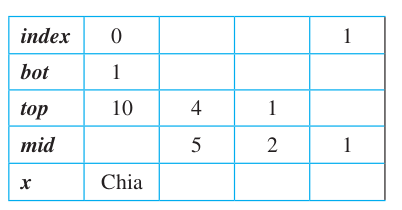
\includegraphics[scale=0.5]{../images/11.5.5.a.png}
\end{figure}
\end{proof}

\subsubsection{(b)}
\(x\) = Max
\begin{proof}
\begin{figure}[ht!]
\centering
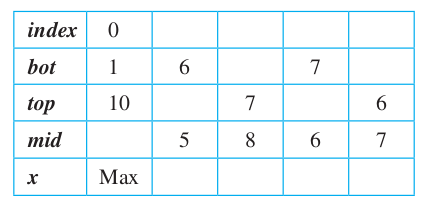
\includegraphics[scale=0.5]{../images/11.5.5.b.png}
\end{figure}
\end{proof}

\subsection{Exercise 6}
(a) \(x\) = Amanda (b) \(x\) = Roy
\begin{proof}
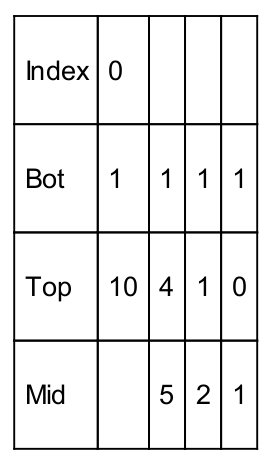
\includegraphics[scale=0.3]{../images/11.5.6.a.png}
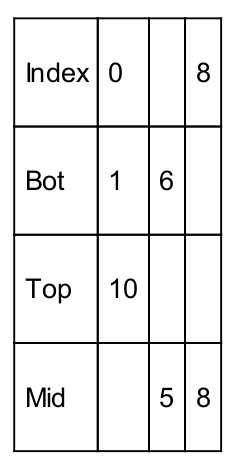
\includegraphics[scale=0.3]{../images/11.5.6.b.png}
\end{proof}

\subsection{Exercise 7}
Suppose \(bot\) and \(top\) are positive integers with \(bot \leq top\). Consider the array 
\(a[bot], a[bot + 1], \ldots, a[top]\).

\subsubsection{(a)}
How many elements are in this array?
\begin{proof}
The array has \(top - bot + 1\) elements.
\end{proof}

\subsubsection{(b)}
Show that if the number of elements in the array is odd, then the quantity \(bot + top\) is even.

\begin{proof}
Suppose \(top\) and \(bot\) are particular but arbitrarily chosen positive integers such that \(top - bot + 1\) is an odd 
number. Then, by definition of odd, there is an integer \(k\) such that \(top - bot + 1 = 2k + 1\). Adding \(2\cdot bot-1\) 
to both sides gives \(bot + top = 2 \cdot bot - 1 + 2k + 1 = 2(bot + k).\) Now \(bot + k\) is an integer. Hence, by 
definition of even, \(bot + top\) is even.
\end{proof}

\subsubsection{(c)}
Show that if the number of elements in the array is even, then the quantity \(bot + top\) is odd.

\begin{proof}
The proof is almost identical to part (b), except with the roles of even and odd swapped.
\end{proof}

{\bf \cy Exercises \(8-11\) refer to the following algorithm segment. For each positive integer \(n\), let \(a_n\) be the 
number of iterations of the while loop.
\begin{center}
{\bf while} \((n > 0)\) \\
\hspace{2cm} \(n \coloneqq n \,\, div \,\, 2\) \\
{\bf end while}
\end{center}
}

\subsection{Exercise 8}
Trace the action of this algorithm segment on \(n\) when the initial value of \(n\) is 27.

\begin{proof}
\(n\): 27, 13, 6, 3, 1, 0
\end{proof}

\subsection{Exercise 9}
Find a recurrence relation for \(a_n\).
\begin{proof}
For each positive integer \(n\), \(n \,\,div\,\, 2 = \floor{n/2}\). Thus when the algorithm segment is run for a particular 
\(n\) and the while loop has iterated one time, the input to the next iteration is \(\floor{n/2}\). It follows that the 
number of iterations of the loop for \(n\) is one more than the number of iterations for \(\floor{n/2}\). That is, 
\(a_n = 1 + a_{\floor{n/2}}\). Also, \(a_1 = 1\).
\end{proof}

\subsection{Exercise 10}
Find an explicit formula for \(a_n\).
\begin{proof}
The recurrence relation and initial condition of \(a_1, a_2, a_3, \ldots\) derived in exercise 9 are the same as those for 
the sequence \(w_1, w_2, w_3, \ldots\) discussed in the worst-case analysis of the binary search algorithm. Thus the general 
formulas for the two sequences are the same. That is, \(a_n = 1 + \floor{\log_2 n}\), for each integer \(n \geq 1\).
\end{proof}

\subsection{Exercise 11}
Find an order for this algorithm segment.

\begin{proof}
In the analysis of the binary search algorithm, it was shown that \(1 + \floor{\log_2 n}\) is \(\Theta(\log_2 n)\). Thus 
the given algorithm segment has order \(\log_2 n\).
\end{proof}

{\bf \cy Exercises \(12-15\) refer to the following algorithm segment. For each positive integer \(n\), let \(b_n\) be the 
number of iterations of the while loop.
\begin{center}
{\bf while} \((n > 0)\) \\
\hspace{2cm} \(n \coloneqq n \,\, div \,\, 3\) \\
{\bf end while}
\end{center}
}

\subsection{Exercise 12}
Trace the action of this algorithm segment on \(n\) when the initial value of \(n\) is 424.

\begin{proof}
\(n\): 424, 141, 47, 15, 5, 1
\end{proof}

\subsection{Exercise 13}
Find a recurrence relation for \(b_n\).

\begin{proof}
For each positive integer \(n\), \(n \,\,div\,\, 3 = \floor{n/3}\). Thus when the algorithm segment is run for a particular 
\(n\) and the while loop has iterated one time, the input to the next iteration is \(\floor{n/3}\). It follows that the 
number of iterations of the loop for \(n\) is one more than the number of iterations for \(\floor{n/3}\). That is, 
\(b_n = 1 + b_{\floor{n/3}}\). Also, \(b_0 = 0, b_1 = 1\).
\end{proof}

\subsection{Exercise 14}
\subsubsection{(a)}
Use iteration to guess an explicit formula for \(b_n\).

\begin{proof}
\(b_1 = 1, b_2 = 1 + b_{\floor{2/3}} = 1 + b_0 = 1, b_3 = 1 + b_{\floor{3/3}} = 1 + b_1 = 1 + 1, \ldots, b_5 = 1+1\),

\(b_6 = 1 + b_{\floor{6/3}} = 1 + b_2 = 1 + 1, \ldots, b_8 = 1 + b_{\floor{8/3}} = 1 + b_2 = 1 + 1\),

\(b_9 = 1 + b_{\floor{9/3}} = 1 + b_3 = 1 + 2 \cdot 1, \ldots, b_{26} = 1 + b_{\floor{26/3}} = 1 + b_8 = 1 + 2 \cdot 1\),

\(b_{27} = 1 + b_{\floor{27/3}} = 1 + b_9 = 1 + 3 \cdot 1\).

Guess: \(b_n = 1 + \floor{\log_3(n)}\).
\end{proof}

\subsubsection{(b)}
Prove that if \(k\) is an integer and \(x\) is a real number with \(3^k \leq x < 3^{k+1}\), then \(\floor{\log_3 x} = k\).

\begin{proof}
Assume \(3^k \leq x < 3^{k+1}\). Since \(\log_3\) is increasing, \(\log_3 3^k \leq \log_3 x < \log_3 3^{k+1}\), or,
\(k \leq \log_3 x < k+1\) by definition of \(\log_3\). Then by definition of floor, \(\floor{\log_3 x} = k\).
\end{proof}

\subsubsection{(c)}
Prove that for every integer \(m \geq1\), \(\floor{\log_3(3m)} = \floor{\log_3(3m + 1)} = \floor{\log_3(3m + 2)}\).

\begin{proof}
1. There exists an integer \(k \geq 0\) such that \(3^k \leq m < 3^{k+1}\).

2. By 1, \(3^{k+1} \leq 3m < 3^{k+2}\). 

3. Notice that the interval \([3^{k+1}, 3^{k+2})\) has size at least 5 or bigger; since \(3^{k+1} \geq 3\) and 
\(3^{k+2} \geq 9\).

4. By 2 and 3, \(3^{k+1} \leq 3m + 1 < 3^{k+2}\) and \(3^{k+1} \leq 3m + 2 < 3^{k+2}\).

5. By 4 and part (b), \(\floor{\log_3(3m)} = \floor{\log_3(3m + 1)} = \floor{\log_3(3m + 2)} = k+1\). 
So they are all equal, {\it [as was to be shown.]}
\end{proof}

\subsubsection{(d)}
Prove the correctness of the formula you found in part (a).

\begin{proof}
Given: \(b_0 = 0, b_1 = 1\), \(b_n = 1 + b_{\floor{n/3}}\), want to prove: \(b_n = 1 + \floor{\log_3(n)}\).

Let \(P(n)\) be the equation: \(b_n = 1 + \floor{\log_3(n)}\).

{\bf Show that \(P(2)\) is true:} \(b_2 = 1 + b_{\floor{2/3}} = 1 + b_0 = 1 + 0 = 1 + \floor{\log_3(2)}\) so \(P(2)\) is 
true.

{\bf Show that for any integer \(k \geq 2\) if \(P(i)\) is true for all \(0 \leq i \leq k\) then \(P(k+1)\) is true:}
Assume \(k \geq 2\) is any integer such that \(b_i = 1 + \floor{\log_3(i)}\) for all \(0 \leq i \leq k\). {\it [This 
is the inductive hypothesis.]} Want to prove: \(b_{k+1} = 1 + \floor{\log_3(k+1)}\).

\(k+1 \geq 3\), so by the quotient-remainder theorem \(k+1 = 3m+j\) for some integers \(1\leq m\geq k\) and \(0\leq j< 3\).

By definition \(b_{k+1} = 1 + b_{\floor{(k+1)/3}} = 1 + b_{\floor{(3m+j)/3}} = 1 + b_{\floor{m + \frac{j}{3}}}\)
\( = 1 + b_m\). This is because \(0 \leq \frac{j}{3} < 1\) so \(m \leq m+\frac{j}{3} < m+1\) and so it follows from the 
definition of floor.

By inductive hypothesis \(b_m = 1 + \floor{\log_3 m}\). So \(b_{k+1} = 1 + 1 + \floor{\log_3 m} = 1 + 1 + \floor{\log_3 
(3m)/3} = 1 + 1 + (\floor{\log_3 (3m) - \log_3 3}) = 1 + 1 + (\floor{\log_3 (3m) - 1}) = 1 + 1 + \floor{\log_3 (3m)} - 1)
= 1 + \floor{\log_3(3m)} = 1 + \floor{\log_3(3m + j)} = 1 + \floor{\log_3 (k+1)}\). (The second to last step follows by part (c) since \(\floor{\log_3 3m} = \floor{\log_3(3m+j)}\)).
\end{proof}

\subsection{Exercise 15}
Find an order for the algorithm segment.

\begin{proof}
Similar to exercise 11, \(b_n\) is \(\Theta(\log_3 n)\) so the order is \(\log_3 n\).
\end{proof}

\subsection{Exercise 16}
Complete the proof of case 2 of the strong induction argument in Example 11.5.5. In other words, show that if \(k\) is an 
odd integer and \(w_i = \floor{\log_2 i} + 1\) for every integer \(i\) with \(1 \leq i \leq k\), then \(w_{k+1} = 
\floor{\log_2 k + 1} + 1\).

\begin{proof}
We are given \(w_1 = 1\) and \(w_{k+1} = 1 + w_{\floor{k/2}}\) for each \(k > 1\).

We want to prove \(w_k = \floor{\log_2 k} + 1\), in the case when \(k\) is odd. Notice \(k\) is at least 3.

So \(k = 2m+1\) for some integer \(m \geq 1\). So \(w_{k+1} = 1 + w_{\floor{k/2}} = 1 + w_{\floor{(2m+1)/2}} = 1 + 
w_{\floor{m + 1/2}} = 1 + w_m\).

By inductive hypothesis \(w_m = 1 + \floor{\log_2 m}\). So \(w_{k+1} = 1 + w_m = 1 + 1 + \floor{\log_2 m} = 1 + 1 + 
\floor{\log_2 (m+1)} = 1 + 1 + \floor{\log_2 (2(m+1)/2)} = 1 + 1 + \floor{\log_2 (2(m+1)) - \log_2 2} = 1 + 1 + \floor{\log_2 
(2(m+1)) - 1} = 1 + 1 + (\floor{\log_2 (2(m+1))} - 1) = 1 + \floor{\log_2 (2m+2)} = 1 + \floor{\log_2 (k+1)}\).

We are using the facts \(\floor{\log_2 m} = \floor{\log_2 (m+1)}\) (by Property 11.4.3 in Exercise 11.4.2) and 
\(\floor{x-1} = \floor{x} - 1\) (Exercise 15 of section 4.6).
\end{proof}

{\bf \cy For \(17-19\), modify the binary search algorithm (Algorithm 11.5.1) to take the upper of the two middle array
elements in case the input array has even length. In other words, in Algorithm 11.5.1 replace \(\dps mid \coloneqq \floor{\frac{bot+top}{2}}\) with \(\dps mid \coloneqq 
\ceil{\frac{bot+top}{2}}\).}

\subsection{Exercise 17}
Trace the modified binary search algorithm for the same input as was used in Example 11.5.1.

\(a[1]\) = Ann, \(a[2]\) = Dawn, \(a[3] =\) Erik, \(a[4] =\) Gail, \(a[5] =\) Juan, \(a[6] =\) Matt, \(a[7] =\) Max, 
\(a[8] =\) Rita, \(a[9] =\) Tsuji, \(a[10] =\) Yuen, \,\,\,
(a) \(x = \) Erik, \,\,\, (b) \(x = \) Sara

\begin{proof}
\arrayrulecolor{cyan}
\begin{tabular}{|c|c|c|c|}
\hline
\(index\)& 0& &3 \\
\hline
\(bot\)  & 1& &  \\
\hline
\(top\)  &10&5&  \\
\hline
\(mid\)  &  &6&3 \\
\hline
\(x\)  &Erik& &  \\
\hline
\end{tabular}
\begin{tabular}{|c|c|c|c|c|c|c|c|c|c|c|c|c|c|}
\hline
\(index\)&0& & &  \\
\hline
\(bot\)  &1&7& &9 \\
\hline
\(top\) &10& &8&  \\
\hline
\(mid\)  & &6&9&8 \\
\hline
\(x\)&Sarah& & &  \\
\hline
\end{tabular}
\arrayrulecolor{black}
\end{proof}

\subsection{Exercise 18}
Suppose an array of length \(k\) is input to the while loop of the modified binary search algorithm. Show that after one 
iteration of the loop, if \(a[mid] \neq x\), the input to the next iteration is an array of length at most \(\floor{k/2}\).

\begin{proof}
1. At the beginning of the loop, \(bot = 1, top = k\). 

2. Therefore \(mid = \floor{(1+k)/2}\). 

For simplicity assume \(k\) is odd, so \(k = 2m+1\) for some \(m\), so \(mid = \floor{(1+2m+1)/2} = m+1\).

3. If \(a[mid] \neq x\) then either \(top = mid - 1 = m\), or \(bot = mid + 1 = m+2\).

4. At the next iteration, either \(bot = 1\) and \(top = m\), or \(bot = m+2\) and \(top = k\).

5. So either \(top - bot = m - 1\) or \(top - bot = k - (m+2) = 2m+1 - m - 2 = m-1\). 

6. So in both cases the size of the input to the next iteration is \(m-1+1 = m = \floor{m + 1/2} = \floor{(2m+1)/2}
= \floor{k/2}\).

7. In later iterations, the interval \([bot, top]\) gets even smaller (because \(bot\) can only increase and \(top\) can 
only decrease), so the size of the input is at most the size after the first iteration, which is \(\floor{k/2}\).

8. The case where \(k\) is even is similar.
\end{proof}

\subsection{Exercise 19}
Let \(w_n\) be the number of iterations of the while loop in a worst-case execution of the modified binary search algorithm 
for an input array of length \(n\). Show that \(w_k = 1 + w_{\floor{k/2}}\) for \(k \geq 2\).

\begin{proof}
By exercise 18, after one iteration of the loop, if \(a[mid] \neq x\), the input to the next iteration is an array of 
length at most \(\floor{k/2}\). So \(w_k\) is one iteration plus the number of iterations of the loop for an input of size
\(\floor{k/2}\), in other words, \(w_k = 1 + \floor{k/2}\).
\end{proof}

{\bf \cy In 20 and 21, draw a diagram like Figure 11.5.4 to show how to merge the given subarrays into a single array in 
ascending order.}

\subsection{Exercise 20}
3, 5, 6, 9, 12 and 2, 4, 7, 9, 11

\begin{proof}
\begin{figure}[ht!]
\centering
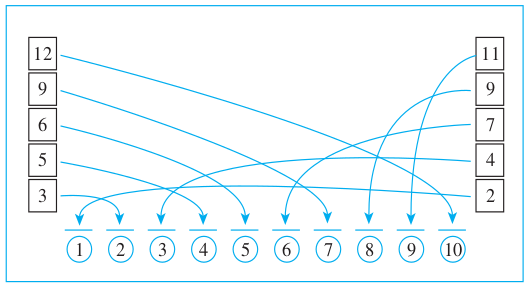
\includegraphics[scale=0.5]{../images/11.5.20.png}
\end{figure}
\end{proof}

\subsection{Exercise 21}
F, K, L, R, U and C, E, L, P, W (alphabetical order)

\begin{proof}
\begin{figure}[ht!]
\centering
\includegraphics[scale=0.3]{../images/11.5.21.png}
\end{figure}
\end{proof}

{\bf \cy In 22 and 23, draw a diagram like Figure 11.5.5 to show how merge sort works for the given input arrays.}

\subsection{Exercise 22}
R, G, B, U, C, F, H, G (alphabetical order)

\begin{proof}
\begin{figure}[ht!]
\centering
\includegraphics[scale=0.5]{../images/11.5.22.png}
\end{figure}
\end{proof}

\subsection{Exercise 23}
5, 2, 3, 9, 7, 4, 3, 2

\begin{proof}
\begin{figure}[ht!]
\centering
\includegraphics[scale=0.4]{../images/11.5.23.png}
\end{figure}
\end{proof}

\subsection{Exercise 24}
Show that given an array \(a[bot], a[bot + 1], \ldots, a[top]\) of length \(k\), if \(mid = \floor{(bot + top)/2}\) then

\subsubsection{(a)}
the subarray \(a[mid + 1], a[mid + 2], \ldots, a[top]\) has length \(\floor{k/2}\).

\begin{proof}
Refer to Figure 11.5.3 and observe that the subarray \(a[mid], a[mid + 1], \ldots, a[top]\) has length \(k - (\frac{k}{2} + 
1) + 1 = \frac{k}{2} = \floor{\frac{k}{2}}\).
\end{proof}

\subsubsection{(b)}
the subarray \(a[bot], a[bot + 1], \ldots, a[mid]\) has length \(\ceil{k/2}\).

\begin{proof}
Refer to Figure 11.5.3 and observe that when \(k\) is even, the subarray \(a[bot], a[bot + 1], \ldots, a[mid]\) has length 
\(\floor{\frac{k}{2}} = \ceil{\frac{k}{2}}\) and when \(k\) is odd, has length \(\floor{\frac{k}{2}}+1=\ceil{\frac{k}{2}}\).
\end{proof}

\subsection{Exercise 25}
The recurrence relation for \(m_1, m_2, m_3, \ldots\), which arises in the calculation of the efficiency of merge sort, is 
\(m_1 = 0, m_k = m_{\floor{k/2}} + m_{\ceil{k/2}} + k - 1\). Show that for every integer \(n \geq 1\) 

\subsubsection{(a)}
\(\frac{1}{2} n \log_2 n \leq m_n\)
\begin{proof}
{\bf Show that \(P(1)\) is true:} \(\frac{1}{2} \cdot 1 \log_2 1 = 0 \leq 0 = m_n\), so \(P(1)\) is true.

{\bf Show that for any integer \(k \geq 1\) if \(P(i)\) is true for all \(1 \leq i \leq k\) then \(P(k+1)\) is true:}
Now if \(k\) is odd and \(k+1\) is even, then \(m_{k+1}\) 

\begin{tabular}{cll}
= & \(m_{\floor{(k+1)/2}} + m_{\ceil{(k+1)/2}} + (k+1) - 1\) & \\
= & \(m_{(k+1)/2} + m_{(k+1)/2} + (k+1) - 1\) & {\cy by Theorem 4.6.2 and Exercise 4.6.19} \\
= & \(2m_{(k+1)/2} + k\) & \\
\(\geq\) & \(\dps 2 \cdot \left[\frac{1}{2} \cdot \frac{k+1}{2} \cdot \log_2\left(\frac{k+1}{2}\right)\right] + k\) & 
{\cy by inductive hypothesis} \\
\(\geq\) & \(\dps \left(\frac{k+1}{2}\right)[\log_2(k+1) - \log_2 2] + k\) & \\
= & \(\frac{1}{2}(k+1)[\log_2(k+1) - 1] + k\) & \\
= & \(\frac{1}{2}(k+1)\log_2(k+1) - \frac{1}{2}(k+1) + \frac{2k}{2}\) & \\
= & \(\frac{1}{2}(k+1)\log_2(k+1) + \frac{1}{2}(k-1)\) & \\
\(\geq\) & \(\frac{1}{2}(k+1)\log_2(k+1)\) & {\cy by algebra} \\
\end{tabular}

The other case where \(k\) is even and \(k+1\) is odd is similar.
\end{proof}

\subsubsection{(b)}
\(m_n \leq 2n \log_2 n\)
\begin{proof}
{\bf Show that \(P(1)\) is true:} \(m_n = 0 = 2(1) \log_2(1)\), so \(P(1)\) is true.

{\bf Show that for any integer \(k \geq 1\) if \(P(i)\) is true for all \(1 \leq i \leq k\) then \(P(k+1)\) is true:}
Now if \(k\) is odd and \(k+1\) is even, then \(m_{k+1}\)

\begin{tabular}{cll}
= & \(m_{\floor{(k+1)/2}} + m_{\ceil{(k+1)/2}} + (k+1) - 1\) & \\
= & \(m_{(k+1)/2} + m_{(k+1)/2} + (k+1) - 1\) & {\cy by Theorem 4.6.2 and Exercise 4.6.19} \\
= & \(2m_{(k+1)/2} + k\) & \\
\(\leq\) & \(2[2\frac{k+1}{2} \log_2\left(\frac{k+1}{2}\right)] + k\) & {\cy by inductive hypothesis} \\
= & \(2(k+1)[\log_2(k+1) - \log_2 2] + k\) &  \\
= & \(2(k+1)[\log_2(k+1) - 1] + k\) &  \\
= & \(2(k+1)\log_2(k+1) - 2(k+1) + k\) & \\
= & \(2(k+1)\log_2(k+1) - k - 2\) &  \\
\(\leq\) & \(2(k+1)\log_2(k+1)\) & {\cy by algebra} \\
\end{tabular}

The other case where \(k\) is even and \(k+1\) is odd is similar.
\end{proof}

\subsection{Exercise 26}
It might seem that \(n - 1\) multiplications are needed to compute \(x^n = \underbrace{x \cdot \cdots \cdot x}_{\cy n - 1 
\text{ multiplications}}\). But observe that, for instance, since \(6 = 4 + 2\), \(x^6 = x^4x^2 = (x^2)^2x^2\). Thus 
\(x^6\) can be computed using three multiplications: one to compute \(x^2\), one to compute \((x^2)^2\), and one to 
multiply \((x^2)^2\) times \(x^2\). Similarly, since \(11 = 8 + 2 + 1\), \(x^{11} = x^8 x^2 x^1 = ((x^2)^2)^2x^2x\) and so 
\(x^{11}\) can be computed using five multiplications: one to compute \(x^2\), one to compute \((x^2)^2\), one to compute 
\(((x^2)^2)^2\), one to multiply \(((x^2)^2)^2\) times \(x^2\), and one to multiply that product by \(x\).

\subsubsection{(a)}
Write an algorithm to take a real number \(x\) and a positive integer \(n\) and compute \(x^n\) by

(i) calling Algorithm 5.1.1 to find the binary representation of \(n\): \((r[k] r[k - 1] \cdots r[0])_2\), where each 
\(r[i]\) is 0 or 1; 

(ii) computing \(x^2, x^{2^2}, x^{2^3}, \ldots, x^{2^k}\) by squaring, then squaring again, and so forth;

(iii) computing \(x^n\) using the fact that 
\[
x^n = x^{r[k]2^k + \cdots + r[1]2^1 + r[0]2^0} = x^{r[k]2^k} \cdot \ldots \cdot x^{r[1]2^2} \cdot x^{r[0]2^0}
\]
\begin{proof}
{\it ???}
\end{proof}

\subsubsection{(b)}
Show that the number of multiplications performed by the algorithm of part (a) is less than or equal to 
\(2\floor{\log_2 n}\).

\begin{proof}
{\it ???}
\end{proof}

\end{document}
